% Options for packages loaded elsewhere
% Options for packages loaded elsewhere
\PassOptionsToPackage{unicode}{hyperref}
\PassOptionsToPackage{hyphens}{url}
\PassOptionsToPackage{dvipsnames,svgnames,x11names}{xcolor}
%
\documentclass[
  brazilian,
  12pt,
  letterpaper,
  DIV=11,
  numbers=noendperiod]{scrartcl}
\usepackage{xcolor}
\usepackage[a4paper,left=3cm,right=2cm,top=3cm,bottom=2cm]{geometry}
\usepackage{amsmath,amssymb}
\setcounter{secnumdepth}{5}
\usepackage{iftex}
\ifPDFTeX
  \usepackage[T1]{fontenc}
  \usepackage[utf8]{inputenc}
  \usepackage{textcomp} % provide euro and other symbols
\else % if luatex or xetex
  \usepackage{unicode-math} % this also loads fontspec
  \defaultfontfeatures{Scale=MatchLowercase}
  \defaultfontfeatures[\rmfamily]{Ligatures=TeX,Scale=1}
\fi
\usepackage{lmodern}
\ifPDFTeX\else
  % xetex/luatex font selection
\fi
% Use upquote if available, for straight quotes in verbatim environments
\IfFileExists{upquote.sty}{\usepackage{upquote}}{}
\IfFileExists{microtype.sty}{% use microtype if available
  \usepackage[]{microtype}
  \UseMicrotypeSet[protrusion]{basicmath} % disable protrusion for tt fonts
}{}
\usepackage{setspace}
\makeatletter
\@ifundefined{KOMAClassName}{% if non-KOMA class
  \IfFileExists{parskip.sty}{%
    \usepackage{parskip}
  }{% else
    \setlength{\parindent}{0pt}
    \setlength{\parskip}{6pt plus 2pt minus 1pt}}
}{% if KOMA class
  \KOMAoptions{parskip=half}}
\makeatother
% Make \paragraph and \subparagraph free-standing
\makeatletter
\ifx\paragraph\undefined\else
  \let\oldparagraph\paragraph
  \renewcommand{\paragraph}{
    \@ifstar
      \xxxParagraphStar
      \xxxParagraphNoStar
  }
  \newcommand{\xxxParagraphStar}[1]{\oldparagraph*{#1}\mbox{}}
  \newcommand{\xxxParagraphNoStar}[1]{\oldparagraph{#1}\mbox{}}
\fi
\ifx\subparagraph\undefined\else
  \let\oldsubparagraph\subparagraph
  \renewcommand{\subparagraph}{
    \@ifstar
      \xxxSubParagraphStar
      \xxxSubParagraphNoStar
  }
  \newcommand{\xxxSubParagraphStar}[1]{\oldsubparagraph*{#1}\mbox{}}
  \newcommand{\xxxSubParagraphNoStar}[1]{\oldsubparagraph{#1}\mbox{}}
\fi
\makeatother


\usepackage{longtable,booktabs,array}
\newcounter{none} % for unnumbered tables
\usepackage{calc} % for calculating minipage widths
% Correct order of tables after \paragraph or \subparagraph
\usepackage{etoolbox}
\makeatletter
\patchcmd\longtable{\par}{\if@noskipsec\mbox{}\fi\par}{}{}
\makeatother
% Allow footnotes in longtable head/foot
\IfFileExists{footnotehyper.sty}{\usepackage{footnotehyper}}{\usepackage{footnote}}
\makesavenoteenv{longtable}
\usepackage{graphicx}
\makeatletter
\newsavebox\pandoc@box
\newcommand*\pandocbounded[1]{% scales image to fit in text height/width
  \sbox\pandoc@box{#1}%
  \Gscale@div\@tempa{\textheight}{\dimexpr\ht\pandoc@box+\dp\pandoc@box\relax}%
  \Gscale@div\@tempb{\linewidth}{\wd\pandoc@box}%
  \ifdim\@tempb\p@<\@tempa\p@\let\@tempa\@tempb\fi% select the smaller of both
  \ifdim\@tempa\p@<\p@\scalebox{\@tempa}{\usebox\pandoc@box}%
  \else\usebox{\pandoc@box}%
  \fi%
}
% Set default figure placement to htbp
\def\fps@figure{htbp}
\makeatother


% definitions for citeproc citations
\NewDocumentCommand\citeproctext{}{}
\NewDocumentCommand\citeproc{mm}{%
  \begingroup\def\citeproctext{#2}\cite{#1}\endgroup}
\makeatletter
 % allow citations to break across lines
 \let\@cite@ofmt\@firstofone
 % avoid brackets around text for \cite:
 \def\@biblabel#1{}
 \def\@cite#1#2{{#1\if@tempswa , #2\fi}}
\makeatother
\newlength{\cslhangindent}
\setlength{\cslhangindent}{1.5em}
\newlength{\csllabelwidth}
\setlength{\csllabelwidth}{3em}
\newenvironment{CSLReferences}[2] % #1 hanging-indent, #2 entry-spacing
 {\begin{list}{}{%
  \setlength{\itemindent}{0pt}
  \setlength{\leftmargin}{0pt}
  \setlength{\parsep}{0pt}
  % turn on hanging indent if param 1 is 1
  \ifodd #1
   \setlength{\leftmargin}{\cslhangindent}
   \setlength{\itemindent}{-1\cslhangindent}
  \fi
  % set entry spacing
  \setlength{\itemsep}{#2\baselineskip}}}
 {\end{list}}
\usepackage{calc}
\newcommand{\CSLBlock}[1]{\hfill\break\parbox[t]{\linewidth}{\strut\ignorespaces#1\strut}}
\newcommand{\CSLLeftMargin}[1]{\parbox[t]{\csllabelwidth}{\strut#1\strut}}
\newcommand{\CSLRightInline}[1]{\parbox[t]{\linewidth - \csllabelwidth}{\strut#1\strut}}
\newcommand{\CSLIndent}[1]{\hspace{\cslhangindent}#1}

\ifLuaTeX
\usepackage[bidi=basic,shorthands=off]{babel}
\else
\usepackage[bidi=default,shorthands=off]{babel}
\fi
\ifLuaTeX
  \usepackage{selnolig} % disable illegal ligatures
\fi


\setlength{\emergencystretch}{3em} % prevent overfull lines

\providecommand{\tightlist}{%
  \setlength{\itemsep}{0pt}\setlength{\parskip}{0pt}}



 


% Impede o sumário de colar na capa
\usepackage{tocloft}
\setcounter{tocdepth}{3}
\usepackage{placeins}
\usepackage{pdflscape}
\usepackage{booktabs}
\usepackage{longtable}
\usepackage{array}
\usepackage{multirow}
\usepackage{wrapfig}
\usepackage{float}
\usepackage{colortbl}
\usepackage{pdflscape}
\usepackage{tabu}
\usepackage{threeparttable}
\usepackage{threeparttablex}
\usepackage[normalem]{ulem}
\usepackage{makecell}
\usepackage{xcolor}
\usepackage{caption}
\usepackage{anyfontsize}
\KOMAoption{captions}{tableheading}
\usepackage{xcolor}
\newcommand{\red}[1]{\textcolor{red}{#1}}
\newcommand{\blue}[1]{\textcolor{blue}{#1}}
\makeatletter
\@ifpackageloaded{caption}{}{\usepackage{caption}}
\AtBeginDocument{%
\ifdefined\contentsname
  \renewcommand*\contentsname{Índice}
\else
  \newcommand\contentsname{Índice}
\fi
\ifdefined\listfigurename
  \renewcommand*\listfigurename{Lista de Figuras}
\else
  \newcommand\listfigurename{Lista de Figuras}
\fi
\ifdefined\listtablename
  \renewcommand*\listtablename{Lista de Tabelas}
\else
  \newcommand\listtablename{Lista de Tabelas}
\fi
\ifdefined\figurename
  \renewcommand*\figurename{Figura}
\else
  \newcommand\figurename{Figura}
\fi
\ifdefined\tablename
  \renewcommand*\tablename{Tabela}
\else
  \newcommand\tablename{Tabela}
\fi
}
\@ifpackageloaded{float}{}{\usepackage{float}}
\floatstyle{ruled}
\@ifundefined{c@chapter}{\newfloat{codelisting}{h}{lop}}{\newfloat{codelisting}{h}{lop}[chapter]}
\floatname{codelisting}{Listagem}
\newcommand*\listoflistings{\listof{codelisting}{Lista de Listagens}}
\makeatother
\makeatletter
\makeatother
\makeatletter
\@ifpackageloaded{caption}{}{\usepackage{caption}}
\@ifpackageloaded{subcaption}{}{\usepackage{subcaption}}
\makeatother
\usepackage{bookmark}
\IfFileExists{xurl.sty}{\usepackage{xurl}}{} % add URL line breaks if available
\urlstyle{same}
\hypersetup{
  pdflang={pt-BR},
  colorlinks=true,
  linkcolor={blue},
  filecolor={Maroon},
  citecolor={Blue},
  urlcolor={Blue},
  pdfcreator={LaTeX via pandoc}}


\author{}
\date{}
\begin{document}


\setstretch{1.5}
\begin{titlepage}
\centering

% --- IMAGEM NO TOPO ---

\includegraphics[width=0.3\textwidth]{figuras/logo_ufmg.jpg}

{\large UNIVERSIDADE FEDERAL DE MINAS GERAIS \par}
{\large Instituto de Ciências Exatas \par}
{\large Departamento de Ciência da Computação e Estatística \par}
{\large Pós-Graduação Lato Sensu em Ciência de Dados \par}

\vspace{2cm}

{\bfseries\Large Uma Análise Comparativa entre Inferência Frequentista e Bayesiana em Modelos de Regressão Binária Aplicada a Risco de Crédito \par}

\vspace{2cm}

{\large Ana Beatriz Coelho Rodrigues \par}

\vfill

{\large Belo Horizonte \par}


{\large Dez/2026 \par}

\end{titlepage}

\newpage
\begin{center}

Ana Beatriz Coelho Rodrigues

\vspace{1cm}

{\bfseries\Large Uma Análise Comparativa entre Inferência Frequentista e Bayesiana em Modelos de Regressão Binária Aplicada a Risco de Crédito}


\vspace{2cm}

\begin{flushright}
Monografia apresentada ao Curso de Especialização em Ciência de Dados com Ênfase em Estatística da Universidade Federal de Minas Gerais como requisito parcial para obtenção do grau de Especialista em Ciência de Dados.


\vspace{1cm}

Orientador(a): Prof.(a) Dr.(a) Fábio N. Demarqui~
\end{flushright}

\vfill

Belo Horizonte  

Dez/2026
\end{center}
\newpage

\newpage
\begin{center}
{\bfseries\Large RESUMO}
\end{center}

\vspace{1cm}

Este trabalho compara as abordagens de inferência frequentista e bayesiana na modelagem da probabilidade de inadimplência em cartões de crédito, utilizando o conjunto de dados \textit{Default of Credit Card Clients}, composto por 30.000 registros de clientes taiwaneses. Foram ajustados modelos de regressão logística sob as duas perspectivas: quatro especificações frequentistas (modelo completo, sem multicolinearidade, com regularização L1 e L2) e dois modelos bayesianos com distribuições a priori Normal e Laplace, igualadas em variância para controlar a comparação.

Do ponto de vista preditivo, todas as especificações apresentaram desempenho semelhante, com ROC AUC entre 0,714 e 0,717, sugerindo que, em amostras de grande dimensão, a escolha entre as abordagens não determina diferenças relevantes na capacidade discriminativa. A variável de maior impacto foi o histórico de atraso de pagamento (\texttt{atraso\_pagto\_0}), com razão de chances superior a 1,82 nas estimativas frequentistas e 1,93 nas bayesianas padronizadas. A remoção de preditores altamente correlacionados reduziu substancialmente a multicolinearidade (VIF de 41,12 para 1,84) sem comprometer o desempenho preditivo.

A comparação entre as prioris Normal e Laplace revelou estimativas posteriores praticamente equivalentes, resultado consistente com o teorema de Bernstein-von Mises: com $n = 30.000$, a verossimilhança domina a distribuição posterior, atenuando a influência da priori. A principal diferença entre as abordagens reside na dimensão inferencial: os intervalos de credibilidade bayesianos permitem interpretação probabilística direta sobre os parâmetros, em contraste com os intervalos de confiança frequentistas.

\vspace{1cm}

\noindent\textbf{Palavras-chave:} regressão logística; inferência frequentista; inferência bayesiana; risco de crédito; distribuições a priori.
\newpage

\newpage
\begin{center}
{\bfseries\Large ABSTRACT}
\end{center}

\vspace{1cm}

This study compares frequentist and Bayesian inference approaches in the modeling of credit card default probability, using the Default of Credit Card Clients dataset, comprising 30,000 records from Taiwanese credit card clients. Logistic regression models were fitted under both perspectives: four frequentist specifications (full model, without multicollinearity, with L1 and L2 regularization) and two Bayesian models with Normal and Laplace prior distributions, matched in variance to enable a controlled comparison.

From a predictive standpoint, all specifications yielded similar performance, with ROC AUC ranging from 0.714 to 0.717, suggesting that, in large samples, the choice between approaches does not lead to relevant differences in discriminative capacity. The most influential predictor was payment delay history (\texttt{atraso\_pagto\_0}), with odds ratios above 1.82 in frequentist estimates and 1.93 in standardized Bayesian estimates. Removal of highly correlated predictors substantially reduced multicollinearity (VIF from 41.12 to 1.84) without compromising predictive performance.

The comparison between Normal and Laplace priors revealed nearly equivalent posterior estimates, consistent with the Bernstein-von Mises theorem: with n = 30,000, the likelihood dominates the posterior distribution, attenuating prior influence. The main distinction between approaches lies in the inferential dimension: Bayesian credibility intervals allow direct probabilistic statements about parameters, in contrast to the repeated-sampling interpretation of frequentist confidence intervals.


\vspace{1cm}

\noindent\textbf{Keywords:} logistic regression; frequentist inference; Bayesian inference; credit risk; prior distributions.
\newpage

\tableofcontents
\newpage

\section{Introdução}\label{introduuxe7uxe3o}

A atividade de concessão de crédito envolve decisões tomadas sob
incerteza, nas quais existe sempre a possibilidade de que o tomador não
cumpra integralmente suas obrigações financeiras. Esse descumprimento
pode manifestar-se na forma de atrasos, pagamentos parciais ou
inadimplência total, e está frequentemente associado a mudanças
inesperadas nas condições econômicas ou financeiras do indivíduo, como
perda de renda, instabilidade profissional ou choques temporários de
liquidez. Mesmo tomadores com histórico financeiro consistente não estão
imunes a esse tipo de risco ao longo do tempo.

A avaliação do risco de crédito é, portanto, um componente central da
gestão financeira das instituições que operam no mercado de empréstimos
e concessão de crédito. Do ponto de vista operacional, essa avaliação
subsidia decisões relacionadas à aprovação ou rejeição de propostas de
crédito, bem como à definição de condições contratuais compatíveis com o
nível de risco assumido. Em uma perspectiva mais ampla, a estimativa da
probabilidade de inadimplência em nível agregado permite antecipar
perdas potenciais e orientar estratégias de alocação de capital,
fundamentais para a estabilidade financeira das instituições. Uma
concentração excessiva de inadimplência pode comprometer a solvência de
intermediários financeiros, tornando indispensável a adoção de
mecanismos preventivos de controle e monitoramento do risco.

Nesse cenário, modelos estatísticos têm sido amplamente empregados como
ferramentas para quantificar o risco de crédito a partir de informações
observáveis sobre os tomadores. Ao relacionar características
socioeconômicas, financeiras e comportamentais com a ocorrência de
inadimplência, esses modelos permitem estimar probabilidades individuais
de default e identificar padrões relevantes para a gestão do portfólio
de crédito. Além de contribuir para a redução de perdas esperadas, tais
modelos oferecem suporte à tomada de decisão baseada em evidências,
reforçando a eficiência e a consistência das políticas de concessão de
crédito.

\subsection{Probabilidade de Inadimplência
(PD)}\label{probabilidade-de-inadimpluxeancia-pd}

No contexto da concessão de crédito, a mensuração do risco associado a
cada operação exige mais do que a simples distinção entre bons e maus
pagadores. É necessário quantificar, de forma probabilística, a chance
de que um tomador venha a entrar em inadimplência dentro de um horizonte
de tempo específico. Essa medida é conhecida como
\texttt{Probability\ of\ Default} (PD) e constitui um dos pilares
centrais da gestão moderna de risco de crédito.

A PD representa a probabilidade de que um contrato de crédito apresente
um evento de default definido previamente, como atraso superior a um
determinado número de dias ou a incapacidade total de honrar os
pagamentos. Ao contrário de abordagens puramente classificatórias, a
modelagem da PD fornece uma escala contínua de risco, permitindo ordenar
tomadores de acordo com sua propensão ao default e estabelecer políticas
diferenciadas de concessão, precificação e monitoramento. Essa
característica torna a PD particularmente relevante tanto para decisões
individuais, como a aprovação de um empréstimo, quanto para avaliações
agregadas do risco da carteira.

\subsection{Regressão Logística na Modelagem do Risco de
Crédito}\label{regressuxe3o-loguxedstica-na-modelagem-do-risco-de-cruxe9dito}

A estimação da probabilidade de inadimplência pode ser conduzida por
meio de modelos estatísticos que relacionam uma variável resposta
binária a um conjunto de variáveis explicativas. Entre as alternativas
disponíveis, a regressão logística destaca-se por sua adequação a esse
tipo de problema, uma vez que permite modelar diretamente a
probabilidade de ocorrência de um evento, restringindo as estimativas ao
intervalo entre zero e um.

No contexto do risco de crédito, essa abordagem possibilita investigar
como características demográficas, condições financeiras e histórico de
pagamentos estão associados à ocorrência de inadimplência. Além da
estimativa das probabilidades individuais, a regressão logística oferece
parâmetros interpretáveis, cuja análise permite avaliar a direção e a
intensidade das associações entre os preditores e o evento de interesse.
Dessa forma, o modelo reúne características relevantes tanto para a
investigação inferencial quanto para a construção de ferramentas de
classificação e previsão de risco.

\subsection{Abordagens Inferenciais na Regressão
Logística}\label{abordagens-inferenciais-na-regressuxe3o-loguxedstica}

A estimação dos parâmetros de um modelo de regressão logística pode ser
realizada sob diferentes perspectivas inferenciais, entre as quais se
destacam as abordagens frequentista e bayesiana. Embora ambas utilizem a
informação contida nos dados para produzir estimativas e avaliar a
incerteza associada aos parâmetros, elas se fundamentam em
interpretações distintas da probabilidade e do processo de inferência.

Na perspectiva frequentista, os parâmetros são tratados como quantidades
fixas estimadas por máxima verossimilhança, com a incerteza expressa por
intervalos de confiança; na bayesiana, são variáveis aleatórias, e a
inferência combina a verossimilhança com distribuições a priori para
produzir distribuições a posteriori. Os fundamentos e as diferenças
conceituais entre essas perspectivas são discutidos em detalhe no
Referencial Teórico.

A comparação entre essas perspectivas é particularmente relevante em
problemas de risco de crédito, nos quais a qualidade das estimativas e a
quantificação da incerteza podem influenciar a interpretação dos fatores
associados à inadimplência. Além disso, a abordagem bayesiana permite
investigar o efeito de diferentes especificações de distribuições a
priori sobre os parâmetros estimados, introduzindo uma dimensão
adicional à análise comparativa.

\subsection{Delimitação e Objetivos do
Estudo}\label{delimitauxe7uxe3o-e-objetivos-do-estudo}

Diante dessas considerações, este trabalho investiga a aplicação de
modelos de regressão logística à previsão de inadimplência em cartões de
crédito, sob as perspectivas frequentista e bayesiana. Para isso,
utiliza-se a base de dados \emph{Default of Credit Card Clients}, que
reúne informações de 30.000 clientes e contempla características
demográficas, limite de crédito, valores de faturas e histórico de
pagamentos. A variável resposta, denominada \texttt{PD30}, identifica a
ocorrência de inadimplência no mês subsequente, caracterizando um
problema de classificação binária.

A questão que orienta a pesquisa é: \textbf{em que medida as abordagens
frequentista e bayesiana produzem resultados distintos na estimação,
interpretação e previsão da inadimplência em cartões de crédito, e como
diferentes distribuições a priori influenciam os resultados da
inferência bayesiana?}

Assim, o objetivo geral deste trabalho é comparar as abordagens
frequentista e bayesiana na modelagem da inadimplência em cartões de
crédito por meio da regressão logística, considerando aspectos
inferenciais e preditivos.

\section{Referencial Teórico}\label{referencial-teuxf3rico}

\subsection{Fundamentos de Probabilidade e Inferência
Estatística}\label{fundamentos-de-probabilidade-e-inferuxeancia-estatuxedstica}

\subsubsection{Variáveis Aleatórias e Distribuições de
Probabilidade}\label{variuxe1veis-aleatuxf3rias-e-distribuiuxe7uxf5es-de-probabilidade}

A formalização da incerteza em experimentos aleatórios ocorre por meio
de variáveis aleatórias, que representam os resultados de um espaço
amostral em uma escala numérica. Essa estrutura fundamenta o tratamento
quantitativo de dados e a construção de modelos de probabilidade,
servindo de base para a inferência estatística e machine learning.

As variáveis aleatórias são classificadas em discretas ou contínuas, a
depender da natureza de seu suporte. As discretas assumem valores em
conjuntos finitos ou enumeráveis, como a decisão de aprovação de crédito
ou o número de ocorrências de inadimplência. Já as contínuas podem
assumir qualquer valor em intervalos reais, como a renda dos
proponentes. A incerteza inerente a essas variáveis é formalizada por
distribuições de probabilidade: no domínio discreto, pela função de
massa de probabilidade e, no contínuo, pela função densidade de
probabilidade. Tais funções não apenas sintetizam a natureza
probabilística das variáveis, mas viabilizam o cálculo de medidas
fundamentais, como esperança, variância e probabilidades condicionais,
elementos centrais para a modelagem de risco. A escolha apropriada de
distribuições de probabilidade é fundamental para capturar a
variabilidade dos dados observados e para a construção de modelos
inferenciais capazes de quantificar a incerteza associada às previsões.

\subsubsection{Inferência
Estatística}\label{inferuxeancia-estatuxedstica}

A inferência estatística reúne os métodos que permitem extrair
conclusões sobre uma população ampla a partir de uma amostra reduzida.
Na prática, quando não é viável analisar cada indivíduo ou produto de um
grupo inteiro, utilizamos os dados amostrais para realizar estimativas e
previsões, fundamentadas em modelos que conectam o que observamos aos
parâmetros que desejamos descobrir.

O elemento central desse processo é a aceitação da incerteza. Como os
dados estão sujeitos a variações e erros de medição, a inferência
utiliza estruturas probabilísticas para descrever o comportamento da
população (o conjunto total de elementos) com base na amostra, que é o
subconjunto efetivamente analisado. Como a população é quase sempre
muito maior que a amostra, as conclusões obtidas não são certezas
absolutas, mas sim afirmações probabilísticas. O processo consiste em
utilizar uma amostra aleatória para testar o modelo estatístico que
representa a população, acompanhando cada conclusão de uma medida que
quantifica o seu grau de confiabilidade. Esse caminho envolve escolher
um modelo adequado para o fenômeno e deduzir informações sobre seus
parâmetros desconhecidos.

\subsubsection{Interpretações da
probabilidade}\label{interpretauxe7uxf5es-da-probabilidade}

A noção de probabilidade ocupa um papel central na inferência
estatística, sendo a base para quantificar e interpretar a incerteza.
Atualmente, essa análise é conduzida por dois grandes paradigmas, o
frequentista e o bayesiano, que se distinguem essencialmente na
interpretação do conceito de probabilidade e no tratamento da incerteza
dos parâmetros.

Na abordagem frequentista, tradicionalmente associada à estatística
clássica, a probabilidade é entendida a partir da repetição de um
experimento sob as mesmas condições. Dentro dessa visão, a probabilidade
é vista como uma característica objetiva do processo que gera os dados,
e não como algo que depende do observador. Os dados coletados são
tratados como realizações aleatórias, enquanto os parâmetros do modelo
estatístico que descreve a população são considerados valores fixos,
ainda que desconhecidos. Assim, a incorporação de novas observações não
altera diretamente o conceito de probabilidade, mas contribui para
estimativas mais precisas desses parâmetros por meio de métodos
inferenciais.

Já na abordagem bayesiana, a probabilidade assume um papel mais amplo,
sendo interpretada como um grau de crença ou plausibilidade em uma
afirmação, condicionado às informações disponíveis. Nesse contexto,
probabilidades podem ser atribuídas não apenas a eventos observáveis,
mas também a hipóteses e parâmetros do modelo. Os parâmetros
desconhecidos são tratados como variáveis aleatórias, cuja incerteza é
descrita por distribuições de probabilidade. O conhecimento prévio pode
ser incorporado por meio de distribuições a priori e, à medida que novos
dados são observados, esse conhecimento é atualizado de forma
sistemática pelo teorema de Bayes, resultando em uma distribuição a
posteriori que combina informação prévia e evidência empírica.

\subsubsection{Teorema de Bayes}\label{sec-teorema-bayes}

O Teorema de Bayes constitui o fundamento da inferência bayesiana,
estabelecendo uma regra para atualizar o conhecimento sobre um parâmetro
desconhecido à medida que novas evidências são observadas.
Diferentemente da abordagem frequentista, na qual os parâmetros são
considerados fixos, a inferência bayesiana representa a incerteza sobre
esses parâmetros por meio de distribuições de probabilidade.

Matematicamente, o Teorema de Bayes é expresso por:

\begin{equation}
p(\theta \mid y) =
\frac{p(y \mid \theta)\,p(\theta)}
{p(y)},
\label{eq:bayes}
\end{equation}

em que:

\begin{itemize}
\item
  \(p(\theta \mid y)\) é a \textbf{distribuição a posteriori},
  representando o conhecimento atualizado sobre o parâmetro \(\theta\)
  após a observação dos dados \(y\);
\item
  \(p(y \mid \theta)\) é a \textbf{função de verossimilhança}, que
  quantifica a probabilidade de observar os dados para um determinado
  valor do parâmetro;
\item
  \(p(\theta)\) é a \textbf{distribuição a priori}, responsável por
  representar o conhecimento ou as crenças existentes sobre o parâmetro
  antes da observação dos dados;
\item
  \(p(y)\) é a \textbf{distribuição marginal dos dados}, também
  denominada evidência, dada por
\end{itemize}

\begin{equation}
p(y)=\int p(y\mid\theta)p(\theta)\,d\theta,
\label{eq:evidence}
\end{equation}

a qual garante que a distribuição a posteriori seja devidamente
normalizada, isto é, que sua integral seja igual a um.

Em termos conceituais, o Teorema de Bayes estabelece que a distribuição
a posteriori é proporcional ao produto entre a verossimilhança e a
distribuição a priori, isto é,

\begin{equation}
p(\theta \mid y) \propto p(y \mid \theta)\,p(\theta),
\label{eq:posterior_prop}
\end{equation}

visto que o termo \(p(y)\) não depende do parâmetro \(\theta\). Na
prática, essa forma proporcional é frequentemente utilizada em métodos
computacionais de inferência, como os algoritmos de Monte Carlo via
Cadeias de Markov (MCMC), nos quais não é necessário calcular
explicitamente a constante de normalização.

\subsection{Regressão Logística
Frequentista}\label{regressuxe3o-loguxedstica-frequentista}

Seja \(Y\) a variável resposta, assumindo valor \(Y = 1\) quando ocorre
inadimplência e \(Y = 0\) caso contrário. O objetivo do modelo consiste
em estimar a probabilidade condicional de ocorrência desse evento,
representada por \(P(Y = 1 \mid \theta)\), em que \(\theta\) denota a
probabilidade de inadimplência associada a um determinado tomador.
Assumindo que \(Y\) segue uma distribuição de Bernoulli, tem-se que
\(P(Y = 1 \mid \theta) = \theta\), enquanto a probabilidade de não
ocorrência do evento é dada por \(P(Y = 0 \mid \theta) = 1 - \theta\).
Dessa forma, o parâmetro \(\theta\) corresponde diretamente à
Probabilidade de Inadimplência (PD), principal quantidade de interesse
na modelagem de risco de crédito.

Diversos modelos podem ser utilizados para estimar essa probabilidade em
função das características observadas dos tomadores. Neste trabalho,
será empregada a regressão logística, por se tratar de um dos modelos
mais difundidos para problemas de resposta binária, oferecendo
estimativas probabilísticas de fácil interpretação e ampla aplicação em
modelos de credit scoring.

\subsubsection{Formulação do modelo}\label{formulauxe7uxe3o-do-modelo}

O objetivo da regressão logística consiste, portanto, em modelar a
probabilidade de ocorrência do evento de interesse como uma função das
variáveis explicativas observadas. Em vez de considerar uma única
probabilidade para toda a população, admite-se que cada observação \(i\)
possui sua própria probabilidade de inadimplência, denotada por
\(\theta_i\). Dessa forma,

\begin{equation}
Y_i \mid \theta_i \sim \mathrm{Bernoulli}(\theta_i),
\label{eq:bernoulli_model}
\end{equation}

onde

\begin{equation}
P(Y_i = 1 \mid \theta_i) = \theta_i
\qquad \text{e} \qquad
P(Y_i = 0 \mid \theta_i) = 1 - \theta_i.
\label{eq:bernoulli_prob}
\end{equation}

O objetivo da regressão logística é modelar a probabilidade \(\theta_i\)
em função das variáveis explicativas. Entretanto, como probabilidades
estão restritas ao intervalo \((0,1)\), não é adequado modelá-las
diretamente por meio de uma combinação linear dos preditores. Para
contornar essa limitação, utiliza-se uma função de ligação que
transforma a probabilidade em uma quantidade definida em toda a reta
real. Na regressão logística, essa transformação é realizada pela função
logit, definida por

\begin{equation}
\theta = \log\left(\frac{\theta}{1 - \theta}\right).
\label{eq:logit}
\end{equation}

A equação acima descreve a transformação da probabilidade para a escala
dos logaritmos das chances (log-odds). Como o objetivo do modelo é
estimar probabilidades, após modelar essa quantidade como uma função
linear das variáveis explicativas aplica-se a transformação inversa da
função logit, denominada função logística (ou função sigmoide). Enquanto
a função logit transforma probabilidades em valores pertencentes à reta
real, a função logística realiza o processo inverso, convertendo o
preditor linear em uma probabilidade restrita ao intervalo (0,1). Assim,
definindo o preditor linear como
\begin{equation}\protect\phantomsection\label{eq-preditor-linear}{
\eta_i=\beta_0+\beta_1x_{i1}+\cdots+\beta_px_{ip}
}\end{equation}

em que \(\beta_0\) representa o intercepto do modelo e \(\beta_j\)
(\(j=1,\ldots,p\)) corresponde ao coeficiente associado à variável
explicativa \(x_{ij}\). Dessa forma, o preditor linear resume, em um
único valor, o efeito conjunto de todas as covariáveis sobre a resposta.
Então a probabilidade de ocorrência do evento é dada por

\begin{equation}\protect\phantomsection\label{eq-funcao-logistica}{
\theta_i=\frac{1}{1+\exp(-\eta_i)}.
}\end{equation}

A Figura~\ref{fig-function-logitica} ilustra o comportamento da função
logística para um modelo com uma única variável preditora, considerando
\(\beta_0 = 0\) e \(\beta_1 = 1\). Observa-se que, à medida que o
preditor linear aumenta, a probabilidade do evento cresce,
aproximando-se de zero para valores muito negativos e de um para valores
muito positivos. O ponto de inflexão da curva ocorre quando
\(\eta_i = 0\), situação em que a probabilidade do evento é igual a 0,5.

\begin{figure}

\centering{

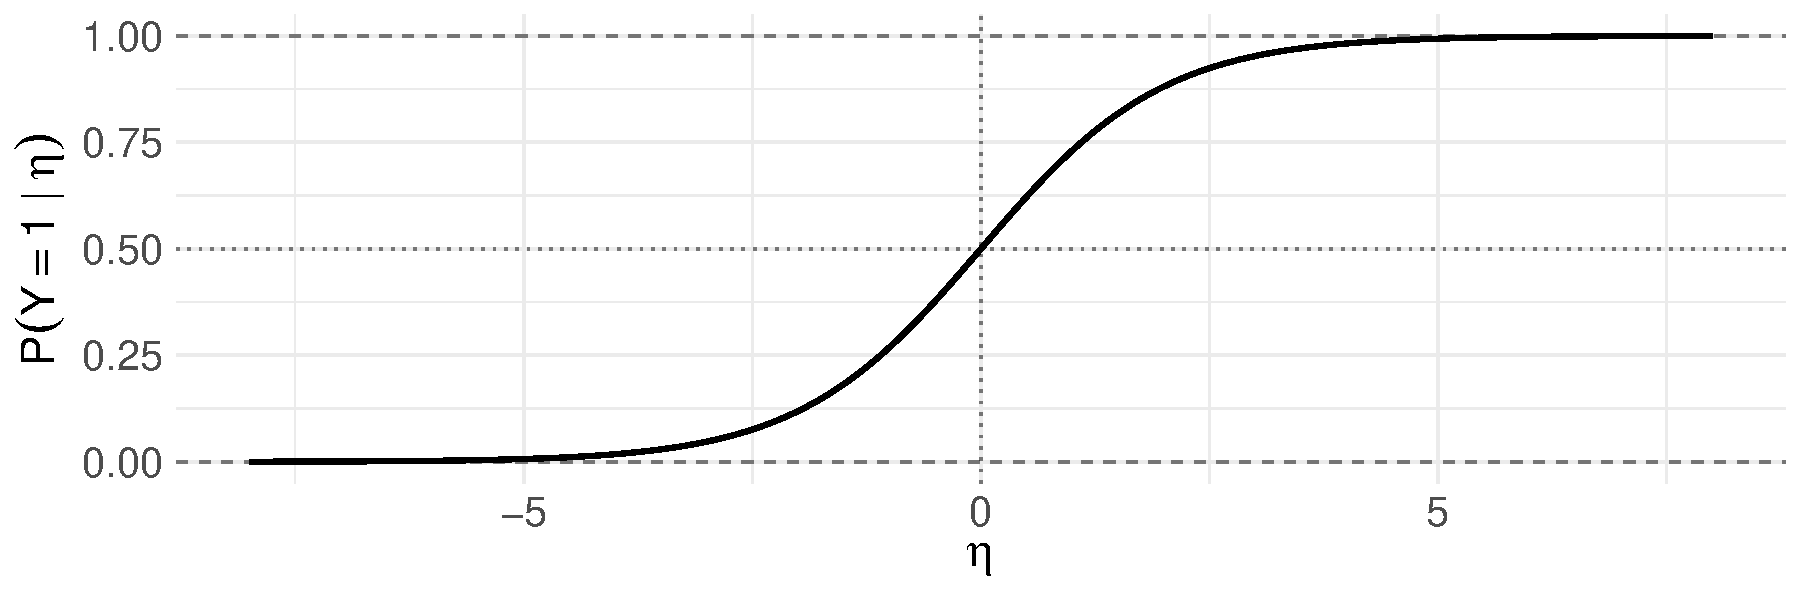
\includegraphics[width=1\linewidth,height=\textheight,keepaspectratio]{monografia_v2_files/figure-pdf/fig-function-logitica-1.pdf}

}

\caption{\label{fig-function-logitica}Função logística para um modelo
com uma única variável preditora (\(\beta_0 = 0\) e \(\beta_1 = 1\)).}

\end{figure}%

\subsubsection{Interpretação dos coeficientes}\label{sec-interpre-coefs}

Como exemplo, considere o seguinte modelo de crédito: \[
\eta = -3 + 0.04 \cdot \text{Score} - 0.8 \cdot \text{Atraso} + 0.2 \cdot \text{Renda}.
\]

Para um determinado solicitante, a substituição dos valores observados
das variáveis explicativas resulta em um valor para \(\eta\). Supondo
que, para esse indivíduo, obtenha-se \(\eta = 1.5\), a função logística
fornece a probabilidade estimada de ocorrência do evento como

\[
\theta = \frac{1}{1+\exp(-1.5)} \approx 0.82.
\]

Esse exemplo evidencia o funcionamento da regressão logística:
inicialmente, as variáveis explicativas são combinadas linearmente para
produzir o preditor \(\eta\); em seguida, a função logística transforma
esse valor em uma probabilidade pertencente ao intervalo \((0,1)\).

Uma das principais vantagens da regressão logística é a possibilidade de
interpretar o efeito das variáveis explicativas sobre o risco do evento
de interesse. Considerando o preditor linear apresentado na
Equação~\ref{eq-preditor-linear}, cada coeficiente \(\beta_j\)
representa a variação esperada no logaritmo das chances
(\emph{log-odds}) associada ao aumento de uma unidade da variável
\(x_j\), mantendo as demais variáveis constantes.

No modelo apresentado anteriormente, o coeficiente associado à variável
\textbf{Score} é igual a \(0.04\). Isso significa que, para cada aumento
de uma unidade no Score, o preditor linear \(\eta\) aumenta em \(0.04\),
desde que as demais variáveis permaneçam constantes. De forma análoga,
cada atraso adicional reduz o preditor linear em \(0.8\) unidades.

Como a função logística é crescente, coeficientes positivos aumentam a
probabilidade estimada do evento, enquanto coeficientes negativos a
reduzem. Entretanto, esse efeito não corresponde a um aumento constante
da probabilidade. Um mesmo incremento em \(\eta\) pode produzir
variações distintas em \(\theta\), dependendo da região da curva
logística em que a observação se encontra.

Para ilustrar esse comportamento, considere novamente o solicitante para
o qual foi obtido \(\eta = 1.5\). A probabilidade estimada de
inadimplência é dada por

\[
\theta=\frac{1}{1+\exp(-1.5)}\approx0.818.
\]

Suponha agora que o Score desse solicitante aumente em uma unidade. Como
o coeficiente associado ao Score é igual a \(0.04\), o novo preditor
linear passa a ser

\[
\eta' = 1.5 + 0.04 = 1.54.
\]

Aplicando novamente a função logística,

\[
\theta'=\frac{1}{1+\exp(-1.54)}\approx0.824.
\]

Observa-se que o aumento de uma unidade no Score elevou a probabilidade
estimada de aproximadamente \(81.8\%\) para \(82.4\%\). Esse resultado
decorre do fato de que a função logística é estritamente crescente:
sempre que o coeficiente de uma variável é positivo, um aumento nessa
variável produz um valor maior para o preditor linear \(\eta\), o que,
por sua vez, resulta em uma probabilidade também maior. De forma
análoga, quando o coeficiente é negativo, um aumento na variável reduz o
valor de \(\eta\) e, consequentemente, a probabilidade estimada.

É importante destacar, entretanto, que o efeito de uma unidade adicional
em uma variável não corresponde a um aumento fixo na probabilidade. Como
a transformação entre \(\eta\) e \(\theta\) é não linear, um mesmo
incremento no preditor linear pode produzir variações diferentes na
probabilidade. Em geral, mudanças em \(\eta\) têm maior impacto quando a
probabilidade está próxima de \(0.5\) e menor efeito quando ela já se
aproxima de \(0\) ou de \(1\).

\subsubsection{Função de verossimilhança e estimação por máxima
verossimilhança}\label{funuxe7uxe3o-de-verossimilhanuxe7a-e-estimauxe7uxe3o-por-muxe1xima-verossimilhanuxe7a}

Na abordagem frequentista, os parâmetros da regressão logística são
estimados por meio do método de \textbf{máxima verossimilhança}. O
método procura encontrar o conjunto de parâmetros que torna os dados
observados mais prováveis segundo o modelo assumido.

Considerando uma variável resposta binária \(Y_i\), com \(Y_i=1\)
representando a ocorrência do evento de interesse (por exemplo,
inadimplência), assume-se que cada observação segue uma distribuição
Bernoulli:

\begin{equation}\protect\phantomsection\label{eq-bernoulli-logistica}{
Y_i \sim Bernoulli(p_i)
}\end{equation}

onde \(p_i\) representa a probabilidade de ocorrência do evento para o
indivíduo \(i\), estimada pela função logística apresentada na
Equação~\ref{eq-funcao-logistica}.

Sob a premissa de que as observações são estatisticamente independentes,
a probabilidade conjunta de observar todo o conjunto de dados da
variável resposta é obtida pelo produto de suas probabilidades
individuais. Essa expressão matemática define a função de
verossimilhança \((L(\beta \mid y, X))\) do modelo. Na prática, ela
quantifica a plausibilidade de um vetor de coeficientes \((\beta)\) (as
inclinações da reta ou do hiperplano de regressão) ter gerado os valores
observados de \((y)\), dado o conhecimento prévio das variáveis
explicativas \((X)\). Podendo ser expressa por:

\begin{equation}\protect\phantomsection\label{eq-verossimilhanca-logistica}{
L(\beta \mid y, X)=\prod_{i=1}^{n}p_i^{y_i}(1-p_i)^{1-y_i}
}\end{equation}

A estimação por máxima verossimilhança consiste em encontrar o vetor de
parâmetros \(\beta\) que maximiza essa função:

\begin{equation}\protect\phantomsection\label{eq-mle-logistica}{
\hat{\beta}=\arg\max_{\beta}L(\beta \mid y, X)
}\end{equation}

Em outras palavras, os coeficientes estimados são aqueles que tornam os
dados observados mais compatíveis com o modelo probabilístico definido.

Na prática, entretanto, a otimização é realizada utilizando o
\textbf{logaritmo da função de verossimilhança}, denominado
log-verossimilhança:

\begin{equation}\protect\phantomsection\label{eq-log-verossimilhanca}{
\ell(\beta)=\log L(\beta \mid y, X)
}\end{equation}

A utilização da log-verossimilhança não altera o ponto de máximo da
função original, pois o logaritmo é uma transformação monotônica
crescente. Portanto, maximizar a verossimilhança é equivalente a
maximizar sua versão logarítmica.

Além disso, a transformação apresenta vantagens computacionais
importantes. Como a função de verossimilhança envolve o produto de
muitas probabilidades menores que um, a multiplicação de diversos termos
pode gerar valores numericamente próximos de zero, causando problemas de
precisão computacional. Ao aplicar o logaritmo, o produto é convertido
em uma soma:

\begin{equation}\protect\phantomsection\label{eq-log-verossimilhanca-expandida}{
\ell(\beta)=\sum_{i=1}^{n}
\left[y_i\log(p_i)+(1-y_i)\log(1-p_i)\right]
}\end{equation}

Essa forma é mais estável numericamente e facilita os procedimentos de
otimização utilizados para encontrar os parâmetros do modelo.

É importante destacar que a função de verossimilhança possui papel
central tanto na abordagem frequentista quanto na abordagem Bayesiana. A
diferença fundamental está na forma como as informações são combinadas.
No método frequentista, a verossimilhança é utilizada diretamente para
obter uma estimativa pontual dos parâmetros, enquanto na abordagem
Bayesiana ela é combinada com uma distribuição a priori por meio do
teorema de Bayes, resultando na distribuição posterior dos parâmetros.

No contexto frequentista, após a estimação dos coeficientes, a incerteza
dos parâmetros é geralmente avaliada por meio de testes de hipótese e
intervalos de confiança. Os testes permitem avaliar, por exemplo, se
determinada variável explicativa apresenta evidência estatística de
associação com o evento de interesse, enquanto os intervalos de
confiança fornecem uma faixa de valores plausíveis para os coeficientes
estimados.

Apesar de sua ampla utilização, a abordagem frequentista apresenta
algumas limitações. A interpretação dos resultados depende de
propriedades assintóticas dos estimadores, ou seja, da aproximação dos
resultados quando o tamanho da amostra aumenta. Além disso, os
intervalos de confiança e testes de hipótese possuem interpretação
baseada no procedimento de amostragem repetida, o que pode ser menos
intuitivo em problemas aplicados. Em situações com poucos dados, alta
dimensionalidade ou presença de forte regularização, essas propriedades
podem ser menos adequadas, motivando a utilização de abordagens
alternativas, como a modelagem Bayesiana.

\subsubsection{Diagnóstico e qualidade do
ajuste}\label{diagnuxf3stico-e-qualidade-do-ajuste}

Após a estimação dos parâmetros por máxima verossimilhança, é necessário
avaliar se o modelo obtido representa adequadamente os dados observados.
A avaliação do modelo normalmente envolve um conjunto de diagnósticos
voltados à identificação de observações influentes, problemas de
multicolinearidade, adequação do ajuste e comparação entre modelos
concorrentes.

\paragraph{Análise de resíduos}\label{anuxe1lise-de-resuxedduos}

Embora a regressão logística não apresente resíduos normalmente
distribuídos como na regressão linear, diferentes medidas de resíduos
podem ser utilizadas para avaliar a adequação do modelo e identificar
observações potencialmente problemáticas. Como a variável resposta é
binária, assumindo valores 0 ou 1, enquanto o modelo estima
probabilidades de ocorrência do evento, os resíduos na regressão
logística procuram quantificar a discrepância entre o resultado
observado e a probabilidade estimada para cada observação.

Valores de resíduos próximos de zero indicam maior compatibilidade entre
os valores observados e as probabilidades estimadas, enquanto valores
absolutos elevados podem indicar observações mal ajustadas ou possíveis
inconsistências na especificação do modelo. Entretanto, observações
discrepantes não devem ser automaticamente removidas, pois podem
representar tanto erros nos dados quanto indivíduos com características
incomuns, mas relevantes para o fenômeno estudado. Entre as medidas
utilizadas para esse diagnóstico destacam-se os resíduos de Pearson e de
Deviance.

O resíduo de Pearson mede a diferença entre o valor observado e a
probabilidade estimada pelo modelo, padronizada pelo desvio padrão
esperado da distribuição Bernoulli:

\begin{equation}\protect\phantomsection\label{eq-residuo-pearson}{
r_i^P=
\frac{y_i-p_i}
{\sqrt{p_i(1-p_i)}}
}\end{equation}

onde \(y_i\) representa o valor observado da variável resposta e \(p_i\)
corresponde à probabilidade estimada para a observação \(i\). A
padronização permite comparar observações com diferentes probabilidades
estimadas, sendo que valores absolutos elevados indicam possíveis
observações incompatíveis com o ajuste do modelo.

O resíduo de Deviance, por sua vez, avalia a contribuição individual de
cada observação para a \emph{deviance} total do modelo, medida baseada
na função de verossimilhança que quantifica a discrepância entre o
modelo ajustado e um modelo saturado. Assim como no resíduo de Pearson,
valores elevados indicam observações que apresentam maior discrepância
em relação às previsões do modelo.

Enquanto os resíduos avaliam o ajuste individual das observações, a
distância de Cook procura identificar observações influentes, ou seja,
aquelas cuja remoção poderia alterar significativamente as estimativas
dos coeficientes do modelo. Uma observação influente não necessariamente
representa um erro nos dados, podendo indicar um perfil incomum ou pouco
representado pelas variáveis explicativas. Em aplicações de crédito, por
exemplo, clientes com características atípicas podem refletir situações
reais que não devem ser automaticamente excluídas da análise, mas
investigadas de forma complementar.

\paragraph{Diagnóstico de
multicolinearidade}\label{diagnuxf3stico-de-multicolinearidade}

A presença de multicolinearidade entre as variáveis explicativas pode
comprometer a interpretação dos coeficientes estimados, aumentando sua
variância e tornando as estimativas menos precisas. Embora esse fenômeno
não comprometa necessariamente a capacidade preditiva do modelo, pode
dificultar a avaliação do efeito individual de cada variável
explicativa.

Uma das medidas mais utilizadas para avaliar a multicolinearidade é o
\texttt{Variance\ Inflation\ Factor} (VIF), que quantifica o quanto a
variância do coeficiente associado à variável \((x_j)\) é inflada devido
à sua correlação linear com as demais variáveis explicativas. O VIF é
definido por:

\begin{equation}\protect\phantomsection\label{eq-vif}{
VIF_j=
\frac{1}{1-R_j^2}
}\end{equation}

onde \(R_j^2\) corresponde ao coeficiente de determinação obtido ao
ajustar uma regressão linear tendo a variável \(x_j\) como resposta e as
demais variáveis explicativas como preditoras. Esse valor representa a
proporção da variabilidade de \(x_j\) que pode ser explicada linearmente
pelas demais variáveis do modelo. Assim, valores elevados de \(R_j^2\)
indicam que \(x_j\) contém informações semelhantes às demais variáveis
explicativas, resultando em um maior VIF.

Valores de VIF próximos de 1 indicam baixa correlação entre a variável e
os demais preditores, enquanto valores elevados sugerem maior grau de
multicolinearidade. Embora não exista um limite universalmente aceito,
valores superiores a 5 costumam indicar um nível moderado de
multicolinearidade, ao passo que valores acima de 10 são frequentemente
considerados evidências de forte multicolinearidade.

É importante destacar que a presença de multicolinearidade não implica,
necessariamente, que o modelo deva ser descartado ou que as variáveis
envolvidas precisem ser removidas. Em muitos problemas aplicados, como
na análise de crédito, diferentes indicadores financeiros podem
representar aspectos semelhantes do perfil do cliente, sendo
naturalmente correlacionados. Nesses casos, o diagnóstico deve ser
interpretado em conjunto com os objetivos da análise e com as
estratégias de modelagem adotadas. Além disso, em modelos que utilizam
técnicas de regularização, parte dos efeitos da multicolinearidade pode
ser mitigada pelas penalizações impostas aos coeficientes.

\paragraph{Avaliação global do
ajuste}\label{avaliauxe7uxe3o-global-do-ajuste}

A \texttt{deviance} é uma medida baseada na função de verossimilhança
que quantifica a discrepância entre o modelo ajustado e o modelo
saturado, isto é, um modelo que reproduz perfeitamente os dados
observados. Dessa forma, valores menores de \texttt{deviance} indicam
menor discrepância entre as probabilidades estimadas pelo modelo e os
valores observados.

Na regressão logística, a \texttt{deviance} é frequentemente utilizada
para avaliar a contribuição das variáveis explicativas para o ajuste do
modelo. A saída dos modelos estimados geralmente apresenta dois valores
principais: a \texttt{Null\ deviance}, correspondente ao ajuste de um
modelo contendo apenas o intercepto, e a \texttt{Residual\ deviance},
correspondente ao modelo contendo as variáveis explicativas. Assim, uma
redução da \texttt{deviance} residual em relação à \texttt{deviance}
nula indica que a inclusão das variáveis explicativas proporciona uma
melhora no ajuste em relação ao modelo sem preditores.

A diferença entre esses dois valores está relacionada ao teste da razão
de verossimilhança, utilizado para comparar modelos aninhados e avaliar
se a inclusão de novas variáveis explicativas produz uma melhora
estatisticamente significativa no ajuste. O teste é baseado na diferença
entre as log-verossimilhanças dos modelos:

\begin{equation}\protect\phantomsection\label{eq-lrt}{
D=
-2
\left[
\ell_0-\ell_1
\right]
}\end{equation}

onde \(\ell_0\) representa a log-verossimilhança do modelo restrito e
\(\ell_1\) a log-verossimilhança do modelo completo. Valores maiores da
estatística \(\chi^2\) indicam uma maior diferença entre os modelos e,
consequentemente, maior evidência de que o modelo completo apresenta
melhor ajuste.

Os graus de liberdade associados às deviances também são relevantes para
a avaliação do ajuste. Em modelos de regressão logística, os graus de
liberdade da deviance residual correspondem à diferença entre o número
de observações e o número de parâmetros estimados, enquanto os da
deviance nula correspondem ao número de observações menos um,
considerando que esse modelo contém apenas o intercepto. Na comparação
entre modelos aninhados, a diferença entre seus graus de liberdade
representa o número de parâmetros adicionais introduzidos pelo modelo
mais complexo e determina os graus de liberdade da distribuição
qui-quadrado utilizada no teste da razão de verossimilhança.

\paragraph{Critérios de seleção de
modelos}\label{crituxe9rios-de-seleuxe7uxe3o-de-modelos}

Critérios como o \texttt{Akaike\ Information\ Criterion} (AIC) e o
\texttt{Bayesian\ Information\ Criterion} (BIC) são utilizados para
comparar diferentes especificações de modelo, buscando um equilíbrio
entre qualidade do ajuste e complexidade. Ambos são baseados na
log-verossimilhança do modelo, mas incorporam uma penalização pelo
número de parâmetros estimados, evitando que modelos com maior número de
variáveis sejam favorecidos apenas por apresentarem melhor ajuste aos
dados.

O AIC é definido por:

\begin{equation}\protect\phantomsection\label{eq-aic}{
AIC=
-2\ell(\hat{\beta})+2k
}\end{equation}

enquanto o BIC é dado por:

\begin{equation}\protect\phantomsection\label{eq-bic}{
BIC=
-2\ell(\hat{\beta})+k\log(n)
}\end{equation}

onde \(\ell(\hat{\beta})\) representa a log-verossimilhança avaliada nas
estimativas de máxima verossimilhança, \(k\) corresponde ao número de
parâmetros estimados e \(n\) representa o tamanho da amostra.

Em ambos os critérios, menores valores indicam modelos preferíveis
dentro do conjunto analisado. A principal diferença entre eles está na
penalização aplicada à complexidade: o BIC impõe uma penalização maior
para modelos com muitos parâmetros, especialmente em amostras grandes,
enquanto o AIC tende a favorecer modelos com maior capacidade preditiva.

\subsubsection{Assumptions do modelo}\label{assumptions-do-modelo}

A regressão logística, assim como outros modelos estatísticos, depende
de um conjunto de hipóteses que garantem a validade das estimativas e
das inferências realizadas. Diferentemente da regressão linear, o modelo
logístico não assume normalidade dos resíduos ou homocedasticidade, uma
vez que a variável resposta é binária. Entretanto, algumas condições são
necessárias para que a relação entre as variáveis explicativas e a
probabilidade do evento de interesse seja adequadamente representada.

A primeira hipótese está relacionada à independência das observações,
assumindo que cada indivíduo da amostra representa uma unidade
independente de informação. No contexto de concessão de crédito, isso
significa que a probabilidade de inadimplência de um cliente deve ser
avaliada sem dependência direta das características de outros clientes
presentes na base de dados.

Outra hipótese importante é a existência de uma relação aproximadamente
linear entre as variáveis explicativas e o logaritmo das chances
(log-odds) do evento. Embora a regressão logística não imponha
linearidade entre os preditores e a probabilidade diretamente, ela
assume que a combinação linear das variáveis explicativas é capaz de
explicar a variação no logit da probabilidade. Dessa forma, efeitos não
lineares podem exigir transformações das variáveis, inclusão de termos
polinomiais ou utilização de outras estruturas de modelagem.

Também é necessário avaliar a presença de multicolinearidade entre as
variáveis explicativas. Quando variáveis altamente correlacionadas são
incluídas simultaneamente no modelo, ocorre aumento da variância das
estimativas dos coeficientes, dificultando a interpretação individual
dos efeitos. Em modelos de risco de crédito, esse problema pode surgir,
por exemplo, quando diferentes indicadores financeiros representam
informações semelhantes sobre o perfil econômico do cliente. Entretanto,
essa limitação pode ser parcialmente reduzida por meio da utilização de
métodos de regularização, que introduzem penalizações sobre os
coeficientes e podem contribuir para a estabilidade das estimativas em
cenários com alta correlação entre preditores. Dessa forma, embora a
análise de multicolinearidade permaneça relevante para a compreensão da
estrutura dos dados, sua influência sobre o desempenho preditivo do
modelo pode ser mitigada pela abordagem de estimação adotada.

\subsubsection{Regularização e seleção de
variáveis}\label{regularizauxe7uxe3o-e-seleuxe7uxe3o-de-variuxe1veis}

Apesar da estimação por máxima verossimilhança fornecer estimativas
eficientes sob determinadas condições, modelos com grande número de
variáveis explicativas podem apresentar problemas relacionados à
multicolinearidade, sobreajuste e dificuldade de interpretação dos
coeficientes. Uma alternativa para lidar com esses problemas consiste na
utilização de métodos de regularização, que incorporam uma penalização
sobre a magnitude dos parâmetros estimados.

Na regressão logística regularizada, a função objetivo deixa de ser
apenas a maximização da log-verossimilhança e passa a considerar um
termo adicional de penalização:

\begin{equation}\protect\phantomsection\label{eq-regularizacao-geral}{
\hat{\beta}
=
\arg\max_{\beta}
\left[
\ell(\beta)-\lambda P(\beta)
\right]
}\end{equation}

onde \(\ell(\beta)\) representa a log-verossimilhança do modelo,
\(\lambda\) corresponde ao parâmetro de regularização e \(P(\beta)\)
representa a penalização aplicada aos coeficientes. Quanto maior o valor
de \(\lambda\), maior a restrição imposta aos parâmetros, reduzindo sua
magnitude.

Dois métodos de regularização amplamente utilizados são Ridge e Lasso,
que diferem principalmente pelo tipo de penalização aplicada aos
coeficientes.

\paragraph{Ridge}\label{ridge}

A regularização Ridge utiliza uma penalização baseada na soma dos
quadrados dos coeficientes, também conhecida como penalização L2:

\begin{equation}\protect\phantomsection\label{eq-ridge-penalty}{
P(\beta)=\sum_{j=1}^{p}\beta_j^2
}\end{equation}

Assim, a estimação Ridge pode ser representada como:

\begin{equation}\protect\phantomsection\label{eq-ridge}{
\hat{\beta}_{ridge}
=
\arg\max_{\beta}
\left[
\ell(\beta)
-
\lambda
\sum_{j=1}^{p}\beta_j^2
\right]
}\end{equation}

A penalização quadrática reduz a magnitude dos coeficientes, tornando as
estimativas mais estáveis em situações de alta correlação entre as
variáveis explicativas. Entretanto, como a penalização é aplicada de
forma contínua, os coeficientes tendem a se aproximar de zero, mas
raramente assumem exatamente esse valor. Dessa forma, Ridge reduz a
influência das variáveis menos relevantes, mas não realiza seleção
automática de variáveis.

\paragraph{Lasso}\label{lasso}

A regularização Lasso utiliza uma penalização baseada na soma dos
valores absolutos dos coeficientes, conhecida como penalização L1:

\begin{equation}\protect\phantomsection\label{eq-lasso-penalty}{
P(\beta)=\sum_{j=1}^{p}|\beta_j|
}\end{equation}

A estimação Lasso é dada por:

\begin{equation}\protect\phantomsection\label{eq-lasso}{
\hat{\beta}_{lasso}
=
\arg\max_{\beta}
\left[
\ell(\beta)
-
\lambda
\sum_{j=1}^{p}|\beta_j|
\right]
}\end{equation}

\begin{figure}

\centering{

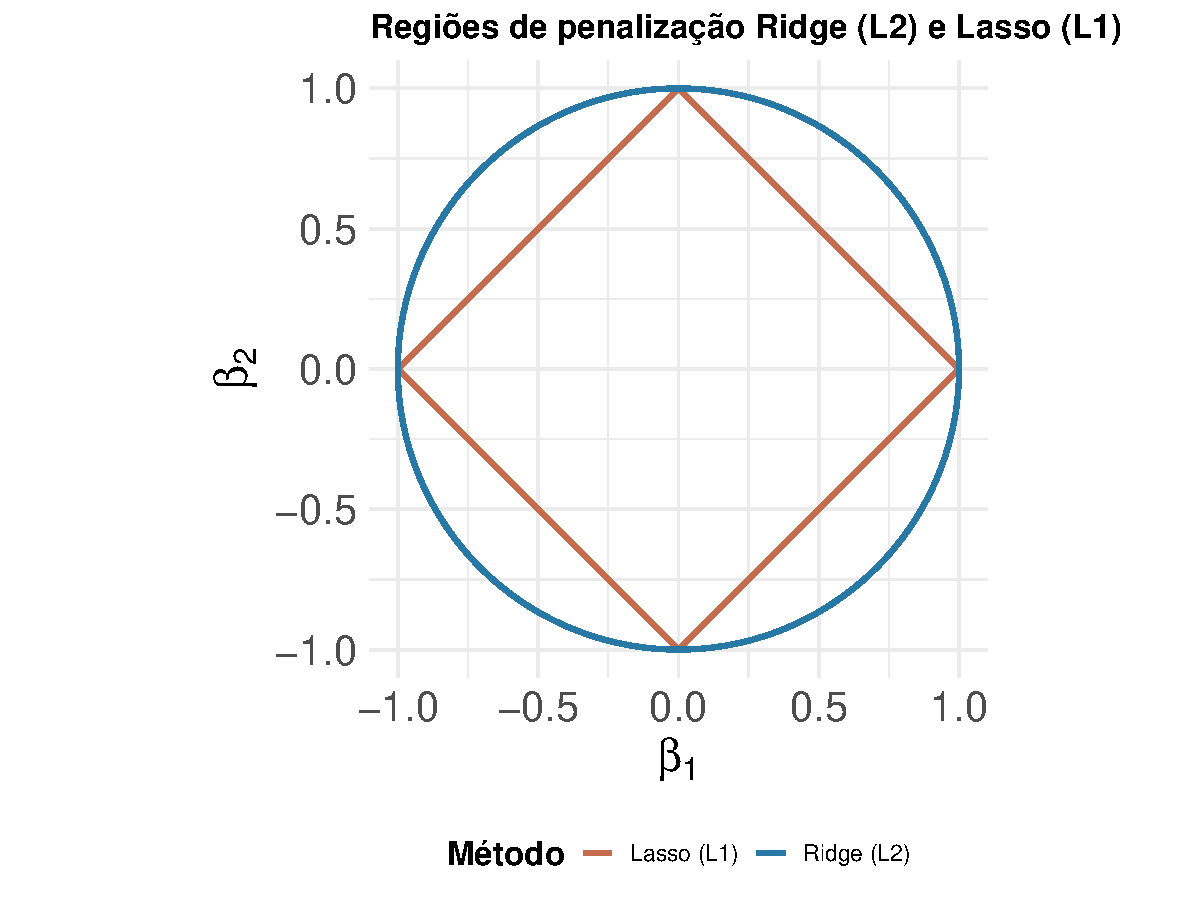
\includegraphics[width=0.7\linewidth,height=\textheight,keepaspectratio]{monografia_v2_files/figure-pdf/fig-regularizacao-1.pdf}

}

\caption{\label{fig-regularizacao}Representação geométrica das regiões
de penalização Ridge (L2) e Lasso (L1). A região circular associada à
penalização L2 tende a reduzir simultaneamente a magnitude dos
coeficientes, enquanto a região em formato de losango da penalização L1
favorece soluções em que alguns coeficientes assumem valor exatamente
igual a zero.}

\end{figure}%

A diferença entre as penalizações L1 e L2 pode ser visualizada
geometricamente na Figura Figura~\ref{fig-regularizacao}. A penalização
Ridge apresenta uma região de restrição circular, enquanto a penalização
Lasso possui uma região em formato de losango. Essa diferença geométrica
está relacionada ao comportamento dos coeficientes durante a estimação:
enquanto a penalização L2 tende a reduzir continuamente a magnitude dos
coeficientes, a penalização L1 favorece soluções em que alguns
parâmetros assumem valores exatamente iguais a zero. Dessa forma, o
Lasso atua também como um método de seleção de variáveis, removendo
preditores com menor contribuição para o modelo.

\subsection{Regressão Logística
Bayesiana}\label{regressuxe3o-loguxedstica-bayesiana}

Enquanto a regressão logística frequentista trata os coeficientes do
modelo como parâmetros fixos e desconhecidos, a abordagem Bayesiana
considera esses parâmetros como variáveis aleatórias. Dessa forma, é
possível incorporar conhecimento prévio sobre os coeficientes por meio
de distribuições \texttt{a\ priori}, que representam as crenças
existentes antes da observação dos dados.

A inferência Bayesiana consiste em combinar essas informações prévias
com a informação contida na amostra, representada pela função de
verossimilhança, obtendo-se a distribuição \texttt{a\ posteriori} dos
parâmetros. Essa distribuição sintetiza o conhecimento atualizado após a
observação dos dados e constitui a base para todas as inferências
realizadas no modelo, como estimação dos coeficientes, construção de
intervalos de credibilidade e obtenção de probabilidades preditivas.

\subsubsection{Formulação do modelo}\label{formulauxe7uxe3o-do-modelo-1}

A estrutura probabilística da regressão logística Bayesiana é a mesma
apresentada para a regressão logística frequentista. Assume-se que a
variável resposta segue uma distribuição de Bernoulli e que sua
probabilidade de ocorrência é relacionada às variáveis explicativas por
meio da função logística aplicada ao preditor linear.

A principal diferença entre as duas abordagens está na forma como os
coeficientes do modelo são tratados. Na abordagem frequentista, os
parâmetros são considerados fixos e desconhecidos, sendo estimados por
máxima verossimilhança. Já na abordagem Bayesiana, os coeficientes são
tratados como variáveis aleatórias e sua inferência é realizada por meio
da distribuição \texttt{a\ posteriori}, obtida pela aplicação do Teorema
de Bayes, conforme apresentado na Seção~\ref{sec-teorema-bayes}.

Dessa forma, enquanto a abordagem frequentista fornece uma estimativa
pontual para cada coeficiente, a regressão logística Bayesiana produz
uma distribuição posterior para cada parâmetro, permitindo quantificar
diretamente a incerteza associada às estimativas e realizar inferências
probabilísticas sobre os coeficientes do modelo.

\subsubsection{\texorpdfstring{Escolha de distribuições \emph{a
priori}}{Escolha de distribuições a priori}}\label{escolha-de-distribuiuxe7uxf5es-a-priori}

Uma das principais características da inferência Bayesiana é a
necessidade de especificar distribuições \emph{a priori} para os
parâmetros do modelo. Essas distribuições representam o conhecimento
disponível sobre os coeficientes antes da observação dos dados e
constituem um dos elementos fundamentais da distribuição posterior.

A escolha da distribuição \emph{a priori} depende tanto do conhecimento
prévio sobre o problema quanto dos objetivos da análise. Em situações
nas quais não há informações prévias relevantes, é comum utilizar
distribuições fracamente informativas, que exercem pouca influência
sobre as estimativas e permitem que a informação proveniente dos dados
tenha maior peso na inferência. Por outro lado, quando existe
conhecimento substancial sobre os parâmetros ou quando se deseja
incorporar algum tipo de regularização, podem ser utilizadas
distribuições com características específicas, capazes de induzir
diferentes comportamentos nas estimativas.

Além de representar conhecimento prévio, as distribuições \emph{a
priori} desempenham um papel importante na regularização dos modelos
Bayesianos. Dependendo da distribuição adotada, pode-se favorecer
coeficientes de menor magnitude, reduzir os efeitos da
multicolinearidade ou incentivar a seleção automática de variáveis.
Dessa forma, a escolha da priori influencia não apenas a inferência
estatística, mas também a complexidade e a interpretabilidade do modelo.

\paragraph{Priori Normal}\label{priori-normal}

Uma das distribuições \emph{a priori} mais utilizadas em regressão
logística Bayesiana é a distribuição Normal. Nessa abordagem, assume-se
que cada coeficiente do modelo é proveniente de uma distribuição Normal
centrada em um valor esperado, geralmente igual a zero:

\begin{equation}\protect\phantomsection\label{eq-prior-normal}{
\beta_j
\sim
\mathcal{N}
(\mu,\sigma^2)
}\end{equation}

Na maioria das aplicações, adota-se \(\mu=0\), refletindo a expectativa
de que, antes da observação dos dados, não exista evidência de que
determinada variável exerça efeito positivo ou negativo sobre a
resposta. O parâmetro \(\sigma^2\) controla o grau de dispersão da
distribuição e, consequentemente, a intensidade da informação prévia
incorporada ao modelo.

Valores elevados de \(\sigma\) produzem distribuições mais dispersas,
permitindo que a informação proveniente dos dados exerça maior
influência sobre a distribuição posterior. Por outro lado, valores
reduzidos concentram maior massa de probabilidade em torno de zero,
favorecendo coeficientes de menor magnitude e restringindo estimativas
extremas. Assim, quanto menor o desvio padrão adotado, maior a
intensidade da regularização imposta aos parâmetros.

\begin{figure}

\centering{

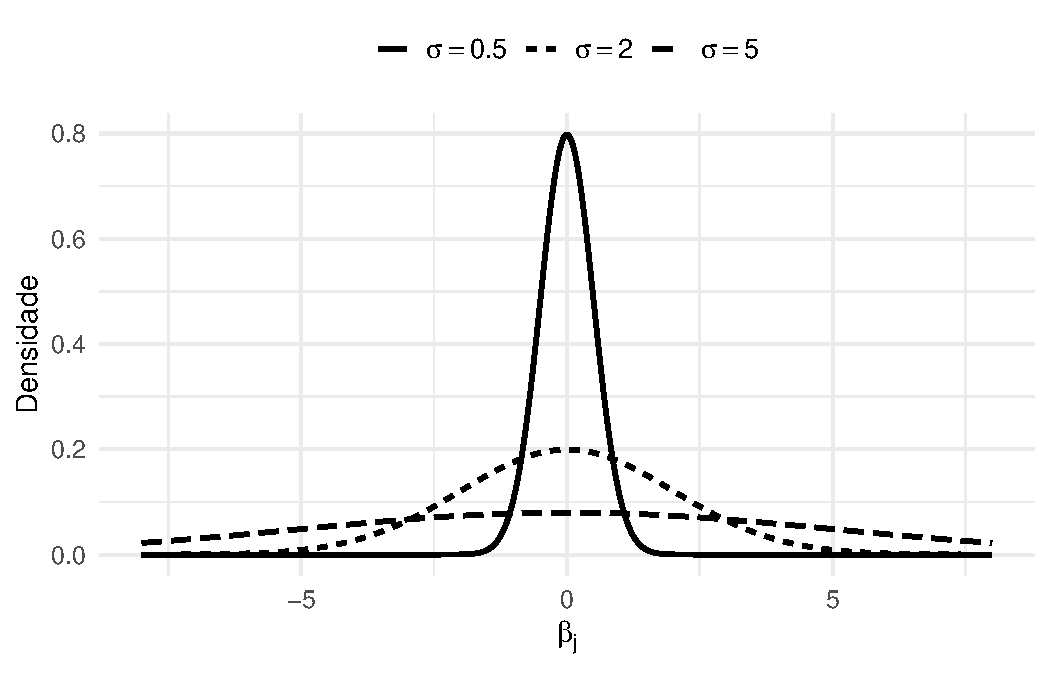
\includegraphics[width=0.75\linewidth,height=\textheight,keepaspectratio]{monografia_v2_files/figure-pdf/fig-prior-normal-1.pdf}

}

\caption{\label{fig-prior-normal}Distribuições Normais a priori com
diferentes desvios padrão.}

\end{figure}%

A influência do desvio padrão sobre a distribuição \emph{a priori} pode
ser observada na Figura Figura~\ref{fig-prior-normal}. Valores menores
de \(\sigma\) concentram maior massa de probabilidade em torno de zero,
tornando menos prováveis coeficientes de grande magnitude e aumentando a
intensidade da regularização. À medida que o desvio padrão aumenta, a
distribuição torna-se mais dispersa, permitindo que os dados exerçam
maior influência sobre as estimativas posteriores.

A utilização de uma distribuição Normal como priori estabelece uma
relação direta com a regularização Ridge utilizada na abordagem
frequentista. Na regressão Ridge, a estimação dos coeficientes é
realizada maximizando a função de verossimilhança penalizada, dada pela
Equação~\ref{eq-ridge}.

Por sua vez, ao assumir uma distribuição \emph{a priori} Normal,

\[
\beta_j
\sim
\mathcal{N}
(0,\sigma^2),
\]

o logaritmo da densidade da priori pode ser escrito, desprezando
constantes, como:

\begin{equation}\protect\phantomsection\label{eq-logprior-normal}{
\log p(\beta)
\propto
-
\frac{1}{2\sigma^2}
\sum_{j=1}^{p}
\beta_j^2.
}\end{equation}

Observa-se que tanto a penalização Ridge quanto o logaritmo da priori
Normal contêm um termo quadrático envolvendo os coeficientes do modelo.
Assim, embora provenientes de interpretações distintas, uma baseada em
penalização e outra na incorporação de uma distribuição
\texttt{a\ priori}, ambas favorecem coeficientes de menor magnitude. A
principal diferença reside na interpretação: na regressão Ridge, o termo
quadrático é introduzido como uma penalização na função objetivo,
enquanto na abordagem Bayesiana ele decorre da escolha da distribuição
\texttt{a\ priori} para os parâmetros.

Nota-se que existe uma relação inversa entre os parâmetros de
regularização: valores menores de \(\sigma^2\) correspondem a uma priori
mais concentrada em torno de zero e, consequentemente, a uma
regularização mais intensa, desempenhando papel análogo ao parâmetro de
penalização \(\lambda\) da regressão Ridge. Assim, reduzir \(\sigma^2\)
equivale a aumentar a intensidade da regularização.

Assim como a penalização Ridge, a priori Normal reduz a magnitude dos
coeficientes estimados, mas não realiza seleção automática de variáveis,
uma vez que os parâmetros tendem a permanecer diferentes de zero após a
estimação.

\paragraph{Priori Laplace}\label{priori-laplace}

Outra distribuição \emph{a priori} amplamente utilizada em regressão
logística Bayesiana é a distribuição Laplace, também conhecida como
distribuição de dupla exponencial (\emph{double exponential}).
Diferentemente da distribuição Normal, a distribuição Laplace apresenta
um pico mais acentuado em torno de zero e caudas mais pesadas,
favorecendo coeficientes pequenos sem restringir completamente a
ocorrência de valores de maior magnitude.

Matematicamente, a priori Laplace pode ser representada por:

\begin{equation}\protect\phantomsection\label{eq-prior-laplace}{
\beta_j
\sim
\text{Laplace}
(\mu,b)
}\end{equation}

Em geral, adota-se \(\mu=0\), indicando que, antes da observação dos
dados, espera-se que os coeficientes estejam concentrados em torno de
zero. O parâmetro \(b\) controla a dispersão da distribuição: valores
menores de \(b\) concentram maior massa de probabilidade em torno de
zero, intensificando a regularização, enquanto valores maiores tornam a
distribuição mais dispersa e reduzem a influência da informação prévia.

\begin{figure}

\centering{

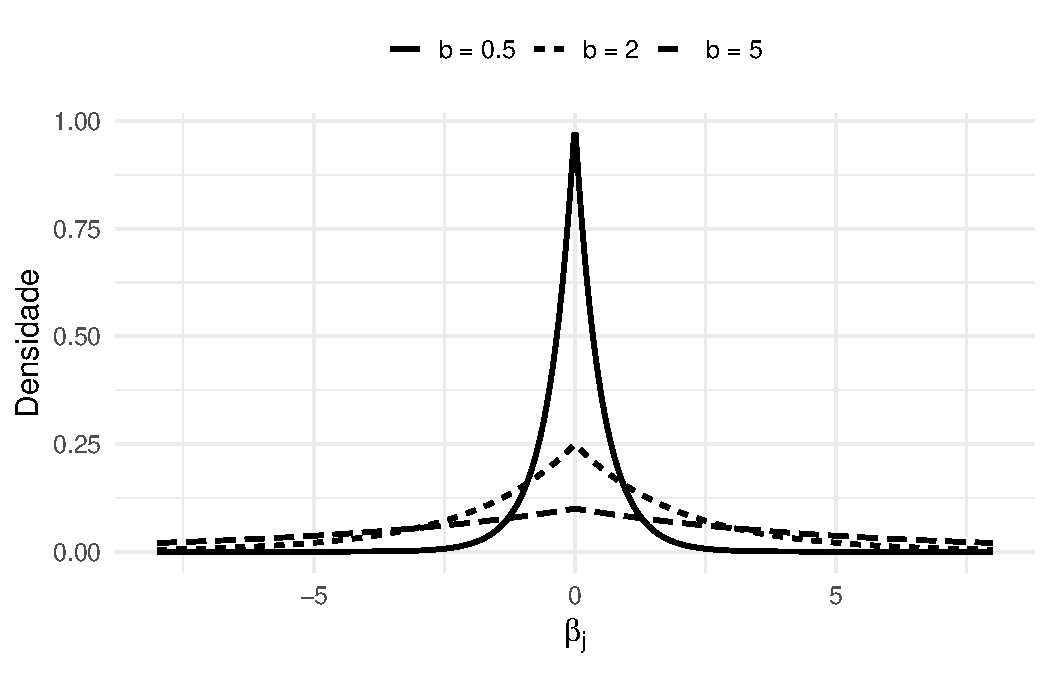
\includegraphics[width=0.75\linewidth,height=\textheight,keepaspectratio]{monografia_v2_files/figure-pdf/fig-prior-laplace-1.pdf}

}

\caption{\label{fig-prior-laplace}Distribuições Laplace a priori com
diferentes parâmetros de escala.}

\end{figure}%

A Figura Figura~\ref{fig-prior-laplace} ilustra o efeito do parâmetro
\(b\) sobre a distribuição Laplace. À medida que \(b\) diminui, a
distribuição torna-se mais concentrada em torno de zero, aumentando a
probabilidade de coeficientes com pequena magnitude. Em contrapartida,
suas caudas permanecem relativamente pesadas quando comparadas às da
distribuição Normal, permitindo que coeficientes com efeitos realmente
relevantes assumam valores mais elevados quando sustentados pelos dados.

A utilização da distribuição Laplace estabelece uma relação direta com a
regularização Lasso empregada na abordagem frequentista. Enquanto o
Lasso adiciona uma penalização baseada na soma dos valores absolutos dos
coeficientes, conforme apresentado na Equação~\ref{eq-lasso}, o
logaritmo da densidade da distribuição Laplace pode ser escrito,
desprezando constantes, como

\begin{equation}\protect\phantomsection\label{eq-logprior-laplace}{
\log p(\beta)
\propto
-
\frac{1}{b}
\sum_{j=1}^{p}
|\beta_j|.
}\end{equation}

Observa-se que ambas as expressões apresentam um termo baseado no valor
absoluto dos coeficientes. Assim, embora provenientes de interpretações
distintas, uma decorrente de uma penalização e outra da especificação de
uma distribuição \emph{a priori}, ambas favorecem soluções mais esparsas
(\emph{sparse}), nas quais apenas parte das variáveis apresenta efeitos
relevantes.

Assim como a regularização Lasso, a priori Laplace promove um
encolhimento mais intenso dos coeficientes em direção a zero do que a
distribuição Normal. Como consequência, tende a produzir modelos mais
parcimoniosos, reduzindo a influência de variáveis com pouca
contribuição para a resposta e facilitando a interpretação do modelo.

\paragraph{\texorpdfstring{Sensibilidade às distribuições \emph{a
priori}}{Sensibilidade às distribuições a priori}}\label{sensibilidade-uxe0s-distribuiuxe7uxf5es-a-priori}

Uma etapa importante da modelagem Bayesiana consiste em avaliar a
sensibilidade dos resultados à escolha das distribuições \emph{a
priori}. Como a distribuição posterior é obtida pela combinação entre a
priori e a verossimilhança, diferentes especificações podem produzir
estimativas distintas, especialmente em situações com amostras reduzidas
ou baixa quantidade de informação nos dados.

Em geral, quando o conjunto de dados é suficientemente informativo,
espera-se que pequenas alterações nas distribuições \emph{a priori}
tenham impacto limitado sobre as estimativas posteriores. Por outro
lado, diferenças substanciais entre os resultados obtidos com diferentes
prioris podem indicar que as inferências são fortemente influenciadas
pelas hipóteses iniciais adotadas.

\subsubsection{\texorpdfstring{Distribuições \emph{a
posteriori}}{Distribuições a posteriori}}\label{distribuiuxe7uxf5es-a-posteriori}

Na inferência Bayesiana, a distribuição \emph{a posteriori} dos
parâmetros é obtida pela combinação entre a distribuição \emph{a priori}
e a função de verossimilhança, conforme estabelecido pelo Teorema de
Bayes (Seção~\ref{sec-teorema-bayes}). Enquanto a distribuição \emph{a
priori} representa o conhecimento ou as suposições estabelecidas sobre
os parâmetros antes da observação dos dados, a verossimilhança incorpora
a informação fornecida pela amostra observada. Dessa forma, a
distribuição \emph{a posteriori} expressa o conhecimento atualizado
sobre os parâmetros após considerar as evidências disponíveis.

Formalmente, a distribuição \emph{a posteriori} pode ser expressa por:

\begin{equation}\protect\phantomsection\label{eq-posterior}{
p(\beta \mid y, X)
=
\frac{
p(y \mid X, \beta)\,p(\beta)
}{
p(y \mid X)
}
}\end{equation}

em que \(p(\beta \mid y, X)\) representa a distribuição \emph{a
posteriori} dos parâmetros; \(p(y \mid X, \beta)\) corresponde à função
de verossimilhança; \(p(\beta)\) representa a distribuição \emph{a
priori}; e \(p(y \mid X)\) é a distribuição marginal dos dados, também
denominada constante de normalização.

Neste contexto, \(X\) representa a matriz de variáveis explicativas,
composta pelas características observadas dos indivíduos, enquanto \(y\)
corresponde ao vetor de observações da variável resposta. O vetor
\(\beta\) contém os parâmetros do modelo de regressão logística a serem
estimados.

Como o denominador não depende dos parâmetros, a distribuição \emph{a
posteriori} pode ser expressa proporcionalmente ao produto entre a
verossimilhança e a distribuição \emph{a priori}:

\begin{equation}\protect\phantomsection\label{eq-posterior-proporcional}{
p(\beta \mid y, X)
\propto
p(y \mid X, \beta)
p(\beta).
}\end{equation}

Essa relação evidencia que a inferência Bayesiana não considera apenas a
informação observada nos dados, mas também as suposições estabelecidas
previamente sobre os parâmetros. A influência relativa de cada
componente depende, entre outros fatores, da quantidade de informação
presente na amostra e da dispersão atribuída às distribuições \emph{a
priori}.

Na regressão logística, a distribuição \emph{a priori} é especificada
para os coeficientes do modelo, representados por \(\beta\). Esses
parâmetros determinam a relação entre as variáveis explicativas e a
probabilidade de ocorrência do evento de interesse. Antes de observar os
dados, a distribuição \emph{a priori} estabelece quais valores desses
coeficientes são considerados mais ou menos plausíveis. Após a
observação da amostra, a função de verossimilhança incorpora as
informações fornecidas pelos dados, atribuindo maior suporte aos valores
dos parâmetros que resultam em probabilidades mais compatíveis com os
resultados observados.

A distribuição \emph{a posteriori} surge, portanto, da combinação dessas
duas fontes de informação. Para compreender esse processo, pode-se
considerar que a distribuição \emph{a priori} representa uma
distribuição inicial de plausibilidade dos parâmetros, enquanto a
verossimilhança atua como um mecanismo de atualização, modificando essa
distribuição de acordo com a evidência empírica. Assim, valores dos
parâmetros que recebem maior suporte tanto da distribuição \emph{a
priori} quanto da verossimilhança tendem a apresentar maior concentração
de probabilidade na distribuição \emph{a posteriori}.

Essa atualização não corresponde simplesmente à substituição da
distribuição \emph{a priori} pelas estimativas obtidas a partir dos
dados. Em vez disso, a distribuição \emph{a posteriori} preserva a
influência da informação prévia, combinando-a com a evidência observada.
A intensidade dessa influência depende da compatibilidade entre as
informações fornecidas pela priori e pela verossimilhança, bem como da
quantidade de informação disponível na amostra e da dispersão atribuída
à distribuição \emph{a priori}.

\begin{figure}

\centering{

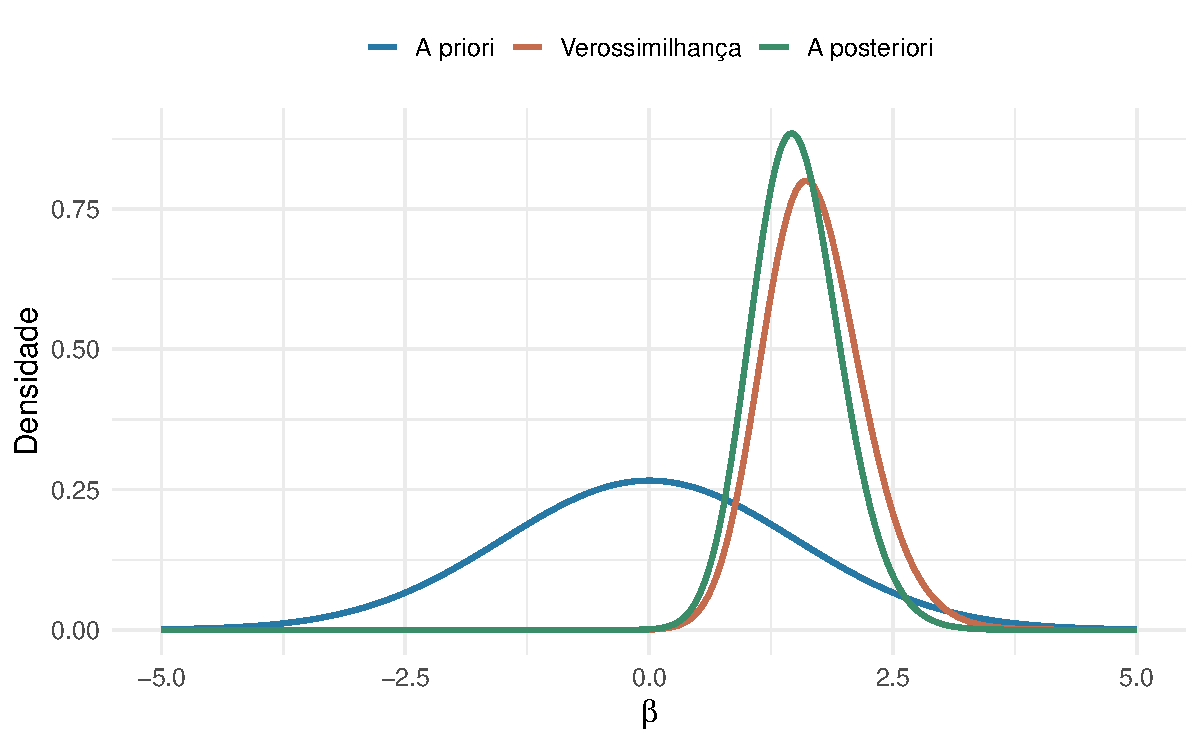
\includegraphics[width=0.75\linewidth,height=\textheight,keepaspectratio]{monografia_v2_files/figure-pdf/fig-atualizacao-bayesiana-1.pdf}

}

\caption{\label{fig-atualizacao-bayesiana}Representação da atualização
Bayesiana em um modelo de regressão logística: distribuição a priori,
verossimilhança normalizada e distribuição a posteriori.}

\end{figure}%

Para ilustrar o processo de atualização bayesiana, considere um exemplo
hipotético em que são observadas 25 ocorrências de um determinado evento
em uma amostra de 30 observações. Suponha, inicialmente, que o
coeficiente associado a esse evento siga uma distribuição \emph{a
priori} Normal, com média zero e desvio-padrão igual a 1,5. Essa
especificação expressa uma expectativa inicial de que o efeito seja
próximo de zero, embora permita valores positivos e negativos.

A partir dos dados observados, a função de verossimilhança passa a
favorecer valores positivos do coeficiente, uma vez que a proporção de
ocorrências na amostra é relativamente elevada. Ao combinar essa
informação com a distribuição \emph{a priori}, obtém-se a distribuição
\emph{a posteriori}, que representa a atualização do conhecimento sobre
o parâmetro após a observação dos dados.

Como ilustrado na Figura~\ref{fig-atualizacao-bayesiana}, a distribuição
\emph{a posteriori} apresenta uma posição intermediária entre a
distribuição \emph{a priori} e a verossimilhança normalizada. Esse
resultado evidencia que a inferência bayesiana não considera
exclusivamente os dados observados, tampouco mantém inalterada a
expectativa inicial: a distribuição \emph{a posteriori} resulta da
combinação dessas duas fontes de informação.

\begin{figure}

\centering{

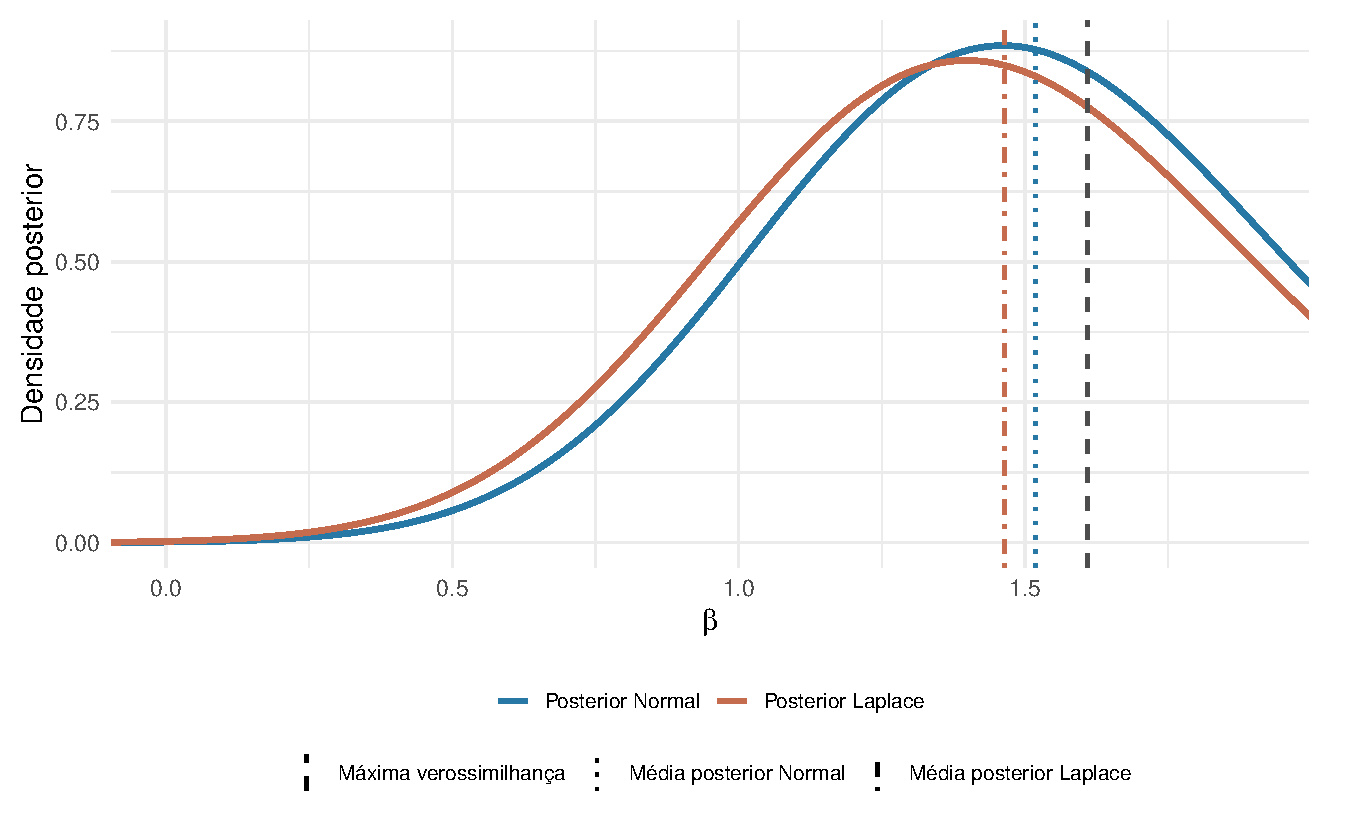
\includegraphics[width=0.9\linewidth,height=\textheight,keepaspectratio]{monografia_v2_files/figure-pdf/fig-shrinkage-1.pdf}

}

\caption{\label{fig-shrinkage}Distribuições posteriores e contração das
estimativas em relação à máxima verossimilhança, sob priors Normal e
Laplace.}

\end{figure}%

A influência da distribuição \emph{a priori} não se limita à atualização
da informação sobre os parâmetros, podendo também afetar a magnitude das
estimativas posteriores por meio de um mecanismo de regularização
denominado \emph{shrinkage}. Esse fenômeno corresponde à contração dos
coeficientes em direção aos valores favorecidos pela distribuição
\emph{a priori}. Quando centrada em zero, essa distribuição tende a
favorecer estimativas de menor magnitude, sendo a intensidade da
contração determinada, entre outros fatores, por sua forma e dispersão.
Conforme ilustrado na Figura~\ref{fig-shrinkage}, a incorporação de
distribuições \emph{a priori} centradas em zero pode deslocar as
estimativas posteriores em direção a esse valor, em comparação com a
estimativa de máxima verossimilhança. Nesse contexto, diferentes
especificações podem produzir comportamentos distintos: enquanto a
distribuição Normal promove uma regularização mais suave, a distribuição
Laplace apresenta maior concentração de probabilidade nas proximidades
de zero e caudas mais pesadas, podendo favorecer uma contração mais
acentuada de coeficientes de menor magnitude.

A comparação entre essas distribuições permite investigar como
diferentes estruturas de informação prévia influenciam as estimativas
dos parâmetros e a incerteza posterior. Cabe destacar, entretanto, que a
contração dos coeficientes não implica necessariamente que sejam
estimados exatamente como zero. Assim, embora a distribuição Laplace
possa favorecer estimativas próximas de zero, sua utilização como
distribuição \emph{a priori} não corresponde, por si só, à seleção
automática de variáveis.

\subsubsection{Inferência via MCMC}\label{inferuxeancia-via-mcmc}

Embora a distribuição \emph{a posteriori} seja definida matematicamente
pela combinação entre a distribuição \emph{a priori} e a função de
verossimilhança, sua obtenção analítica nem sempre é possível. Em
modelos de regressão logística com múltiplas variáveis explicativas, a
integração necessária para determinar a constante de normalização da
distribuição \emph{a posteriori} geralmente não possui solução fechada.
Consequentemente, torna-se necessário recorrer a métodos computacionais
para aproximar essa distribuição.

Neste trabalho, a inferência Bayesiana é realizada por meio de métodos
de Monte Carlo via Cadeias de Markov (\emph{Markov Chain Monte Carlo},
MCMC), implementados pela biblioteca \texttt{rstanarm} do R, que utiliza
o Stan como mecanismo de estimação. Esses métodos permitem obter
amostras da distribuição \emph{a posteriori} por meio da construção de
cadeias de Markov cuja distribuição estacionária corresponde à
distribuição de interesse.

Diferentemente da abordagem frequentista, que geralmente apresenta
estimativas pontuais para os parâmetros, os métodos MCMC permitem
representar a incerteza associada às estimativas por meio de uma amostra
da distribuição \emph{a posteriori}. A partir dessas amostras, podem ser
calculadas medidas como médias, medianas, desvios padrão, intervalos de
credibilidade e probabilidades posteriores, proporcionando uma descrição
mais completa da incerteza sobre os parâmetros do modelo.

Na prática, o procedimento utiliza múltiplas cadeias de Markov,
iniciadas em diferentes valores dos parâmetros. Antes da etapa de
amostragem utilizada para a inferência, realiza-se um período inicial
denominado \emph{warm-up}, durante o qual o algoritmo adapta
determinados parâmetros internos para melhorar a eficiência da
amostragem. As iterações dessa etapa são descartadas e não são
utilizadas no cálculo dos resumos da distribuição \emph{a posteriori}.

Após o período de \emph{warm-up}, são geradas as amostras utilizadas
para representar a distribuição \emph{a posteriori}. A qualidade dessas
amostras depende da convergência das cadeias e da eficiência com que
exploram o espaço paramétrico. Por esse motivo, torna-se necessário
avaliar os resultados por meio de diagnósticos específicos, como o fator
de redução potencial de escala (\(\hat{R}\)), o tamanho efetivo da
amostra (ESS), a inspeção gráfica das trajetórias das cadeias e os
diagnósticos associados ao algoritmo Hamiltoniano de Monte Carlo
(\emph{Hamiltonian Monte Carlo}, HMC).

Além de permitir que as cadeias alcancem regiões de maior probabilidade
da distribuição \emph{a posteriori}, essa etapa é utilizada para ajustar
automaticamente parâmetros internos do algoritmo, como o tamanho do
passo (\emph{step size}) e a matriz de massa (\emph{mass matrix}),
tornando a amostragem posterior mais eficiente.

Por exemplo, ao executar quatro cadeias com 2.000 iterações cada, sendo
as primeiras 1.000 destinadas ao \emph{warm-up}, apenas as 1.000
iterações finais de cada cadeia são utilizadas para a inferência,
resultando em um total de 4.000 amostras da distribuição \emph{a
posteriori}.

Adicionalmente, a precisão das estimativas obtidas por meio das amostras
simuladas pode ser avaliada pelo erro-padrão de Monte Carlo (\emph{Monte
Carlo Standard Error}, MCSE). Essa medida quantifica a incerteza
numérica decorrente do número finito de amostras utilizadas para
aproximar as quantidades de interesse da distribuição \emph{a
posteriori}, considerando também a autocorrelação entre as realizações
da cadeia. Valores menores de MCSE indicam maior precisão numérica das
estimativas, embora sua interpretação deva considerar a escala e a
magnitude da quantidade estimada. Diferentemente do fator \(\hat{R}\),
que auxilia na avaliação da convergência das cadeias, e do ESS, que
mensura a quantidade efetiva de informação disponível nas amostras, o
MCSE permite avaliar a precisão das estimativas Monte Carlo.

O Stan implementa, por padrão, o algoritmo \emph{No-U-Turn Sampler}
(NUTS), uma extensão adaptativa do HMC. Ambos pertencem à família MCMC,
cujo objetivo é gerar amostras da distribuição \emph{a posteriori} dos
parâmetros.

Em algoritmos clássicos de MCMC, como o Metropolis-Hastings, novas
propostas são geradas por pequenos deslocamentos aleatórios em torno da
posição atual da cadeia. Embora esse procedimento seja conceitualmente
simples, ele tende a explorar a distribuição de forma lenta, produzindo
amostras altamente correlacionadas e exigindo um grande número de
iterações para representar adequadamente a distribuição \emph{a
posteriori}.

O Hamiltonian Monte Carlo busca contornar essa limitação utilizando o
gradiente do logaritmo da distribuição a posteriori. Essa informação
indica como a densidade varia localmente e é utilizada para construir
trajetórias que percorrem a distribuição de maneira eficiente, evitando
os pequenos movimentos aleatórios característicos de métodos como o
Metropolis-Hastings. Dessa forma, a cadeia consegue explorar regiões de
alta probabilidade com deslocamentos mais longos, produzindo amostras
menos correlacionadas e acelerando a convergência.

Para construir essas trajetórias, o HMC utiliza conceitos da Mecânica
Hamiltoniana, tratando os parâmetros do modelo como se fossem partículas
em movimento sob a ação de forças. Embora essa interpretação seja
física, sua principal utilidade é fornecer um mecanismo eficiente para
explorar distribuições de alta dimensão preservando suas propriedades
probabilísticas.

Apesar dessas vantagens, o desempenho do HMC depende da escolha de
alguns hiperparâmetros, principalmente o tamanho do passo (\emph{step
size}) e o número de passos utilizados para percorrer cada trajetória.
Valores inadequados podem tornar a exploração ineficiente ou aumentar
significativamente o custo computacional.

O algoritmo NUTS (\emph{No-U-Turn Sampler}) elimina grande parte dessa
dificuldade ao adaptar automaticamente o comprimento das trajetórias
durante a amostragem. Em vez de definir previamente quantos passos devem
ser executados, o algoritmo expande a trajetória até identificar que ela
começou a retornar em direção ao ponto de partida, formando um movimento
semelhante a um ``U''. Nesse momento, a trajetória é interrompida,
evitando que o algoritmo desperdice iterações percorrendo repetidamente
a mesma região da distribuição.

Essa estratégia permite que o Stan explore automaticamente a
distribuição \emph{a posteriori} de forma eficiente, reduzindo a
necessidade de ajustes manuais e tornando o método adequado para modelos
Bayesianos complexos e de alta dimensão.

Ao final da amostragem, obtém-se um conjunto de realizações da
distribuição \emph{a posteriori} para cada parâmetro do modelo. Essas
amostras constituem a base para todas as inferências realizadas na
abordagem Bayesiana, incluindo a estimação dos coeficientes, a
construção de intervalos de credibilidade e a avaliação da incerteza
associada às previsões.

\paragraph{Diagnóstico da
convergência}\label{diagnuxf3stico-da-converguxeancia}

Após a obtenção das amostras da distribuição \emph{a posteriori}, é
necessário verificar se o processo de amostragem convergiu
adequadamente. A convergência indica que as cadeias de Markov passaram a
representar a mesma distribuição \emph{a posteriori}, permitindo que as
inferências realizadas sejam consideradas confiáveis. Entre os
principais diagnósticos utilizados destacam-se os \emph{traceplots}, o
fator de redução potencial (\(\hat{R}\)) e o tamanho efetivo da amostra
(\emph{Effective Sample Size}, ESS).

Os \emph{traceplots} consistem em gráficos que apresentam os valores
amostrados para cada parâmetro ao longo das iterações do algoritmo.
Espera-se que, após o período de \emph{warm-up}, as diferentes cadeias
apresentem boa mistura (mixing), alternando-se livremente em torno da
mesma região da distribuição a posteriori. Esse comportamento sugere que
a cadeia está explorando adequadamente a distribuição \emph{a
posteriori}. Por outro lado, padrões como tendências persistentes,
mudanças abruptas ou cadeias que permanecem separadas podem indicar
problemas de convergência.

A Figura~\ref{fig-traceplots} ilustra dois comportamentos típicos. À
esquerda observa-se uma situação de convergência, em que as cadeias
apresentam boa mistura (mixing) e exploram a mesma região da
distribuição a posteriori. À direita, as cadeias permanecem separadas e
apresentam comportamento não estacionário, indicando que a convergência
ainda não foi atingida.

\begin{figure}

\centering{

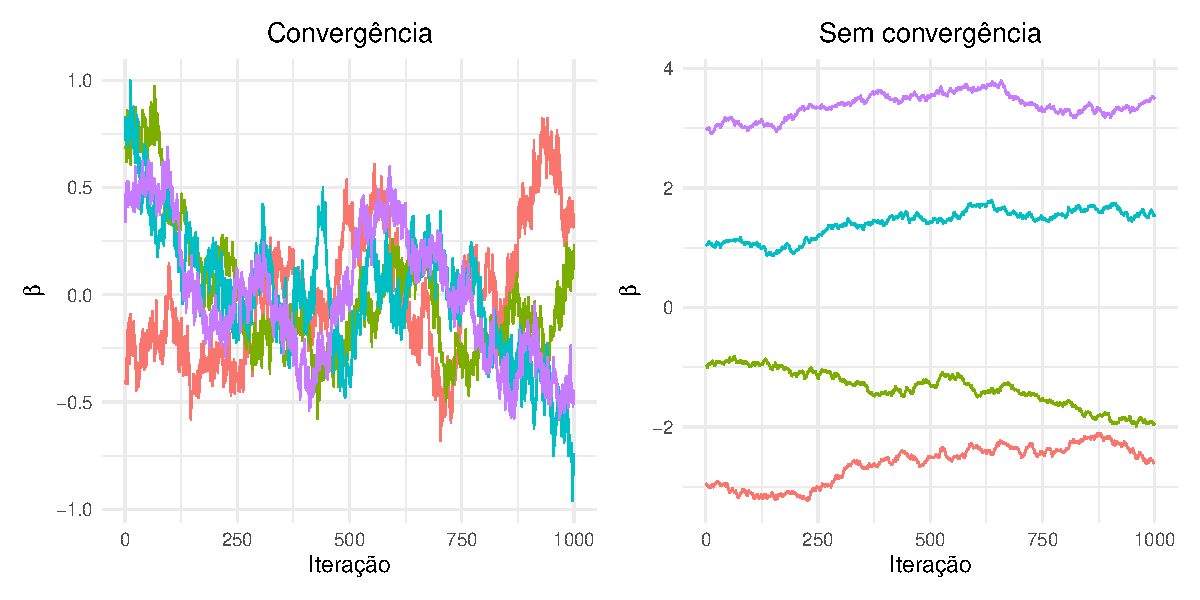
\includegraphics[width=0.9\linewidth,height=\textheight,keepaspectratio]{monografia_v2_files/figure-pdf/fig-traceplots-1.pdf}

}

\caption{\label{fig-traceplots}Exemplo ilustrativo de traceplots. À
esquerda, cadeias convergidas apresentam boa mistura e exploram a mesma
distribuição posterior. À direita, cadeias não convergidas permanecem
separadas, indicando problemas de convergência.}

\end{figure}%

O fator de redução potencial, denotado por (\(\hat{R}\)) e proposto por
Gelman e Rubin, compara a variabilidade entre diferentes cadeias com a
variabilidade observada dentro de cada cadeia. Quando todas as cadeias
convergem para a mesma distribuição, espera-se que essas variabilidades
sejam semelhantes, resultando em valores de (\(\hat{R}\)) próximos de 1.
Na prática, valores inferiores a 1,01 são geralmente considerados
indicativos de boa convergência.

Outro diagnóstico importante é o tamanho efetivo da amostra
(\emph{Effective Sample Size}, ESS). Embora um algoritmo MCMC possa
gerar milhares de amostras, elas não são independentes, pois observações
consecutivas tendem a apresentar autocorrelação. O ESS estima quantas
amostras independentes seriam equivalentes ao conjunto obtido pelo
algoritmo. Assim, valores elevados de ESS indicam que a distribuição
\emph{a posteriori} foi explorada de forma eficiente, enquanto valores
reduzidos sugerem elevada autocorrelação e a necessidade de aumentar o
número de iterações ou investigar possíveis problemas na amostragem.

Adicionalmente, o diagnóstico E-BFMI (Energy Bayesian Fraction of
Missing Information) avalia a eficiência da exploração da distribuição
de energia pelo algoritmo Hamiltoniano, permitindo identificar possíveis
dificuldades na exploração do espaço paramétrico. Valores reduzidos
podem indicar problemas na amostragem e a necessidade de investigar a
parametrização do modelo ou as configurações do algoritmo.

Neste trabalho, esses diagnósticos foram utilizados conjuntamente para
avaliar a convergência das cadeias e a eficiência da amostragem
realizada pelo algoritmo NUTS.

\paragraph{Inferência posterior}\label{inferuxeancia-posterior}

Uma vez verificada a convergência das cadeias, as amostras geradas pelo
algoritmo MCMC passam a representar a distribuição \emph{a posteriori}
de cada parâmetro do modelo. Diferentemente da abordagem frequentista,
em que a inferência é baseada em uma única estimativa pontual dos
coeficientes, a abordagem Bayesiana considera toda a distribuição
posterior, permitindo quantificar diretamente a incerteza associada às
estimativas.

Uma medida frequentemente utilizada para resumir essa distribuição é a
média posterior, obtida pela média das amostras geradas para cada
parâmetro. Essa quantidade representa o valor esperado do coeficiente
após a incorporação simultânea das informações provenientes da
distribuição \emph{a priori} e dos dados observados.

Além da média posterior, é comum apresentar intervalos de credibilidade,
que descrevem a região da distribuição \emph{a posteriori} onde se
concentram os valores mais plausíveis para cada parâmetro. Um intervalo
de credibilidade de 95\% indica que, dadas as distribuições \emph{a
priori} adotadas e os dados observados, existe uma probabilidade de 95\%
de que o verdadeiro valor do parâmetro pertença ao intervalo obtido.

Em aplicações práticas, também é comum avaliar se o intervalo de
credibilidade de um coeficiente contém o valor zero. Quando todo o
intervalo permanece acima ou abaixo de zero, há evidências de que o
efeito da variável seja predominantemente positivo ou negativo,
respectivamente

Essa interpretação difere dos intervalos de confiança utilizados na
estatística frequentista. Enquanto o intervalo de confiança está
relacionado ao comportamento do procedimento de estimação em repetições
hipotéticas do experimento, o intervalo de credibilidade permite fazer
afirmações probabilísticas diretamente sobre o parâmetro de interesse.

A interpretação dos coeficientes permanece análoga à da regressão
logística frequentista. Cada coeficiente representa a variação esperada
no logaritmo das chances (\emph{log-odds}) associada ao aumento de uma
unidade da variável explicativa, mantendo-se constantes as demais
variáveis do modelo.

\paragraph{Avaliação do modelo
Bayesiano}\label{avaliauxe7uxe3o-do-modelo-bayesiano}

Além dos diagnósticos de convergência das cadeias e da interpretação dos
parâmetros, modelos bayesianos permitem avaliar sua adequação e
capacidade preditiva por meio de critérios baseados na distribuição
preditiva posterior.

A verificação preditiva posterior (\emph{Posterior Predictive Check},
PPC) compara características dos dados observados com aquelas obtidas em
replicações simuladas a partir do modelo. Essa análise permite avaliar
se o modelo consegue reproduzir aspectos relevantes dos dados utilizados
no ajuste.

Outro critério é o \emph{Widely Applicable Information Criterion}
(WAIC), que estima a capacidade preditiva esperada do modelo,
considerando a incerteza dos parâmetros e penalizando sua complexidade
efetiva. O WAIC está relacionado à \emph{Expected Log Predictive
Density} (ELPD), medida da qualidade preditiva esperada para novas
observações, cuja estimativa pode ser obtida a partir dos dados
disponíveis.

Neste trabalho, o PPC é utilizado para avaliar a adequação dos modelos
bayesianos aos dados observados, enquanto o WAIC é empregado como
critério complementar de comparação entre diferentes especificações
bayesianas. Já as métricas tradicionais de classificação permitem
comparar diretamente os modelos frequentistas e bayesianos.

\subsection{Avaliação de modelos de
classificação}\label{avaliauxe7uxe3o-de-modelos-de-classificauxe7uxe3o}

A avaliação de modelos de classificação binária pode ser realizada por
diferentes métricas, cada uma enfatizando um aspecto distinto do
desempenho do modelo. Em problemas de concessão de crédito, essa
avaliação torna-se particularmente importante, uma vez que diferentes
tipos de erro possuem impactos econômicos distintos para a instituição
financeira. Dessa forma, a análise do desempenho não deve se restringir
a uma única medida, sendo recomendável a utilização de um conjunto de
métricas obtidas a partir da matriz de confusão. As métricas abaixo são
utilizadas em ambas as abordagens, frequentista e Bayesiana, permitindo
comparar o desempenho dos modelos sob diferentes perspectivas.

\subsubsection{Matriz de confusão}\label{matriz-de-confusuxe3o}

A matriz de confusão resume a relação entre as classes observadas e as
classes previstas pelo modelo, permitindo identificar a quantidade de
classificações corretas e incorretas. Para um problema de classificação
binária, ela é composta por quatro elementos:

{\def\LTcaptype{none} % do not increment counter
\begin{longtable}[]{@{}
  >{\raggedright\arraybackslash}p{(\linewidth - 4\tabcolsep) * \real{0.2727}}
  >{\raggedleft\arraybackslash}p{(\linewidth - 4\tabcolsep) * \real{0.3636}}
  >{\raggedleft\arraybackslash}p{(\linewidth - 4\tabcolsep) * \real{0.3636}}@{}}
\toprule\noalign{}
\begin{minipage}[b]{\linewidth}\raggedright
\end{minipage} & \begin{minipage}[b]{\linewidth}\raggedleft
Classe prevista: Positiva
\end{minipage} & \begin{minipage}[b]{\linewidth}\raggedleft
Classe prevista: Negativa
\end{minipage} \\
\midrule\noalign{}
\endhead
\bottomrule\noalign{}
\endlastfoot
\textbf{Classe observada: Positiva} & Verdadeiro Positivo (TP) & Falso
Negativo (FN) \\
\textbf{Classe observada: Negativa} & Falso Positivo (FP) & Verdadeiro
Negativo (TN) \\
\end{longtable}
}

A partir desses quatro valores, diversas métricas podem ser calculadas
para avaliar diferentes características do modelo.

A acurácia corresponde à proporção total de classificações corretas:

\begin{equation}\protect\phantomsection\label{eq-accuracy}{
Accuracy=
\frac{TP+TN}
{TP+TN+FP+FN}
}\end{equation}

Embora seja uma das métricas mais utilizadas, sua interpretação pode ser
prejudicada em bases de dados desbalanceadas, nas quais uma das classes
é muito mais frequente que a outra.

A sensibilidade (\emph{Recall} ou \emph{True Positive Rate}) mede a
capacidade do modelo em identificar corretamente as observações
pertencentes à classe positiva:

\begin{equation}\protect\phantomsection\label{eq-sensitivity}{
Sensitivity=
\frac{TP}
{TP+FN}
}\end{equation}

Já a especificidade (\emph{True Negative Rate}) mede a capacidade do
modelo em identificar corretamente as observações da classe negativa:

\begin{equation}\protect\phantomsection\label{eq-specificity}{
Specificity=
\frac{TN}
{TN+FP}
}\end{equation}

A precisão (\emph{Precision}) representa a proporção de previsões
positivas que realmente correspondem à classe positiva:

\begin{equation}\protect\phantomsection\label{eq-precision}{
Precision=
\frac{TP}
{TP+FP}
}\end{equation}

O F1-score combina precisão e sensibilidade por meio da média harmônica
entre ambas:

\begin{equation}\protect\phantomsection\label{eq-f1}{
F_1=
2
\frac{Precision\times Sensitivity}
{Precision+Sensitivity}
}\end{equation}

Como problemas de concessão de crédito frequentemente apresentam
desbalanceamento entre clientes adimplentes e inadimplentes, também é
comum utilizar a acurácia balanceada, definida como a média entre
sensibilidade e especificidade:

\begin{equation}\protect\phantomsection\label{eq-balanced-accuracy}{
Balanced\ Accuracy=
\frac{Sensitivity+Specificity}{2}
}\end{equation}

Essa métrica reduz o efeito do desbalanceamento das classes, atribuindo
a mesma importância ao acerto de ambas.

Outra medida amplamente utilizada é o
\texttt{Matthews\ Correlation\ Coefficient} (MCC), definido por:

\begin{equation}\protect\phantomsection\label{eq-mcc}{
MCC=
\frac{TP\times TN-FP\times FN}
{\sqrt{(TP+FP)(TP+FN)(TN+FP)(TN+FN)}}
}\end{equation}

O MCC assume valores entre -1 e 1, sendo que valores próximos de 1
indicam classificação perfeita, valores próximos de 0 representam
desempenho semelhante ao acaso e valores negativos indicam discordância
entre as classes previstas e observadas. Por considerar simultaneamente
todos os elementos da matriz de confusão, essa métrica é particularmente
útil em problemas com classes desbalanceadas.

\subsubsection{Comparação entre probabilidades previstas e valores
observados}\label{comparauxe7uxe3o-entre-probabilidades-previstas-e-valores-observados}

Embora métricas obtidas a partir da matriz de confusão sejam amplamente
utilizadas na avaliação de modelos de classificação, elas dependem da
escolha de um ponto de corte para converter probabilidades em classes
previstas. Dessa forma, modelos que produzem probabilidades distintas
podem apresentar exatamente a mesma matriz de confusão caso utilizem o
mesmo limiar de classificação.

Para contornar essa limitação, também são utilizadas métricas que
avaliam diretamente as probabilidades estimadas pelo modelo, sem
depender de um ponto de corte específico. Entre as mais empregadas
destacam-se a curva ROC, a área sob a curva (AUC) e o Log Loss.

\paragraph{Curva ROC e AUC}\label{curva-roc-e-auc}

A curva \texttt{Receiver\ Operating\ Characteristic} (ROC) representa o
desempenho do modelo para diferentes valores do ponto de corte utilizado
na classificação. Ela é construída relacionando a sensibilidade
(\emph{True Positive Rate}) com a taxa de falsos positivos (\emph{False
Positive Rate}), definida por:

\begin{equation}\protect\phantomsection\label{eq-fpr}{
FPR=
\frac{FP}
{FP+TN}
}\end{equation}

Cada ponto da curva corresponde a um limiar de classificação diferente,
permitindo avaliar o compromisso entre identificar corretamente os
eventos positivos e evitar classificações incorretas da classe negativa.

Uma forma de resumir a informação da curva ROC é por meio da Área Sob a
Curva (\emph{Area Under the Curve}, AUC). Essa medida pode ser
interpretada como a probabilidade de o modelo atribuir uma probabilidade
de ocorrência maior a uma observação positiva do que a uma observação
negativa escolhida aleatoriamente. Valores de AUC próximos de 1 indicam
excelente capacidade discriminatória, enquanto valores próximos de 0,5
sugerem desempenho semelhante ao acaso.

\paragraph{Log Loss}\label{log-loss}

Enquanto a AUC avalia a capacidade do modelo em discriminar as classes,
o Log Loss considera diretamente a qualidade das probabilidades
estimadas. Essa métrica é baseada na função de log-verossimilhança e
penaliza previsões incorretas, especialmente quando o modelo atribui
elevada confiança a uma classificação errada.

O Log Loss é definido por:

\begin{equation}\protect\phantomsection\label{eq-logloss}{
LogLoss=
-\frac{1}{n}
\sum_{i=1}^{n}
\left[
y_i\log(p_i)
+
(1-y_i)\log(1-p_i)
\right]
}\end{equation}

onde \(y_i\) representa o valor observado da resposta e \(p_i\)
corresponde à probabilidade prevista para a observação \(i\).

Valores menores de Log Loss indicam melhor desempenho preditivo,
refletindo probabilidades mais compatíveis com os resultados observados.
Por utilizar diretamente as probabilidades estimadas, essa métrica é
particularmente relevante em modelos probabilísticos, como a regressão
logística, tanto na abordagem bayesiana quanto na abordagem
frequentista.

\paragraph{Índice de Youden}\label{uxedndice-de-youden}

O índice de Youden é uma medida utilizada para identificar um ponto de
corte que maximize conjuntamente a sensibilidade e a especificidade de
um modelo de classificação. Seu cálculo é definido por:

\[
J = \text{Sensibilidade} + \text{Especificidade} - 1
\]

O índice varia entre 0 e 1, sendo que valores mais elevados indicam
melhor equilíbrio entre a identificação correta das classes positiva e
negativa. O ponto de corte que maximiza esse índice corresponde ao
limiar que apresenta a maior soma entre sensibilidade e especificidade,
considerando diferentes possibilidades de classificação.

Neste trabalho, o índice de Youden é utilizado como critério
complementar para investigar os efeitos da alteração do ponto de corte
sobre o desempenho dos modelos frequentista e bayesiano, permitindo
comparar o equilíbrio entre a identificação de clientes inadimplentes e
não inadimplentes.

\section{Metodologia}\label{metodologia}

\subsection{Descrição dos Dados}\label{descriuxe7uxe3o-dos-dados}

Este trabalho utilizou
\texttt{Default\ of\ Credit\ Card\ Clients\ Dataset}, originalmente
disponibilizado por Yeh e Lien (Yeh; Lien (2009)) e atualmente mantido
no UCI Machine Learning Repository (Lichman (2013)). O conjunto reúne
informações de clientes de cartão de crédito em Taiwan, abrangendo o
período de abril a setembro de 2005, incluindo variáveis demográficas,
dados financeiros, histórico de pagamentos e valores de fatura. A
variável alvo é binária, denotada por \texttt{PD30} (Probability of
Default in 30 days), a qual indica a ocorrência de inadimplência no
horizonte de 30 dias, operacionalmente definida, neste conjunto de
dados, como a inadimplência observada no mês subsequente. Assim, embora
\texttt{PD30} seja um conceito probabilístico no contexto de risco de
crédito, neste estudo ela é observada como uma variável indicadora,
assumindo valor 1 quando ocorre inadimplência e 0 caso contrário.

A Tabela~\ref{tbl-descricao-inadimplencia} apresenta uma descrição
detalhada das variáveis presentes neste conjunto de dados, incluindo
informações demográficas, financeiras e comportamentais dos clientes.

\begin{longtable}[]{@{}
  >{\raggedright\arraybackslash}p{(\linewidth - 4\tabcolsep) * \real{0.3333}}
  >{\raggedright\arraybackslash}p{(\linewidth - 4\tabcolsep) * \real{0.3333}}
  >{\raggedright\arraybackslash}p{(\linewidth - 4\tabcolsep) * \real{0.3333}}@{}}
\caption{Descrição das variáveis do dataset de
inadimplência}\label{tbl-descricao-inadimplencia}\tabularnewline
\toprule\noalign{}
\begin{minipage}[b]{\linewidth}\raggedright
Categoria
\end{minipage} & \begin{minipage}[b]{\linewidth}\raggedright
Variáveis
\end{minipage} & \begin{minipage}[b]{\linewidth}\raggedright
Descrição
\end{minipage} \\
\midrule\noalign{}
\endfirsthead
\toprule\noalign{}
\begin{minipage}[b]{\linewidth}\raggedright
Categoria
\end{minipage} & \begin{minipage}[b]{\linewidth}\raggedright
Variáveis
\end{minipage} & \begin{minipage}[b]{\linewidth}\raggedright
Descrição
\end{minipage} \\
\midrule\noalign{}
\endhead
\bottomrule\noalign{}
\endlastfoot
Identificação & \texttt{id\_cliente} & Identificador único do
cliente. \\
Perfil demográfico & \texttt{sexo}, \texttt{escolaridade},
\texttt{estado\_civil}, \texttt{idade} & Informações demográficas do
cliente. \\
Crédito & \texttt{limite\_credito} & Limite de crédito concedido ao
cliente (crédito individual e suplementar). \\
Histórico de pagamentos & \texttt{atraso\_pagto\_0} a
\texttt{atraso\_pagto\_6} & Situação de atraso nos pagamentos entre
abril e setembro de 2005. Valores positivos indicam atraso, enquanto
valores negativos representam situações especiais, como pagamento
antecipado ou ausência de consumo. \\
Faturas & \texttt{fatura\_valor\_1} a \texttt{fatura\_valor\_6} &
Valores das faturas mensais do cartão de crédito, referentes ao período
de abril a setembro de 2005 (NT dollar). \\
Pagamentos & \texttt{pagto\_valor\_1} a \texttt{pagto\_valor\_6} &
Valores pagos mensalmente pelo cliente no período de abril a setembro de
2005 (NT dollar). \\
Variável resposta & \texttt{PD30} & Indicador binário de inadimplência
no mês subsequente (1 = inadimplente; 0 = adimplente). \\
\end{longtable}

\subsection{Pré-processamento}\label{pruxe9-processamento}

\subsubsection{Estrutura de dados e tratamento de valores
ausentes}\label{estrutura-de-dados-e-tratamento-de-valores-ausentes}

Inicialmente, foi realizada a inspeção da estrutura do banco de dados,
com o objetivo de confirmar a consistência dos tipos das variáveis e a
adequação do formato dos dados às técnicas de modelagem adotadas. Essa
análise compreendeu a identificação das classes das variáveis, a
distinção entre atributos numéricos e categóricos e a validação da
variável resposta quanto à sua natureza e domínio.

Por fim, a presença de valores ausentes foi avaliada por meio da função
\texttt{is.na()}, com sumarização via \texttt{colSums(is.na())}. Não
foram identificadas observações faltantes no conjunto de dados,
eliminando a necessidade de técnicas de imputação e evitando a
introdução de incerteza adicional ou viés sistemático no processo de
estimação.

\subsubsection{Outliers}\label{outliers}

A identificação de valores atípicos (\emph{outliers}) nas variáveis
numéricas foi realizada por meio do critério do intervalo interquartil
(\emph{Interquartile Range}, IQR), amplamente utilizado em estatística
descritiva por sua robustez em relação a distribuições assimétricas e à
presença de valores extremos.

Para cada variável contínua, o primeiro quartil \(Q_1\) e o terceiro
quartil \(Q_3\) foram calculados. Definindo o intervalo interquartil
como
\begin{equation}
\mathrm{IQR} = Q_3 - Q_1
\label{eq:iqr}
\end{equation}

Os limites inferior e superior para identificação de outliers são
definidos como

\begin{equation}
L = Q_1 - 1.5 \cdot \mathrm{IQR}
\label{eq:lower_bound}
\end{equation}

\begin{equation}
U = Q_3 + 1.5 \cdot \mathrm{IQR}
\label{eq:upper_bound}
\end{equation}

Esse procedimento foi empregado exclusivamente com finalidade
exploratória, visando caracterizar a distribuição das variáveis e
avaliar a presença de valores extremos potencialmente influentes. Não
foi realizada a exclusão automática de observações, de modo a preservar
a integridade do conjunto de dados e permitir que os modelos
estatísticos capturassem adequadamente a heterogeneidade inerente aos
dados financeiros.

O fator 1.5 no critério do IQR foi proposto por Tukey (1977) como um
compromisso empírico entre robustez e sensibilidade, sendo amplamente
adotado por sua boa performance em distribuições assimétricas e com
caudas longas, como é típico em dados financeiros.

No contexto de análise de risco de crédito, a presença de valores
extremos pode refletir perfis legítimos de alto patrimônio ou elevado
risco, sendo crucial que os modelos estatísticos sejam capazes de
acomodar essa variabilidade sem que a remoção indiscriminada de outliers
elimine informação relevante para a tarefa de classificação.

\subsubsection{Correlação}\label{correlauxe7uxe3o}

A análise de correlação entre as variáveis numéricas foi conduzida com o
objetivo de investigar associações lineares e identificar potenciais
indícios de multicolinearidade entre os preditores candidatos ao modelo
de regressão logística. As correlações foram estimadas por meio do
coeficiente de correlação de Pearson, apropriado para avaliar
associações lineares entre variáveis contínuas. O cálculo foi realizado
utilizando observações completas.

Os resultados foram sintetizados em uma matriz de correlação,
posteriormente representada graficamente por meio de um mapa de calor
(\emph{heatmap}), no qual a intensidade e o sinal das correlações são
indicados por uma escala de cores contínua. Essa etapa teve caráter
exploratório e diagnóstico, servindo como subsídio para a avaliação de
possíveis problemas de multicolinearidade na etapa de modelagem,
especialmente no que se refere à estabilidade e interpretação dos
coeficientes da regressão logística.

\subsubsection{Padronização de variáveis
numéricas}\label{padronizauxe7uxe3o-de-variuxe1veis-numuxe9ricas}

Para assegurar a estabilidade numérica dos algoritmos de estimação e
permitir a comparabilidade entre os coeficientes do modelo, as variáveis
quantitativas foram submetidas ao processo de padronização
(\emph{Standardization}). Inicialmente, realizou-se a conversão dos
dados para o tipo numérico e, em seguida, aplicou-se a transformação de
escala centralizada na média com unidade de desvio padrão. A fórmula
utilizada para a padronização de cada variável \(X\) é dada por
\begin{equation}
z_i = \frac{x_i - \bar{x}}{S}
\label{standardization}
\end{equation}

onde \(x_i\) representa o valor original da variável, \(\bar{x}\) é a
média amostral e \(S\) é o desvio padrão amostral. Essa transformação
resulta em variáveis com média zero e desvio padrão um. Com todas as
variáveis na mesma escala, os coeficientes estimados tornam-se
comparáveis entre si, permitindo identificar quais preditores exercem
maior impacto relativo sobre a probabilidade de aprovação do empréstimo.

Quanto ao pré-processamento, a padronização das variáveis numéricas foi
aplicada aos modelos com regularização L1 e L2, bem como aos modelos
bayesianos. No caso dos modelos frequentistas regularizados, a
transformação é necessária para evitar que diferenças nas escalas das
variáveis influenciem desproporcionalmente a penalização dos
coeficientes. Na abordagem bayesiana, a padronização também favorece a
estabilidade numérica e permite especificar distribuições \emph{a
priori} em uma escala comum para os coeficientes. Os modelos
frequentistas sem regularização foram estimados sem essa transformação,
preservando as escalas originais das variáveis explicativas.

\subsubsection{Divisão entre treino e
teste}\label{divisuxe3o-entre-treino-e-teste}

O conjunto de dados foi particionado em subconjuntos de treino (75\%) e
teste (25\%) por meio de amostragem aleatória estratificada em relação à
variável resposta Y=\texttt{PD30}. Essa estratégia assegura que as
distribuições marginais das classes sejam preservadas em ambos os
subconjuntos, como:
\begin{equation}
\mathbb{P}(Y = 1 \mid \text{treino})
\;\approx\;
\mathbb{P}(Y = 1 \mid \text{teste})
\;\approx\;
\mathbb{P}(Y = 1).
\label{eq:eq-treino-teste}
\end{equation}

A preservação das proporções de classe é fundamental em problemas de
classificação binária, pois evita distorções na estimação dos parâmetros
e na avaliação das funções de decisão, especialmente em cenários com
possíveis assimetrias entre as classes.

Os modelos foram estimados exclusivamente com observações do conjunto de
treino, enquanto o conjunto de teste foi utilizado apenas para a
avaliação do desempenho preditivo fora da amostra. Essa separação
garante que as métricas de desempenho estimadas correspondam a uma
aproximação não enviesada do erro de generalização, reduzindo o risco de
sobreajuste (\emph{overfitting}) e vazamento de informação.

\subsection{Modelos Avaliados}\label{modelos-avaliados}

\subsubsection{Regressão logística
frequentista}\label{regressuxe3o-loguxedstica-frequentista-1}

A modelagem frequentista foi implementada utilizando o ecossistema
tidymodels Kuhn; Wickham (2020), um conjunto integrado de pacotes da
linguagem R voltado à construção de fluxos de trabalho reprodutíveis
para aprendizado estatístico. Essa abordagem permite estruturar de forma
padronizada as etapas da modelagem, incluindo o pré-processamento dos
dados, a especificação dos modelos, o ajuste, a validação e a avaliação
de desempenho.

O pré-processamento foi realizado por meio do pacote recipes, no qual
foram definidas as transformações necessárias para cada configuração
avaliada. Entre essas etapas destacam-se a codificação das variáveis
categóricas em variáveis indicadoras binárias (dummy variables), a
normalização dos preditores numéricos quando requerida, a remoção de
variáveis específicas e a eliminação de preditores altamente
correlacionados. A utilização de recipes garante que as transformações
sejam estimadas exclusivamente a partir do conjunto de treinamento e
posteriormente aplicadas aos dados de teste, evitando o vazamento de
informação (data leakage).

Os modelos e seus respectivos pré-processamentos foram integrados por
meio do pacote workflows, permitindo que cada combinação fosse tratada
como um fluxo único de modelagem. Para a regressão logística clássica,
estimada por máxima verossimilhança, foram avaliadas diferentes
especificações de variáveis explicativas, descritas a seguir: - Modelo
completo: utilização de todas as variáveis disponíveis como preditoras;
- Modelo sem variáveis altamente correlacionadas: remoção automática de
preditores numéricos com correlação absoluta superior a 0,75, visando
reduzir problemas associados à multicolinearidade. Além da regressão
logística clássica, foram avaliadas versões regularizadas utilizando
penalizações Lasso (L1) e Ridge (L2). Nesses modelos, os hiperparâmetros
de penalização foram selecionados por meio de busca em grade (grid
search), utilizando validação cruzada. O pré-processamento dessas
especificações compreendeu a codificação das variáveis categóricas e a
normalização dos preditores numéricos. A regularização tem como objetivo
controlar a magnitude dos coeficientes, reduzir o sobreajuste
(overfitting) e potencialmente melhorar a capacidade de generalização
dos modelos, especialmente em cenários com elevado número de preditores
ou presença de correlação entre variáveis explicativas.

As diferentes especificações foram utilizadas para avaliar o impacto da
seleção de variáveis e da regularização sobre o desempenho preditivo e a
interpretabilidade dos coeficientes estimados.

Todas as etapas de treinamento, validação e avaliação foram conduzidas
dentro do fluxo de trabalho do tidymodels, buscando garantir
consistência entre os modelos comparados e reprodutibilidade dos
resultados obtidos.

\subsubsection{Regressão logística
bayesiana}\label{regressuxe3o-loguxedstica-bayesiana-1}

A regressão logística bayesiana foi implementada utilizando o pacote
rstanarm Goodrich et al. (2020), que permite estimar modelos lineares
generalizados sob o paradigma bayesiano por meio de MCMC, implementados
na plataforma Stan Carpenter et al. (2017). Nesse contexto, a
distribuição posterior dos parâmetros é obtida pela combinação entre a
verossimilhança dos dados observados e as distribuições a priori
especificadas para os coeficientes do modelo.

Os modelos foram ajustados utilizando a função stan\_glm(), com família
binomial e função de ligação logística (logit). Em todos os ajustes
foram utilizadas quatro cadeias independentes de MCMC, permitindo
avaliar a convergência das amostras posteriores por meio de diagnósticos
específicos, além de obter estimativas da distribuição posterior dos
parâmetros.

Foram consideradas duas especificações de distribuições a priori para os
coeficientes das variáveis explicativas: Normal e Laplace, ambas
centradas em zero e com variância igual a 1. Para a distribuição Normal,
foi utilizada localização zero e escala 1. Para a distribuição Laplace,
a escala foi definida como \((1/\sqrt{2})\), de modo a igualar sua
variância à da distribuição Normal, uma vez que a variância da
distribuição Laplace é dada por \((2b^2)\), em que \((b)\) representa
seu parâmetro de escala.

Para tornar a comparação entre as especificações bayesianas mais
controlada, foram adotadas distribuições a priori Normal e Laplace com
variâncias equivalentes. Essa escolha busca estabelecer o mesmo nível de
dispersão inicial para os coeficientes, permitindo investigar em que
medida as diferenças observadas nas distribuições posteriores decorrem
do formato das distribuições a priori, e não simplesmente de diferentes
escalas de dispersão. Embora apresentem variâncias iguais, as
distribuições Normal e Laplace possuem características distintas,
especialmente em relação à concentração de probabilidade em torno de
zero e ao comportamento das caudas. Essas diferenças podem influenciar o
mecanismo de regularização e, consequentemente, a magnitude e a
dispersão das estimativas posteriores. Assim, a estratégia permite
avaliar como diferentes pressupostos distributivos, mantido constante o
nível de variabilidade a priori, afetam a inferência sobre os
coeficientes do modelo.

Para o intercepto, foi mantida a mesma distribuição a priori Normal, com
localização zero e escala 5, em ambas as especificações. Todas as
distribuições foram definidas sem ajuste automático de escala
(\emph{autoscale = FALSE}).

\subsubsection{Métricas de
avaliação}\label{muxe9tricas-de-avaliauxe7uxe3o}

\paragraph{Métricas de avaliação do ajuste dos
modelos}\label{muxe9tricas-de-avaliauxe7uxe3o-do-ajuste-dos-modelos}

A avaliação do ajuste dos modelos frequentistas foi realizada por meio
da deviance residual e nula, dos critérios AIC e BIC, e do teste da
razão de verossimilhança, utilizado para comparar especificações
aninhadas. A presença de multicolinearidade entre as variáveis
explicativas foi investigada por meio do VIF, enquanto a adequação dos
modelos também foi examinada por meio da análise de resíduos e da
identificação de observações potencialmente influentes.

Para os modelos bayesianos, a qualidade da amostragem foi avaliada por
meio de diagnósticos de convergência e eficiência das cadeias, incluindo
o \(\hat{R}\), o ESS e a inspeção gráfica dos \emph{traceplots}.
Adicionalmente, o MCSE foi utilizado para avaliar a precisão numérica
das estimativas posteriores, enquanto o E-BFMI foi considerado na
avaliação do comportamento do algoritmo HMC. A adequação dos modelos aos
dados observados também foi investigada por meio de PPC. A
multicolinearidade entre os preditores foi examinada por meio do VIF,
considerando a mesma estrutura de variáveis explicativas utilizada na
modelagem.

\paragraph{Métricas de avaliação
preditiva}\label{muxe9tricas-de-avaliauxe7uxe3o-preditiva}

A avaliação do desempenho preditivo dos modelos de classificação foi
realizada por meio de métricas adequadas a problemas de classificação
binária, considerando tanto a capacidade de discriminação quanto a
qualidade das probabilidades estimadas e o equilíbrio entre os erros de
classificação. Foram utilizadas a área sob a curva ROC (ROC-AUC) e a
função de perda logarítmica (\emph{Log Loss}) para avaliar,
respectivamente, a capacidade de discriminação e a qualidade das
probabilidades previstas. Adicionalmente, foram calculadas a
sensibilidade (\emph{Recall}), a especificidade, a acurácia
(\emph{Accuracy}), a acurácia balanceada (\emph{Balanced Accuracy}), a
precisão (\emph{Precision}), a medida F1 (\emph{F1-score}) e o MCC. A
matriz de confusão também foi utilizada para sintetizar os resultados
das classificações, permitindo identificar os acertos e erros associados
a cada classe.

\section{Resultados}\label{resultados}

\subsection{Análise Exploratória}\label{anuxe1lise-exploratuxf3ria}

A análise exploratória é fundamental para orientar as decisões de
modelagem, especialmente no que tange à escolha de variáveis, tratamento
de outliers e seleção de técnicas de modelagem adequadas ao perfil dos
dados.

O conjunto de dados de inadimplência é composto por 30000 observações e
24 variáveis, incluindo a variável resposta \texttt{PD30}, que indica se
As variáveis preditoras incluem informações como renda anual, pontuação
de crédito, nível educacional, entre outras características dos
solicitantes.

\subsubsection{Estatísticas
univariadas}\label{estatuxedsticas-univariadas}

A Tabela~\ref{tbl-variaveis-num-default} evidencia uma população
heterogênea de clientes de cartão de crédito, com ampla variabilidade
tanto nas características demográficas quanto nas variáveis financeiras,
o que também pode ser visto no dataset de empretimos. O limite médio de
crédito é de aproximadamente NT\$ 167 mil, com mediana inferior (NT\$
140 mil), indicando assimetria à direita e a presença de clientes com
limites substancialmente mais elevados, o que é reforçado pelo alto
desvio padrão. A idade média dos clientes é de cerca de 35 anos, com
concentração em adultos jovens e de meia-idade. As variáveis categóricas
codificadas numericamente, como sexo, escolaridade e estado civil,
apresentam baixa variabilidade relativa, refletindo uma distribuição
razoavelmente equilibrada entre suas categorias principais.

No que diz respeito ao comportamento de pagamento, as variáveis de
atraso (\texttt{atraso\_pagto\_0} a \texttt{atraso\_pagto\_6})
apresentam médias próximas de zero e medianas iguais a zero, sugerindo
que a maioria dos clientes não apresenta atraso significativo nos
pagamentos, embora existam casos extremos de inadimplência prolongada
(até oito meses). Os valores de fatura e de pagamento exibem grande
dispersão (que pode ser vista na
Figura~\ref{fig-distribuicoes-default}), com médias substancialmente
superiores às medianas, o que indica distribuições fortemente
assimétricas e a presença de outliers. Ademais, a ocorrência de valores
negativos nas faturas é consistente com ajustes, estornos ou créditos no
sistema de faturamento. Em conjunto, esses resultados reforçam a
complexidade do perfil financeiro dos clientes e justificam o uso de
técnicas de modelagem robustas à assimetria, à presença de valores
extremos e à heterogeneidade dos dados monetários expressos em dólares
taiwaneses (NT\$).

{

\begin{longtable}[]{@{}
  >{\raggedright\arraybackslash}p{(\linewidth - 10\tabcolsep) * \real{0.2133}}
  >{\raggedleft\arraybackslash}p{(\linewidth - 10\tabcolsep) * \real{0.1467}}
  >{\raggedleft\arraybackslash}p{(\linewidth - 10\tabcolsep) * \real{0.1333}}
  >{\raggedleft\arraybackslash}p{(\linewidth - 10\tabcolsep) * \real{0.1200}}
  >{\raggedleft\arraybackslash}p{(\linewidth - 10\tabcolsep) * \real{0.2400}}
  >{\raggedleft\arraybackslash}p{(\linewidth - 10\tabcolsep) * \real{0.1467}}@{}}

\caption{\label{tbl-variaveis-num-default}Estatísticas descritivas das
variáveis numéricas do conjunto de dados.}

\tabularnewline

\toprule\noalign{}
\begin{minipage}[b]{\linewidth}\raggedright
\end{minipage} & \begin{minipage}[b]{\linewidth}\raggedleft
mean
\end{minipage} & \begin{minipage}[b]{\linewidth}\raggedleft
median
\end{minipage} & \begin{minipage}[b]{\linewidth}\raggedleft
min
\end{minipage} & \begin{minipage}[b]{\linewidth}\raggedleft
max
\end{minipage} & \begin{minipage}[b]{\linewidth}\raggedleft
std
\end{minipage} \\
\midrule\noalign{}
\endhead
\bottomrule\noalign{}
\endlastfoot
limite\_credito & 167484 & 140000 & 10000 & 1e+06 & 129748 \\
sexo & 1.6 & 2 & 1 & 2 & 0.49 \\
escolaridade & 1.85 & 2 & 0 & 6 & 0.79 \\
estado\_civil & 1.55 & 2 & 0 & 3 & 0.52 \\
idade & 35.49 & 34 & 21 & 79 & 9.22 \\
atraso\_pagto\_0 & -0.02 & 0 & -2 & 8 & 1.12 \\
atraso\_pagto\_2 & -0.13 & 0 & -2 & 8 & 1.2 \\
atraso\_pagto\_3 & -0.17 & 0 & -2 & 8 & 1.2 \\
atraso\_pagto\_4 & -0.22 & 0 & -2 & 8 & 1.17 \\
atraso\_pagto\_5 & -0.27 & 0 & -2 & 8 & 1.13 \\
atraso\_pagto\_6 & -0.29 & 0 & -2 & 8 & 1.15 \\
fatura\_valor\_1 & 51223.3 & 22381.5 & -165580 & 964511 & 73635.9 \\
fatura\_valor\_2 & 49179.1 & 21200 & -69777 & 983931 & 71173.8 \\
fatura\_valor\_3 & 47013.2 & 20088.5 & -157264 & 1.66409e+06 &
69349.4 \\
fatura\_valor\_4 & 43262.9 & 19052 & -170000 & 891586 & 64332.9 \\
fatura\_valor\_5 & 40311.4 & 18104.5 & -81334 & 927171 & 60797.2 \\
fatura\_valor\_6 & 38871.8 & 17071 & -339603 & 961664 & 59554.1 \\
pagto\_valor\_1 & 5663.58 & 2100 & 0 & 873552 & 16563.3 \\
pagto\_valor\_2 & 5921.16 & 2009 & 0 & 1.68426e+06 & 23040.9 \\
pagto\_valor\_3 & 5225.68 & 1800 & 0 & 896040 & 17607 \\
pagto\_valor\_4 & 4826.08 & 1500 & 0 & 621000 & 15666.2 \\
pagto\_valor\_5 & 4799.39 & 1500 & 0 & 426529 & 15278.3 \\
pagto\_valor\_6 & 5215.5 & 1500 & 0 & 528666 & 17777.5 \\

\end{longtable}

}

\begin{figure}

\centering{

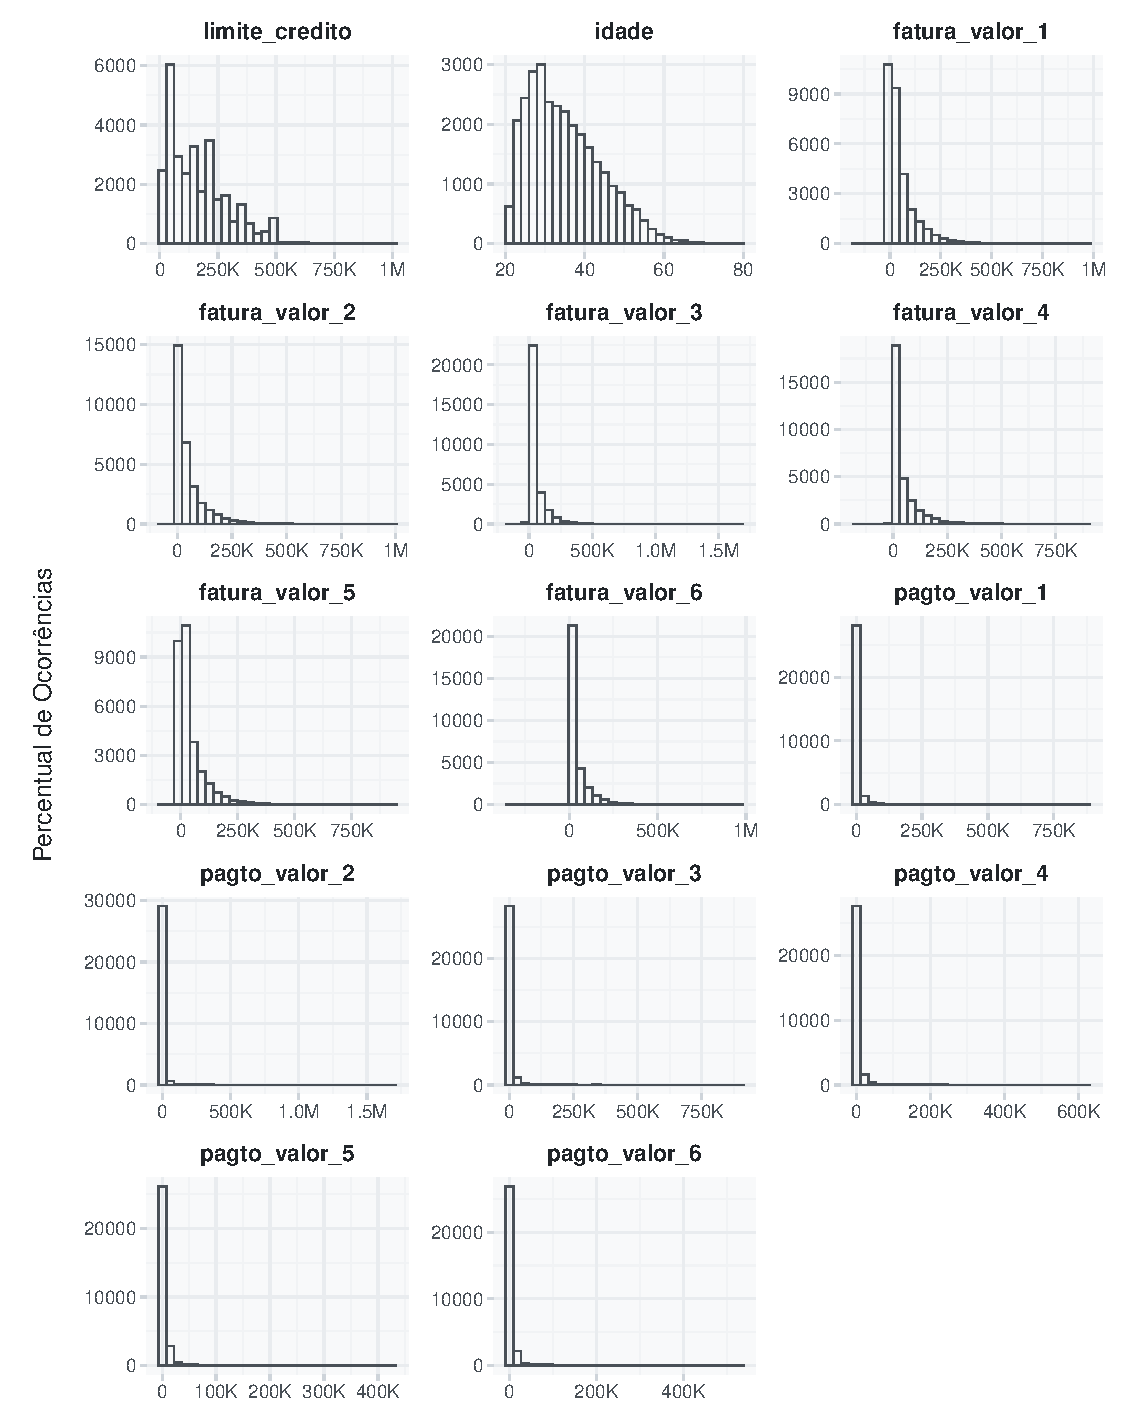
\includegraphics[width=1\linewidth,height=\textheight,keepaspectratio]{monografia_v2_files/figure-pdf/fig-distribuicoes-default-1.pdf}

}

\caption{\label{fig-distribuicoes-default}Distribuição das principais
variáveis numéricas do conjunto de dados}

\end{figure}%

{

\begin{longtable}[]{@{}lrrr@{}}

\caption{\label{tbl-categoricas-default}Distribuição das variáveis
categóricas do conjunto de dados.}

\tabularnewline

\toprule\noalign{}
variavel & categoria & n & percentual (\%) \\
\midrule\noalign{}
\endhead
\bottomrule\noalign{}
\endlastfoot
sexo & 1 & 11888 & 39.63 \\
sexo & 2 & 18112 & 60.37 \\
escolaridade & 0 & 14 & 0.05 \\
escolaridade & 1 & 10585 & 35.28 \\
escolaridade & 2 & 14030 & 46.77 \\
escolaridade & 3 & 4917 & 16.39 \\
escolaridade & 4 & 123 & 0.41 \\
escolaridade & 5 & 280 & 0.93 \\
escolaridade & 6 & 51 & 0.17 \\
estado\_civil & 0 & 54 & 0.18 \\
estado\_civil & 1 & 13659 & 45.53 \\
estado\_civil & 2 & 15964 & 53.21 \\
estado\_civil & 3 & 323 & 1.08 \\

\end{longtable}

}

As variáveis categóricas do conjunto de dados descrevem características
demográficas dos clientes, com distribuições detalhadas na
Tabela~\ref{tbl-categoricas-default}. Observa-se predominância do sexo
feminino e concentração nas categorias ``solteiro'' e ``casado'' para
estado civil. Na escolaridade, predominam os níveis universitário e de
pós-graduação, o que pode estar associado a maior estabilidade de renda
e menores taxas de inadimplência, embora essa relação deva ser avaliada
empiricamente. As subcategorias ``Desconhecido 1'' e ``Desconhecido 2''
foram mantidas como categorias distintas, sem agrupamentos ou
imputações, para preservar a estrutura original da variável.

\subsubsection{Avaliação da variável
resposta}\label{avaliauxe7uxe3o-da-variuxe1vel-resposta}

\begin{figure}

\centering{

\pandocbounded{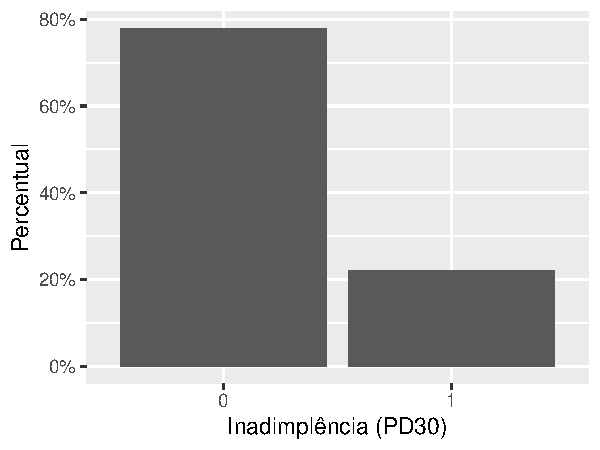
\includegraphics[keepaspectratio]{monografia_v2_files/figure-pdf/fig-target-plot-default-1.pdf}}

}

\caption{\label{fig-target-plot-default}Distribuição da Inadimplência}

\end{figure}%

Na Figura~\ref{fig-target-plot-default}, observa-se a distribuição da
variável resposta PD30, indicando que aproximadamente 22.12\% dos
clientes apresentam inadimplência no mês subsequente, enquanto os demais
77.88\% correspondem à classe de adimplentes. Esse desbalanceamento de
classes é característico de problemas de risco de crédito e deve ser
considerado na etapa de modelagem, uma vez que pode influenciar métricas
de desempenho e a calibração das probabilidades previstas pelos modelos.

Esse cenário é típico de problemas de credit scoring e caracteriza um
contexto de \texttt{imbalanced\ learning}, no qual a classe minoritária
(inadimplência) é justamente a de maior interesse analítico.

Nesse tipo de distribuição, métricas globais como acurácia podem ser
enganosas, pois modelos que privilegiam a classe majoritária tendem a
apresentar desempenho aparentemente elevado mesmo sem capacidade
discriminativa adequada para a classe de interesse. Por essa razão,
métricas baseadas em discriminação e equilíbrio entre classes tornam-se
mais informativas.

\subsubsection{Análise de correlação entre variáveis
numéricas}\label{anuxe1lise-de-correlauxe7uxe3o-entre-variuxe1veis-numuxe9ricas}

\begin{figure}

\centering{

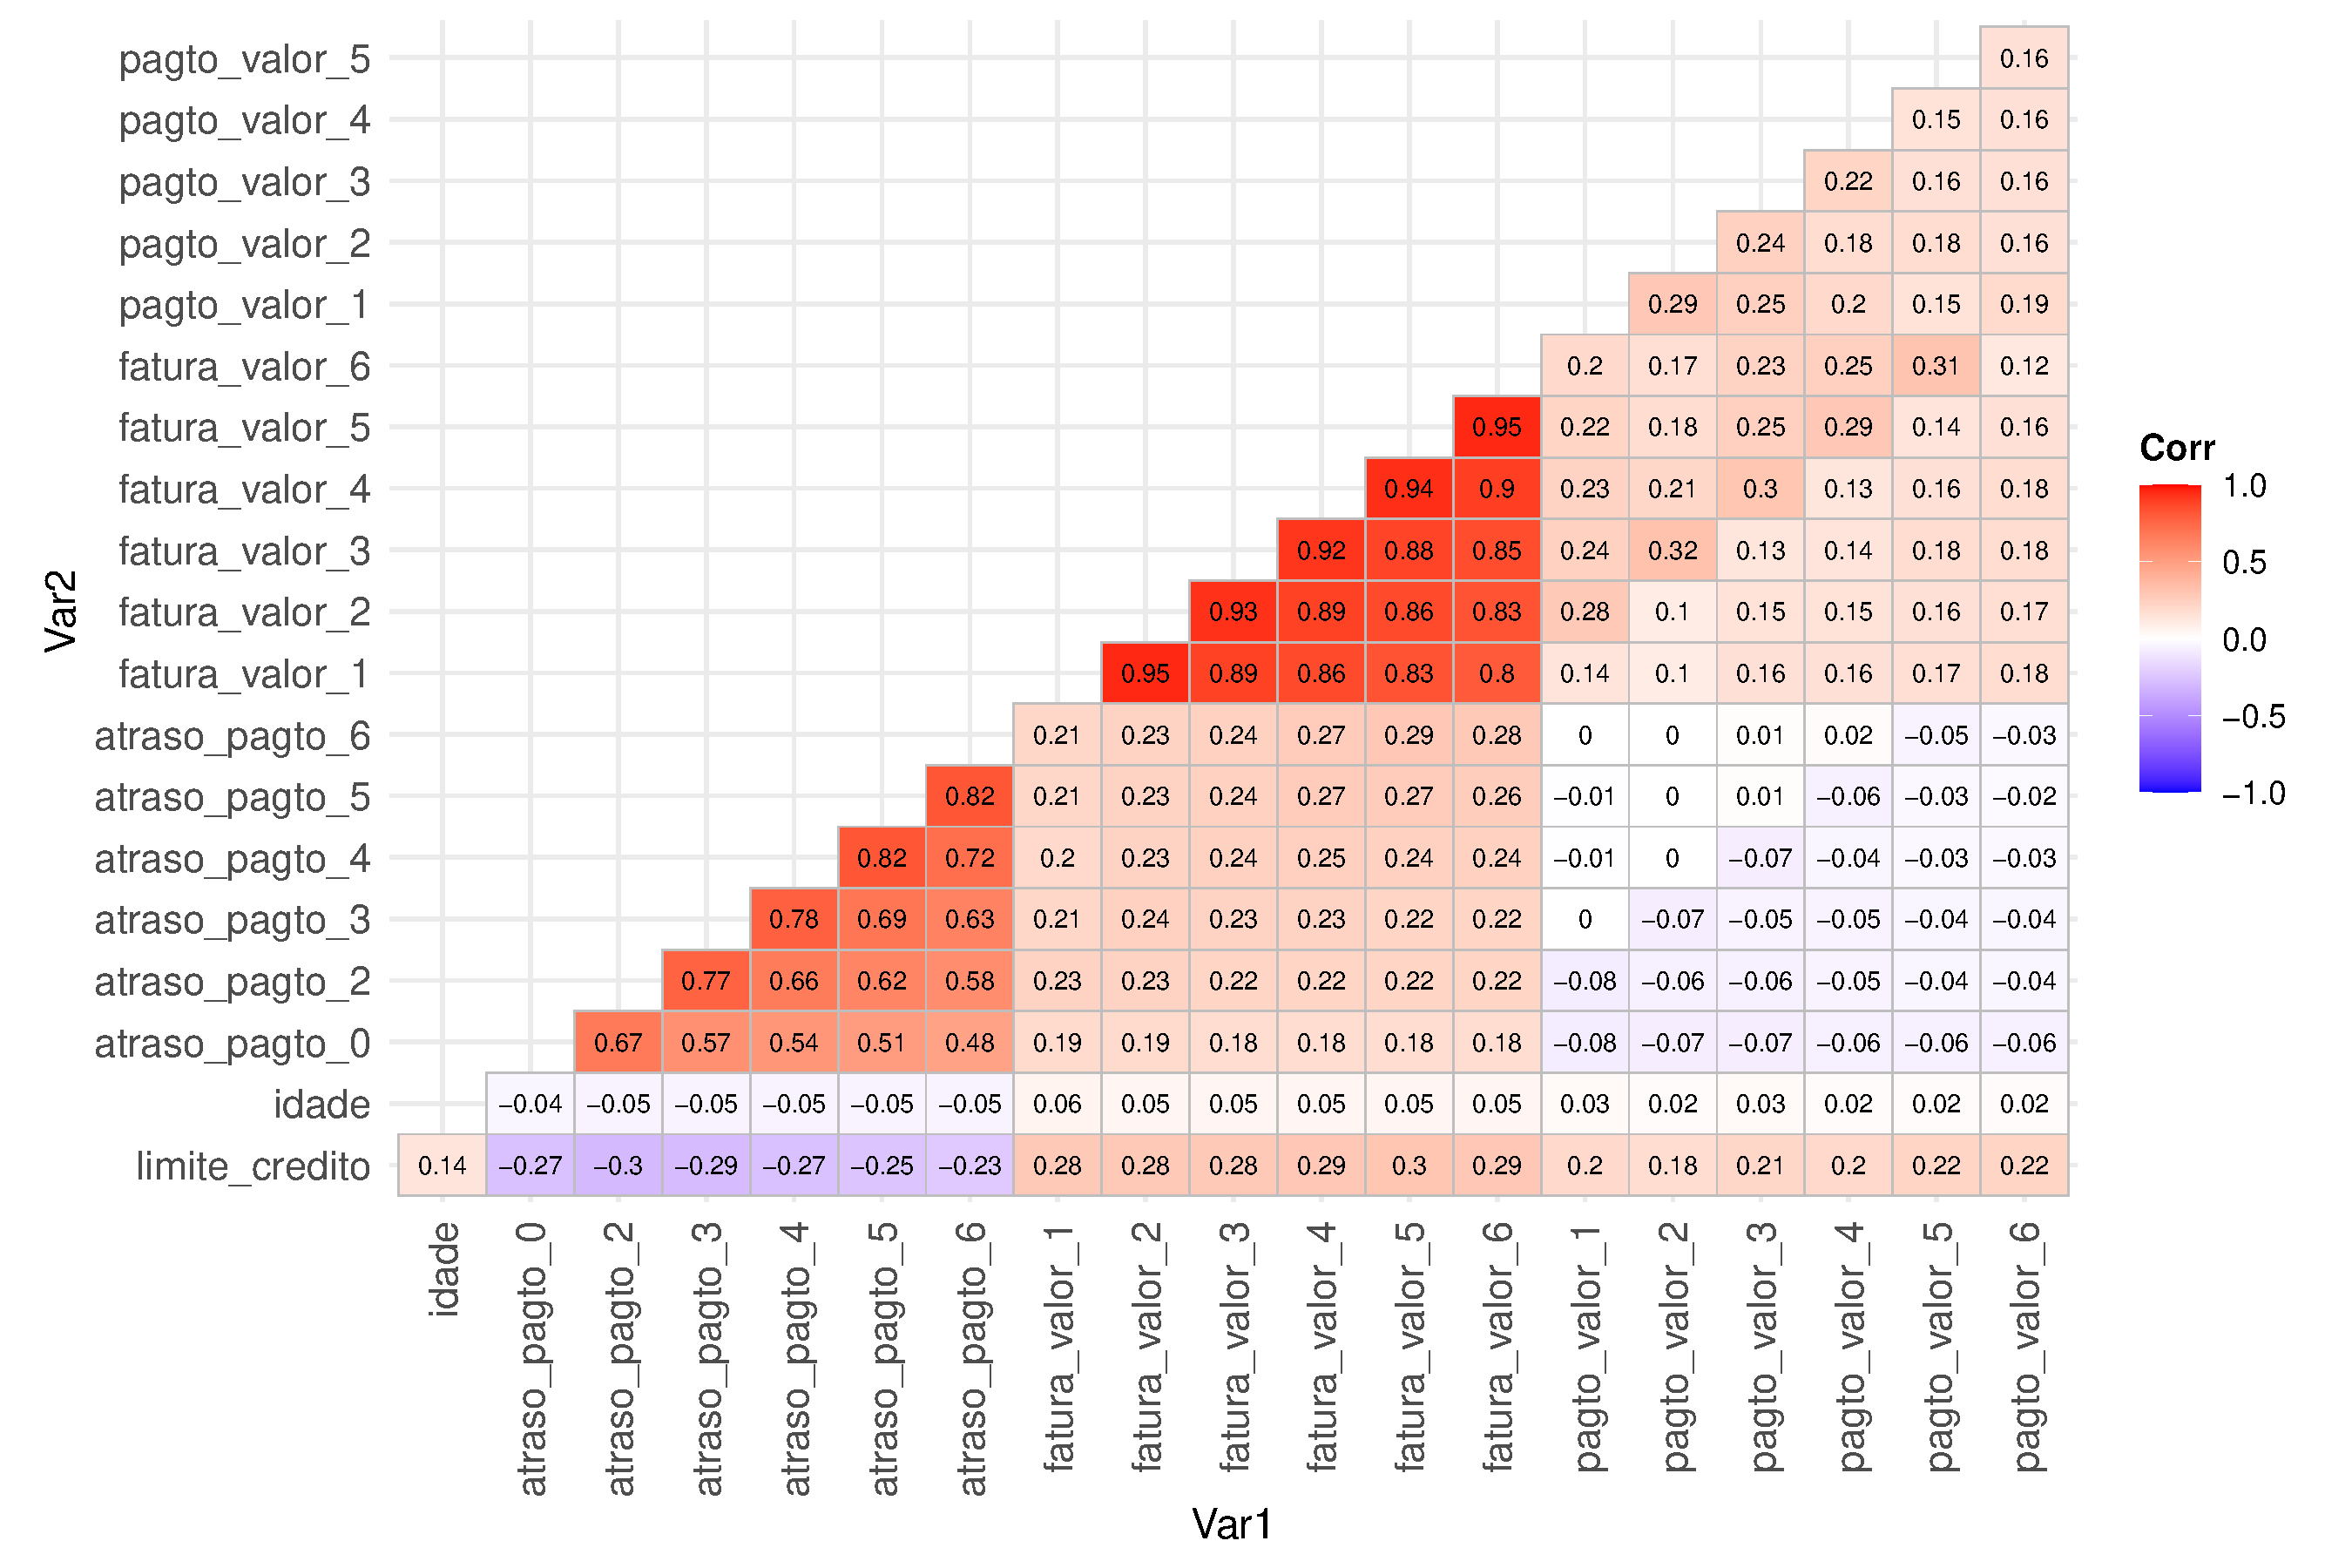
\includegraphics[width=1\linewidth,height=\textheight,keepaspectratio]{monografia_v2_files/figure-pdf/fig-correlacao-default-1.pdf}

}

\caption{\label{fig-correlacao-default}Mapa de calor da correlação entre
variáveis numéricas do conjunto de dados de crédito}

\end{figure}%

A Figura~\ref{fig-correlacao-default} evidencia padrões estruturais
importantes entre as variáveis numéricas do conjunto de dados.
Observa-se uma forte correlação positiva entre os valores de fatura ao
longo dos meses (por exemplo, entre \texttt{fatura\_valor\_1} e
\texttt{fatura\_valor\_2}, com correlação próxima de 0,95), indicando
alta persistência temporal do saldo devedor dos clientes. Esse
comportamento é esperado em dados de crédito, onde o saldo de fatura
tende a evoluir de forma gradual ao longo do tempo.

De forma semelhante, as variáveis de atraso de pagamento
(\texttt{atraso\_pagto\_*}) apresentam correlações moderadas a altas
entre si (chegando a valores acima de 0,8), sugerindo forte dependência
temporal e possível redundância informacional. Esse padrão é relevante
do ponto de vista de modelagem, pois indica potencial multicolinearidade
entre variáveis de comportamento de pagamento, o que pode afetar
estimativas em modelos lineares tradicionais e justificar o uso de
abordagens regularizadas ou bayesianas mais robustas.

Por outro lado, variáveis como idade e limite de crédito apresentam
correlações fracas com a maioria das demais variáveis, sugerindo que
carregam informação relativamente independente dentro do conjunto de
dados. Já os valores de pagamento (\texttt{pagto\_valor\_*}) mostram
correlações baixas entre si e com outras variáveis, indicando maior
variabilidade e menor estrutura temporal consistente quando comparados
aos saldos de fatura e atrasos de pagamento.

\subsubsection{Análise de outliers}\label{anuxe1lise-de-outliers}

{

\begin{longtable}[]{@{}lrr@{}}

\caption{\label{tbl-outliers-default}Número e percentual de outliers
identificados pelo critério do IQR no conjunto de dados de crédito}

\tabularnewline

\toprule\noalign{}
Feature & Outliers & Percentual \\
\midrule\noalign{}
\endhead
\bottomrule\noalign{}
\endlastfoot
atraso\_pagto\_0 & 3130 & 0.1043333 \\
atraso\_pagto\_2 & 4410 & 0.1470000 \\
atraso\_pagto\_3 & 4209 & 0.1403000 \\
atraso\_pagto\_4 & 3508 & 0.1169333 \\
atraso\_pagto\_5 & 2968 & 0.0989333 \\
atraso\_pagto\_6 & 3079 & 0.1026333 \\
fatura\_valor\_1 & 2400 & 0.0800000 \\
fatura\_valor\_2 & 2395 & 0.0798333 \\
fatura\_valor\_3 & 2469 & 0.0823000 \\
fatura\_valor\_4 & 2622 & 0.0874000 \\
fatura\_valor\_5 & 2725 & 0.0908333 \\
fatura\_valor\_6 & 2693 & 0.0897667 \\
idade & 272 & 0.0090667 \\
limite\_credito & 167 & 0.0055667 \\
pagto\_valor\_1 & 2745 & 0.0915000 \\
pagto\_valor\_2 & 2714 & 0.0904667 \\
pagto\_valor\_3 & 2598 & 0.0866000 \\
pagto\_valor\_4 & 2994 & 0.0998000 \\
pagto\_valor\_5 & 2945 & 0.0981667 \\
pagto\_valor\_6 & 2958 & 0.0986000 \\

\end{longtable}

}

Os resultados da detecção de outliers
(Tabela~\ref{tbl-outliers-default}) pelo critério do IQR indicam um
padrão bastante consistente com a natureza dos dados financeiros
analisados. Observa-se que as variáveis relacionadas ao histórico de
atraso de pagamento (\texttt{atraso\_pagto\_*}) apresentam as maiores
proporções de outliers, variando aproximadamente entre 9,9\% e 14,7\%
das observações. Esse comportamento é esperado, uma vez que essas
variáveis são discretas e assimétricas por construção, refletindo
estados de atraso que podem se concentrar em valores extremos (como
atrasos elevados em determinados meses).

As variáveis de valores de fatura (\texttt{fatura\_valor\_*}) e de
pagamento (\texttt{pagto\_valor\_*}) também apresentam proporções
relevantes de outliers, em torno de 8\% a 9\%. Isso é típico em dados
financeiros de crédito, nos quais distribuições são fortemente
assimétricas à direita, com uma pequena parcela de clientes concentrando
valores elevados de consumo e pagamento. Nesse contexto, esses
``outliers'' não necessariamente representam erros ou anomalias, mas sim
a própria heterogeneidade do comportamento financeiro da população.

Em contraste, variáveis como idade e limite de crédito apresentam
proporções muito baixas de outliers (inferiores a 1\%), sugerindo
distribuições mais estáveis e próximas de um comportamento
aproximadamente simétrico ou moderadamente disperso. Esse resultado
reforça a importância de interpretar outliers sob uma perspectiva
contextual: em dados de crédito, valores extremos frequentemente
carregam informação relevante sobre risco e capacidade financeira, não
devendo ser removidos automaticamente sem análise substantiva.

\subsection{Pré processamento do
dataset}\label{pruxe9-processamento-do-dataset}

Inicialmente, foi realizada a verificação da presença de valores
ausentes e observações duplicadas no conjunto de dados analisado. Não
foram identificados valores faltantes ou registros duplicados, o que
dispensou a aplicação de técnicas de imputação e garantiu a consistência
estrutural das bases utilizadas.

Em relação aos outliers, optou-se por não aplicar procedimentos de
remoção ou transformação em ambos os conjuntos de dados. A identificação
pelo critério do intervalo interquartil (IQR) revelou a presença de
valores extremos em variáveis financeiras e comportamentais, o que é
esperado em bases de crédito devido à forte assimetria e heterogeneidade
dos perfis de clientes. Nesses contextos, valores extremos não são
necessariamente indicativos de erro, podendo representar justamente os
casos de maior interesse analítico, especialmente em tarefas de
modelagem de risco de crédito.

\subsubsection{Seleção de variáveis e análise de
correlação}\label{seleuxe7uxe3o-de-variuxe1veis-e-anuxe1lise-de-correlauxe7uxe3o}

A Figura~\ref{fig-correlacao-default} foi utilizada para investigar
possíveis relações de dependência linear entre as variáveis numéricas
dos dois conjuntos de dados analisados. Em ambos os casos, observam-se
padrões consistentes de correlação estrutural entre variáveis
financeiras, especialmente aquelas relacionadas a renda, patrimônio e
exposição de crédito.

Apesar da presença de relações entre variáveis financeiras e
comportamentais, optou-se por não realizar remoção de variáveis nesta
etapa. Essa decisão foi orientada pelo objetivo de manter
comparabilidade entre abordagens de modelagem e preservar o espaço
completo de informação para avaliação empírica posterior.

Adicionalmente, a eventual presença de redundância informacional será
tratada implicitamente pelos próprios modelos considerados, incluindo
regressão logística regularizada e abordagens bayesianas, além de ser
avaliada posteriormente por métricas complementares como o Variance
Inflation Factor (VIF). Isso permite uma análise mais controlada do
impacto da estrutura de dependência entre variáveis sobre desempenho
preditivo e interpretabilidade.

\subsubsection{Separação
treino/teste}\label{separauxe7uxe3o-treinoteste}

Os conjuntos de dados foram divididos aleatoriamente em subconjuntos de
treino (75\%) e teste (25\%), utilizando amostragem estratificada em
relação às variáveis resposta. Essa estratégia assegura que a proporção
de observações pertencentes a cada classe seja preservada em ambos os
subconjuntos.

O ajuste do modelo foi realizado exclusivamente com o conjunto de
treino, enquanto o conjunto de teste foi reservado para a avaliação do
desempenho preditivo fora da amostra, assegurando a separação adequada
entre as etapas de estimação e validação.

\subsection{Modelagem e Avaliação}\label{modelagem-e-avaliauxe7uxe3o}

Após a etapa de pré-processamento, o conjunto de dados de concessão de
empréstimos foi utilizado para o ajuste de modelos de regressão
logística, com o objetivo de estimar a probabilidade de default (PD30) a
partir das características socioeconômicas e financeiras dos clientes. A
regressão logística foi escolhida por se tratar de um modelo amplamente
utilizado em problemas de classificação binária e por permitir a
interpretação dos efeitos das variáveis explicativas sobre as chances do
evento de interesse por meio das razões de chances (odds ratios). A
partir dessa mesma estrutura de modelagem, foram consideradas as
abordagens frequentista e Bayesiana, permitindo comparar não apenas o
desempenho preditivo, mas também as diferentes formas de estimação e
inferência sobre os parâmetros do modelo.

\subsubsection{Modelagem Frequentista}\label{modelagem-frequentista}

Inicialmente, adotou-se uma abordagem frequentista, com estimação dos
parâmetros via máxima verossimilhança. Essa estratégia fornece um ponto
de partida robusto para a análise, permitindo avaliar tanto o poder
preditivo quanto a contribuição individual das variáveis explicativas.

Com o intuito de investigar a sensibilidade do modelo à especificação
das variáveis e à presença de dependências lineares, foram ajustadas
diferentes variações do modelo logístico:

\begin{itemize}
\item
  \textbf{Modelo completo:} inclui todas as variáveis explicativas
  disponíveis após o pré-processamento, servindo como especificação de
  referência para as comparações.
\item
  \textbf{Modelo com remoção manual de variáveis altamente
  correlacionadas:} variáveis com correlação absoluta superior a 75\%
  foram excluídas de forma criteriosa, visando reduzir a redundância
  informacional e avaliar o impacto dessa simplificação na estabilidade
  e no desempenho do modelo.
\item
  \textbf{Modelo com regularização L1 (Lasso):} incorpora uma
  penalização baseada na soma dos valores absolutos dos coeficientes,
  favorecendo a redução de sua magnitude e podendo levar alguns deles a
  valores exatamente iguais a zero. Dessa forma, além de controlar a
  complexidade do modelo, essa abordagem pode promover uma seleção
  implícita de variáveis.
\item
  \textbf{Modelo com regularização L2 (Ridge):} utiliza uma penalização
  baseada na soma dos quadrados dos coeficientes, promovendo sua redução
  em direção a zero, mas sem anulá-los. Seu objetivo é controlar a
  magnitude dos parâmetros e reduzir a sensibilidade do modelo a
  variáveis explicativas correlacionadas.
\end{itemize}

Quanto ao pré-processamento, a padronização das variáveis numéricas foi
aplicada aos modelos com regularização L1 e L2, uma vez que a
penalização depende da magnitude dos coeficientes e, portanto, é
sensível à escala das variáveis. Nos modelos sem regularização, a
padronização não foi aplicada, preservando-se as escalas originais para
facilitar a interpretação dos coeficientes.

A comparação entre essas especificações permite avaliar o trade-off
entre interpretabilidade, complexidade do modelo e desempenho preditivo,
além de fornecer evidências empíricas sobre o papel do score de crédito
e da estrutura de correlação das variáveis no processo de decisão de
concessão de empréstimos.

Após o pré-processamento, diferentes especificações de modelos de
regressão logística foram ajustadas com base em máxima verossimilhança.
Todas as especificações propostas foram avaliadas de forma sistemática
quanto ao ajuste estatístico e às propriedades inferenciais do modelo,
incluindo interpretação dos coeficientes, razões de chances (odds
ratios), testes de razão de verossimilhança, critérios de informação
(AIC e BIC), diagnóstico de multicolinearidade (VIF) e análise de
resíduos.

{

\begin{longtable}[]{@{}
  >{\raggedright\arraybackslash}p{(\linewidth - 10\tabcolsep) * \real{0.2255}}
  >{\raggedleft\arraybackslash}p{(\linewidth - 10\tabcolsep) * \real{0.1373}}
  >{\raggedleft\arraybackslash}p{(\linewidth - 10\tabcolsep) * \real{0.1765}}
  >{\raggedleft\arraybackslash}p{(\linewidth - 10\tabcolsep) * \real{0.0882}}
  >{\raggedleft\arraybackslash}p{(\linewidth - 10\tabcolsep) * \real{0.0882}}
  >{\raggedleft\arraybackslash}p{(\linewidth - 10\tabcolsep) * \real{0.2843}}@{}}

\caption{\label{tbl-diagnosticos-glm-pd30}Estatísticas de ajuste dos
modelos de regressão logística não penalizados}

\tabularnewline

\toprule\noalign{}
\begin{minipage}[b]{\linewidth}\raggedright
Modelo
\end{minipage} & \begin{minipage}[b]{\linewidth}\raggedleft
Deviance nula
\end{minipage} & \begin{minipage}[b]{\linewidth}\raggedleft
Deviance residual
\end{minipage} & \begin{minipage}[b]{\linewidth}\raggedleft
AIC
\end{minipage} & \begin{minipage}[b]{\linewidth}\raggedleft
BIC
\end{minipage} & \begin{minipage}[b]{\linewidth}\raggedleft
Graus de liberdade residuais
\end{minipage} \\
\midrule\noalign{}
\endhead
\bottomrule\noalign{}
\endlastfoot
Completo & 23779.02 & 20797.50 & 20855.50 & 21088.11 & 22471 \\
Sem multicolinearidade & 23779.02 & 20848.41 & 20890.41 & 21058.85 &
22479 \\

\end{longtable}

}

A comparação das estatísticas de ajuste foi realizada apenas para os
modelos de regressão logística não penalizados (Completo e Sem
multicolinearidade), uma vez que ambos foram estimados pelo método
tradicional de máxima verossimilhança, permitindo a obtenção e a
interpretação direta de medidas como a deviance residual, o AIC e o BIC.
Os modelos Lasso (L1) e Ridge (L2), por sua vez, incorporam penalizações
sobre os coeficientes e são estimados por meio do pacote glmnet, de modo
que os critérios tradicionais de informação não são diretamente
equivalentes aos calculados para os modelos não penalizados. Por essa
razão, a comparação desses modelos foi conduzida principalmente com base
nas métricas de desempenho preditivo.

Conforme apresentado na Tabela~\ref{tbl-diagnosticos-glm-pd30}, o modelo
Completo apresentou menor deviance residual em relação ao modelo Sem
multicolinearidade, além de menores valores de AIC. Esses resultados
indicam um melhor ajuste do modelo completo segundo essas medidas. Em
contrapartida, o modelo Sem multicolinearidade apresentou menor BIC,
favorecendo a especificação mais parcimoniosa, que também possui oito
graus de liberdade residuais adicionais, correspondentes a uma estrutura
com oito parâmetros a menos.

De modo geral, os resultados apontam para um equilíbrio entre qualidade
de ajuste e parcimônia: enquanto o modelo Completo é favorecido pela
deviance residual e pelo AIC, o modelo Sem multicolinearidade apresenta
vantagem segundo o BIC. Essas diferenças são consideradas em conjunto
com os resultados das métricas preditivas, apresentados a seguir.

{

\begin{longtable}[]{@{}
  >{\raggedright\arraybackslash}p{(\linewidth - 8\tabcolsep) * \real{0.2703}}
  >{\raggedleft\arraybackslash}p{(\linewidth - 8\tabcolsep) * \real{0.1216}}
  >{\raggedleft\arraybackslash}p{(\linewidth - 8\tabcolsep) * \real{0.3108}}
  >{\raggedleft\arraybackslash}p{(\linewidth - 8\tabcolsep) * \real{0.1486}}
  >{\raggedleft\arraybackslash}p{(\linewidth - 8\tabcolsep) * \real{0.1486}}@{}}

\caption{\label{tbl-metricas-modelos-pd30}Métricas de desempenho do
modelo de regressão logística, avaliadas no conjunto de teste.}

\tabularnewline

\toprule\noalign{}
\begin{minipage}[b]{\linewidth}\raggedright
Métrica
\end{minipage} & \begin{minipage}[b]{\linewidth}\raggedleft
Completo
\end{minipage} & \begin{minipage}[b]{\linewidth}\raggedleft
Sem multicolinearidade
\end{minipage} & \begin{minipage}[b]{\linewidth}\raggedleft
Lasso (L1)
\end{minipage} & \begin{minipage}[b]{\linewidth}\raggedleft
Ridge (L2)
\end{minipage} \\
\midrule\noalign{}
\endhead
\bottomrule\noalign{}
\endlastfoot
Acurácia & 0.811 & 0.812 & 0.811 & 0.807 \\
Acurácia balanceada & 0.613 & 0.613 & 0.613 & 0.599 \\
ROC-AUC & 0.716 & 0.714 & 0.716 & 0.715 \\
Log-loss & 0.470 & 0.470 & 0.470 & 0.469 \\
Sensibilidade & 0.259 & 0.258 & 0.258 & 0.226 \\
Especificidade & 0.967 & 0.969 & 0.968 & 0.972 \\
Precisão & 0.692 & 0.703 & 0.695 & 0.696 \\
F1-score & 0.376 & 0.377 & 0.376 & 0.341 \\
MCC & 0.340 & 0.345 & 0.341 & 0.318 \\

\end{longtable}

}

{

\begin{longtable}[]{@{}lcc@{}}

\caption{\label{tbl-vif-modelos-pd30}Resumo do VIF para os modelos de
regressão logística não penalizados.}

\tabularnewline

\toprule\noalign{}
Modelo & VIF máximo & VIF médio \\
\midrule\noalign{}
\endhead
\bottomrule\noalign{}
\endlastfoot
Completo & 41.12 & 7.80 \\
Sem multicolinearidade & 1.84 & 1.24 \\

\end{longtable}

}

As quatro especificações apresentaram desempenho preditivo bastante
semelhante (Tabela~\ref{tbl-metricas-modelos-pd30}): ROC AUC entre 0,714
e 0,716, log-loss em torno de 0,47 e acurácia entre 0,807 e 0,812. O
modelo L2 (Ridge) é a única exceção parcial: apresentou a menor
sensibilidade (0,226) e a maior especificidade (0,972), em contraste com
os demais modelos, que mantiveram acurácia balanceada próxima de 0,613.
As diferenças observadas são pequenas, indicando que a remoção de
variáveis correlacionadas ou a aplicação das penalizações não produziu
alterações substanciais na capacidade discriminativa.

A análise do VIF (Tabela~\ref{tbl-vif-modelos-pd30}) evidencia uma
diferença mais pronunciada entre as especificações: o modelo completo
apresentou VIF máximo de 41,12 e médio de 7,80, enquanto o modelo sem
multicolinearidade reduziu esses valores para 1,84 e 1,24,
respectivamente --- redução substancial sem alteração relevante no
desempenho preditivo. Os modelos regularizados L1 e L2 não são avaliados
por VIF porque a regularização atua sobre os coeficientes durante a
estimação, não sobre a estrutura de correlação dos preditores; assim,
são comparados principalmente com base no desempenho preditivo e no
comportamento dos coeficientes.

Um aspecto comum às quatro especificações é a elevada especificidade
(entre 0,967 e 0,972) acompanhada por baixa sensibilidade (entre 0,226 e
0,259). Esse comportamento indica que os modelos identificam
corretamente a grande maioria dos não inadimplentes, mas classificam
incorretamente parcela expressiva dos inadimplentes, resultado
consistente com o desbalanceamento da variável resposta e que deve ser
considerado na interpretação da acurácia global.

\paragraph{Comparações de Features L1 vs Remoção de Variáveis
Correlacionadas}\label{comparauxe7uxf5es-de-features-l1-vs-remouxe7uxe3o-de-variuxe1veis-correlacionadas}

A comparação entre as estratégias de redução da complexidade revelou uma
sobreposição parcial entre as variáveis excluídas pelo procedimento de
correlação e aquelas cujos coeficientes foram anulados pela
regularização L1. Em particular, a variável \texttt{fatura\_valor\_4}
foi removida em ambas as abordagens. Entretanto, o L1 também anulou o
coeficiente de \texttt{fatura\_valor\_6}, enquanto o procedimento
baseado em correlação excluiu outras variáveis, como
\texttt{atraso\_pagto\_3}, \texttt{atraso\_pagto\_4},
\texttt{atraso\_pagto\_5} e \texttt{fatura\_valor\_5}.

Essa sobreposição limitada indica que as estratégias não são
equivalentes: enquanto a remoção por correlação considera a associação
entre os preditores, a penalização L1 seleciona variáveis com base na
contribuição conjunta para o ajuste do modelo, condicionada à
penalização aplicada. Assim, embora ambas possam reduzir a complexidade
da especificação, seus critérios de seleção produzem conjuntos distintos
de variáveis.

\paragraph{Seleção da especificação para a análise
inferencial}\label{seleuxe7uxe3o-da-especificauxe7uxe3o-para-a-anuxe1lise-inferencial}

A análise inferencial detalhada será concentrada no modelo sem
multicolinearidade. Essa escolha não decorre de superioridade preditiva,
uma vez que os quatro modelos apresentaram métricas bastante próximas,
mas da combinação entre a redução substancial do VIF (de 41,12 para
1,84) e a manutenção da estrutura convencional da regressão logística
estimada por MLE, que viabiliza o uso direto de erros-padrão, intervalos
de confiança, testes de significância e razões de chances. A menor
multicolinearidade também reduz a instabilidade das estimativas e
facilita a interpretação individual dos coeficientes, condição relevante
para a comparação com a abordagem bayesiana.

Os modelos L1 e L2 permanecem como referências na avaliação do
desempenho preditivo. Entretanto, a estimação penalizada não fornece
erros-padrão convencionais de forma direta, inviabilizando os
procedimentos inferenciais usuais; além disso, a penalização L1 pode
anular coeficientes, incorporando seleção de variáveis à estimação. Por
essas razões, a análise de diagnóstico e interpretação detalhada será
conduzida com base no modelo sem multicolinearidade, que preserva a
estrutura completa da regressão logística tradicional.

\paragraph{Diagnóstico do modelo modelo sem
multicolinearidade}\label{diagnuxf3stico-do-modelo-modelo-sem-multicolinearidade}

\begin{figure}

\centering{

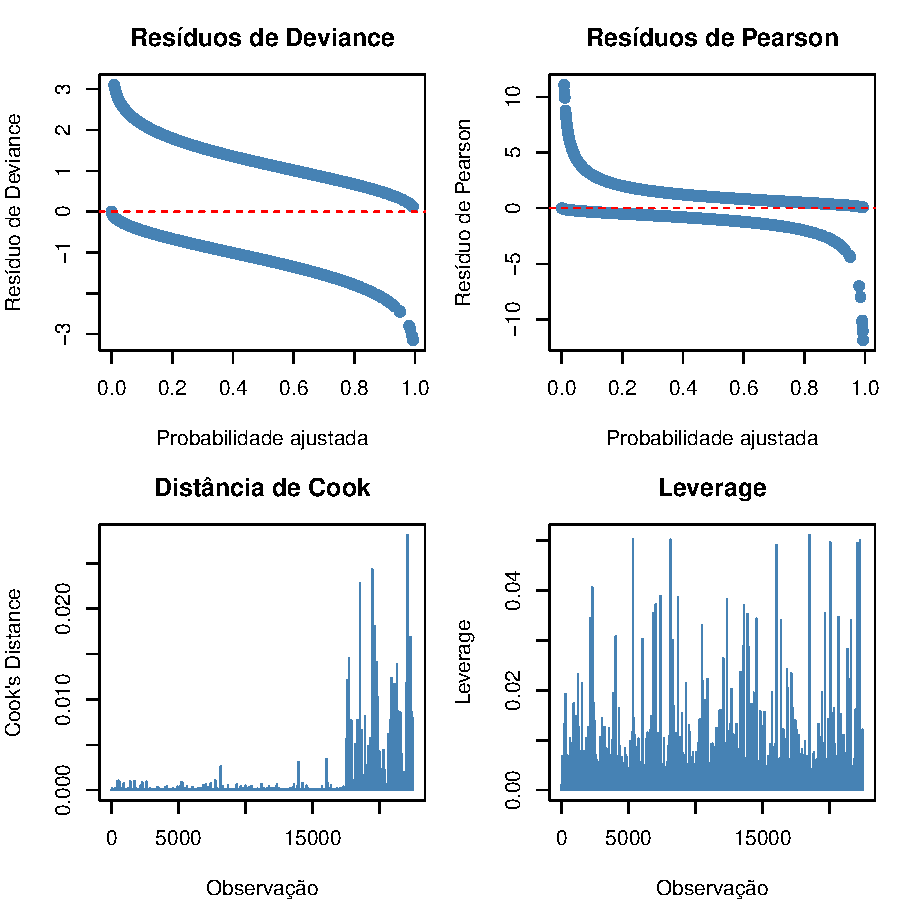
\includegraphics[width=0.75\linewidth,height=\textheight,keepaspectratio]{monografia_v2_files/figure-pdf/fig-default-residuos-1.pdf}

}

\caption{\label{fig-default-residuos}Análise de resíduos do modelo de
regressão logística sem multicolinearidade.}

\end{figure}%

A adequação do ajuste foi investigada por meio dos resíduos de Deviance
e de Pearson, da distância de Cook e do \emph{leverage}, conforme
apresentado na Figura~\ref{fig-default-residuos}. Os gráficos de
resíduos apresentam a formação de dois ramos, comportamento esperado em
modelos logísticos com resposta binária. Os resíduos de Pearson mostram
algumas observações de maior magnitude nas regiões de probabilidades
extremas, compatíveis com a natureza probabilística do modelo.

A distância de Cook apresenta valores próximos de zero para a maior
parte das observações, com máximo em torno de 0,028; o \emph{leverage}
atinge aproximadamente 0,05 nas observações de maior alavancagem. De
modo geral, os diagnósticos não evidenciam padrão generalizado de
influência ou inadequação estrutural que comprometa a utilização do
modelo.

{

\begin{longtable}[]{@{}lrrl@{}}

\caption{\label{tbl-drop1-pd30}Teste da razão de verossimilhanças para a
contribuição individual dos termos do modelo.}

\tabularnewline

\toprule\noalign{}
Variável & Graus de liberdade & Deviance & p-valor \\
\midrule\noalign{}
\endhead
\bottomrule\noalign{}
\endlastfoot
limite\_credito & 1 & 16.473 & \textless{} 0.001 \\
idade & 1 & 7.248 & 0.0071 \\
atraso\_pagto\_0 & 1 & 864.352 & \textless{} 0.001 \\
atraso\_pagto\_2 & 1 & 48.532 & \textless{} 0.001 \\
atraso\_pagto\_6 & 1 & 19.514 & \textless{} 0.001 \\
fatura\_valor\_1 & 1 & 33.057 & \textless{} 0.001 \\
pagto\_valor\_1 & 1 & 18.374 & \textless{} 0.001 \\
pagto\_valor\_2 & 1 & 20.785 & \textless{} 0.001 \\
pagto\_valor\_3 & 1 & 1.905 & 0.1675 \\
pagto\_valor\_4 & 1 & 10.725 & 0.0011 \\
pagto\_valor\_5 & 1 & 6.159 & 0.0131 \\
pagto\_valor\_6 & 1 & 4.122 & 0.0423 \\
sexo\_Feminino & 1 & 15.050 & \textless{} 0.001 \\
escolaridade\_Universidade & 1 & 3.139 & 0.0764 \\
escolaridade\_EnsinoMedio & 1 & 4.829 & 0.0280 \\
escolaridade\_Outros & 1 & 6.868 & 0.0088 \\
escolaridade\_Desconhecido1 & 1 & 47.049 & \textless{} 0.001 \\
escolaridade\_Desconhecido2 & 1 & 0.006 & 0.9392 \\
estado\_civil\_Solteiro & 1 & 19.567 & \textless{} 0.001 \\
estado\_civil\_Outros & 1 & 0.528 & 0.4674 \\

\end{longtable}

}

A contribuição individual dos termos do modelo foi avaliada por meio do
teste da razão de verossimilhanças (Tabela~\ref{tbl-drop1-pd30}), que
compara o modelo completo com versões nas quais cada preditor é removido
individualmente. \texttt{atraso\_pagto\_0} apresenta a maior
contribuição, com redução de 864 unidades na Deviance (p \textless{}
0,001), seguido de \texttt{atraso\_pagto\_2},
\texttt{escolaridade\_Desconhecido1}, \texttt{fatura\_valor\_1} e demais
variáveis de comportamento de pagamento e demográficas, com p
\textless{} 0,001 ou p \textless{} 0,05. Quatro termos não atingiram
significância ao nível de 5\%: \texttt{pagto\_valor\_3},
\texttt{escolaridade\_Universidade},
\texttt{escolaridade\_Desconhecido2} e \texttt{estado\_civil\_Outros}.

Cabe observar que a ausência de significância individual não implica
irrelevância para o modelo: o teste avalia a contribuição de cada termo
condicionada à presença dos demais, e a significância estatística não
corresponde, por si só, à magnitude do efeito prático.

{

\begin{longtable}[]{@{}
  >{\raggedright\arraybackslash}p{(\linewidth - 10\tabcolsep) * \real{0.3913}}
  >{\raggedleft\arraybackslash}p{(\linewidth - 10\tabcolsep) * \real{0.1304}}
  >{\raggedleft\arraybackslash}p{(\linewidth - 10\tabcolsep) * \real{0.1449}}
  >{\raggedleft\arraybackslash}p{(\linewidth - 10\tabcolsep) * \real{0.1449}}
  >{\raggedleft\arraybackslash}p{(\linewidth - 10\tabcolsep) * \real{0.1159}}
  >{\raggedleft\arraybackslash}p{(\linewidth - 10\tabcolsep) * \real{0.0725}}@{}}

\caption{\label{tbl-complete-model-default}Resultados da estimação do
modelo de regressão logística frequentista}

\tabularnewline

\toprule\noalign{}
\begin{minipage}[b]{\linewidth}\raggedright
term
\end{minipage} & \begin{minipage}[b]{\linewidth}\raggedleft
estimate
\end{minipage} & \begin{minipage}[b]{\linewidth}\raggedleft
std.error
\end{minipage} & \begin{minipage}[b]{\linewidth}\raggedleft
statistic
\end{minipage} & \begin{minipage}[b]{\linewidth}\raggedleft
p.value
\end{minipage} & \begin{minipage}[b]{\linewidth}\raggedleft
OR
\end{minipage} \\
\midrule\noalign{}
\endhead
\bottomrule\noalign{}
\endlastfoot
(Intercept) & -0.99 & 0.10 & -9.93 & 0.00 & 0.37 \\
limite\_credito & 0.00 & 0.00 & -4.03 & 0.00 & 1.00 \\
idade & 0.01 & 0.00 & 2.70 & 0.01 & 1.01 \\
atraso\_pagto\_0 & 0.60 & 0.02 & 29.41 & 0.00 & 1.82 \\
atraso\_pagto\_2 & 0.13 & 0.02 & 6.99 & 0.00 & 1.14 \\
atraso\_pagto\_6 & 0.08 & 0.02 & 4.41 & 0.00 & 1.08 \\
fatura\_valor\_1 & 0.00 & 0.00 & -5.67 & 0.00 & 1.00 \\
pagto\_valor\_1 & 0.00 & 0.00 & -3.74 & 0.00 & 1.00 \\
pagto\_valor\_2 & 0.00 & 0.00 & -3.93 & 0.00 & 1.00 \\
pagto\_valor\_3 & 0.00 & 0.00 & -1.32 & 0.19 & 1.00 \\
pagto\_valor\_4 & 0.00 & 0.00 & -2.97 & 0.00 & 1.00 \\
pagto\_valor\_5 & 0.00 & 0.00 & -2.31 & 0.02 & 1.00 \\
pagto\_valor\_6 & 0.00 & 0.00 & -1.94 & 0.05 & 1.00 \\
sexo\_Feminino & -0.14 & 0.04 & -3.89 & 0.00 & 0.87 \\
escolaridade\_Universidade & -0.07 & 0.04 & -1.77 & 0.08 & 0.93 \\
escolaridade\_EnsinoMedio & -0.12 & 0.06 & -2.19 & 0.03 & 0.89 \\
escolaridade\_Outros & -0.99 & 0.43 & -2.29 & 0.02 & 0.37 \\
escolaridade\_Desconhecido1 & -1.86 & 0.35 & -5.25 & 0.00 & 0.15 \\
escolaridade\_Desconhecido2 & 0.03 & 0.45 & 0.08 & 0.94 & 1.03 \\
estado\_civil\_Solteiro & -0.18 & 0.04 & -4.42 & 0.00 & 0.84 \\
estado\_civil\_Outros & -0.12 & 0.16 & -0.72 & 0.47 & 0.89 \\

\end{longtable}

}

A Tabela~\ref{tbl-complete-model-default} apresenta os coeficientes
estimados, erros-padrão, estatísticas de teste, p-valores e razões de
chances (OR). Entre os preditores avaliados, \texttt{atraso\_pagto\_0}
destaca-se como a variável de maior impacto positivo, com coeficiente de
0,5984 e OR de 1,82 --- mantidos os demais preditores constantes, sua
presença está associada a aproximadamente 1,82 vezes as chances de PD30.
As variáveis \texttt{atraso\_pagto\_2} e \texttt{atraso\_pagto\_6}
também apresentam associações positivas, embora de menor magnitude.
Entre os efeitos negativos, \texttt{sexo\_Feminino} (OR = 0,87; p
\textless{} 0,001) e \texttt{estado\_civil\_Solteiro} (OR = 0,84; p
\textless{} 0,001) estão associados a menores chances de inadimplência.
A categoria \texttt{escolaridade\_Desconhecido1} apresenta o maior
efeito negativo (OR = 0,15; p \textless{} 0,001), embora deva ser
interpretada com cautela, pois pode representar ausência de informação
no processo de coleta, não um nível substantivo de escolaridade.

Os termos relacionados a valores de fatura, pagamento e limite de
crédito apresentam coeficientes numericamente pequenos pelo fato de
essas variáveis serem medidas em escala monetária, na qual uma unidade
representa variação relativamente pequena. Os coeficientes arredondados
a quatro casas decimais aparecem como 0,0000 e ORs como 1,0000, sem que
isso implique ausência de efeito --- a interpretação adequada considera
variações economicamente relevantes na escala original. Nesse grupo,
\texttt{fatura\_valor\_1}, \texttt{pagto\_valor\_1},
\texttt{pagto\_valor\_2}, \texttt{pagto\_valor\_4} e
\texttt{pagto\_valor\_5} apresentam associação estatisticamente
significativa com PD30.

Em conjunto, os coeficientes evidenciam associações de diferentes
magnitudes e direções, com destaque para os preditores de comportamento
de pagamento. A análise das ORs complementa o teste da razão de
verossimilhanças apresentado anteriormente, permitindo caracterizar
tanto a direção dos efeitos quanto sua relevância individual no modelo.

\subsubsection{Modelagem Bayesiana}\label{modelagem-bayesiana}

Para avaliar a influência da especificação da distribuição a priori
sobre as estimativas posteriores, foram consideradas duas distribuições
distintas: Normal e Laplace, ambas centradas em zero e com escala igual
a um. A distribuição Normal estabelece uma contração contínua e
simétrica dos coeficientes, enquanto a distribuição Laplace apresenta
maior concentração em torno de zero e caudas mais pesadas, permitindo
investigar uma estratégia alternativa de regularização. Em ambos os
modelos, foi utilizada uma distribuição Normal com média zero e
desvio-padrão cinco para o intercepto, permitindo maior flexibilidade na
estimação desse parâmetro.

\paragraph{Diagnóstico de
multicolinearidade}\label{diagnuxf3stico-de-multicolinearidade-1}

{

\begin{longtable}[]{@{}rr@{}}

\caption{\label{tbl-vif-bayes}Valores máximo e médio dos fatores de
inflação da variância (VIF) dos modelos bayesianos.}

\tabularnewline

\toprule\noalign{}
VIF máximo & VIF médio \\
\midrule\noalign{}
\endhead
\bottomrule\noalign{}
\endlastfoot
25.88 & 6.08 \\

\end{longtable}

}

O diagnóstico de multicolinearidade foi realizado a partir dos fatores
de inflação da variância (\emph{Variance Inflation Factor}, VIF) dos
preditores utilizados nas especificações bayesianas. Como os modelos com
priors Normal e Laplace compartilham a mesma matriz de preditores, os
valores de VIF são idênticos para ambas as especificações, sendo
apresentados conjuntamente na Tabela~\ref{tbl-vif-bayes}.

Os resultados revelaram que a multicolinearidade está concentrada
principalmente nas variáveis referentes aos valores das faturas mensais
(\texttt{fatura\_valor\_1} a \texttt{fatura\_valor\_6}), cujos VIFs
variaram entre 14,35 e 25,88. As variáveis relacionadas ao histórico de
atrasos (\texttt{atraso\_pagto}) apresentaram valores intermediários,
entre 1,89 e 4,70, enquanto os demais preditores registraram VIFs
inferiores a 2.

Esse diagnóstico evidencia a presença de multicolinearidade elevada
entre as variáveis referentes aos valores das faturas, indicando que a
estrutura de dependência linear entre os preditores permanece nas
especificações bayesianas. Ressalta-se, entretanto, que o VIF
caracteriza a estrutura dos preditores, não o efeito da regularização
sobre as estimativas posteriores. Assim, embora as distribuições a
priori possam contribuir para estabilizar os coeficientes, não eliminam
a multicolinearidade identificada.

\paragraph{Diagnóstico do modelo
bayesiano}\label{diagnuxf3stico-do-modelo-bayesiano}

\subparagraph{Priori Normal}\label{priori-normal-1}

\begin{table}

\caption{\label{tbl-diagnostics-normal}Diagnósticos de convergência do
modelo bayesiano com prior Normal.}

\centering{

\centering\begingroup\fontsize{9}{11}\selectfont

\begin{tabular}{lr}
\toprule
Diagnóstico & Resultado\\
\midrule
Rhat mínimo & 1.000\\
Rhat máximo & 1.003\\
ESS mínimo & 2431.418\\
ESS máximo & 7022.087\\
ESS do log-posterior & 1661.953\\
\addlinespace
MCSE do log-posterior & 0.095\\
\bottomrule
\end{tabular}
\endgroup{}

}

\end{table}%

A avaliação da convergência e da qualidade da amostragem posterior do
modelo bayesiano com distribuição a priori Normal apresentou resultados
satisfatórios. Conforme apresentado na
Tabela~\ref{tbl-diagnostics-normal}, os valores de \(\hat{R}\)
permaneceram iguais a 1,000, considerando o arredondamento apresentado,
para todos os parâmetros estimados. Esse resultado indica que não foram
identificadas diferenças relevantes entre as distribuições amostradas
pelas quatro cadeias de Markov, fornecendo evidências favoráveis à
convergência do algoritmo.

Os tamanhos efetivos da amostra (\emph{effective sample size}, ESS)
também apresentaram valores satisfatórios. Considerando as quatro
cadeias, os valores entre os coeficientes variaram de 2.448 a 6.648,
indicando que a autocorrelação entre as amostras sucessivas não
comprometeu significativamente a eficiência da amostragem. O
log-posterior apresentou ESS de 1.599, inferior aos valores observados
para os coeficientes, mas ainda indicando uma quantidade efetiva
expressiva de amostras. Adicionalmente, os erros-padrão de Monte Carlo
foram muito pequenos, sugerindo que o erro numérico decorrente da
simulação teve influência reduzida sobre as estimativas apresentadas.

A avaliação também contemplou diagnósticos específicos do algoritmo HMC,
responsável pela geração das amostras posteriores. Não foram observadas
transições divergentes entre as 4.000 iterações posteriores, resultado
importante porque divergências podem indicar dificuldades do algoritmo
na exploração de determinadas regiões da distribuição posterior e
comprometer a confiabilidade das estimativas. Da mesma forma, nenhuma
iteração atingiu a profundidade máxima da árvore de 15 níveis, não
havendo evidências de saturação desse limite durante a amostragem.

Por fim, o E-BFMI não indicou comportamento patológico. Esse indicador
avalia a eficiência da exploração da distribuição de energia pelo
algoritmo HMC, sendo utilizado para identificar possíveis dificuldades
de exploração do espaço posterior. Sua avaliação favorável, em conjunto
com a ausência de divergências e de saturação da profundidade da árvore,
reforça a adequação do processo de amostragem.

\begin{figure}

\centering{

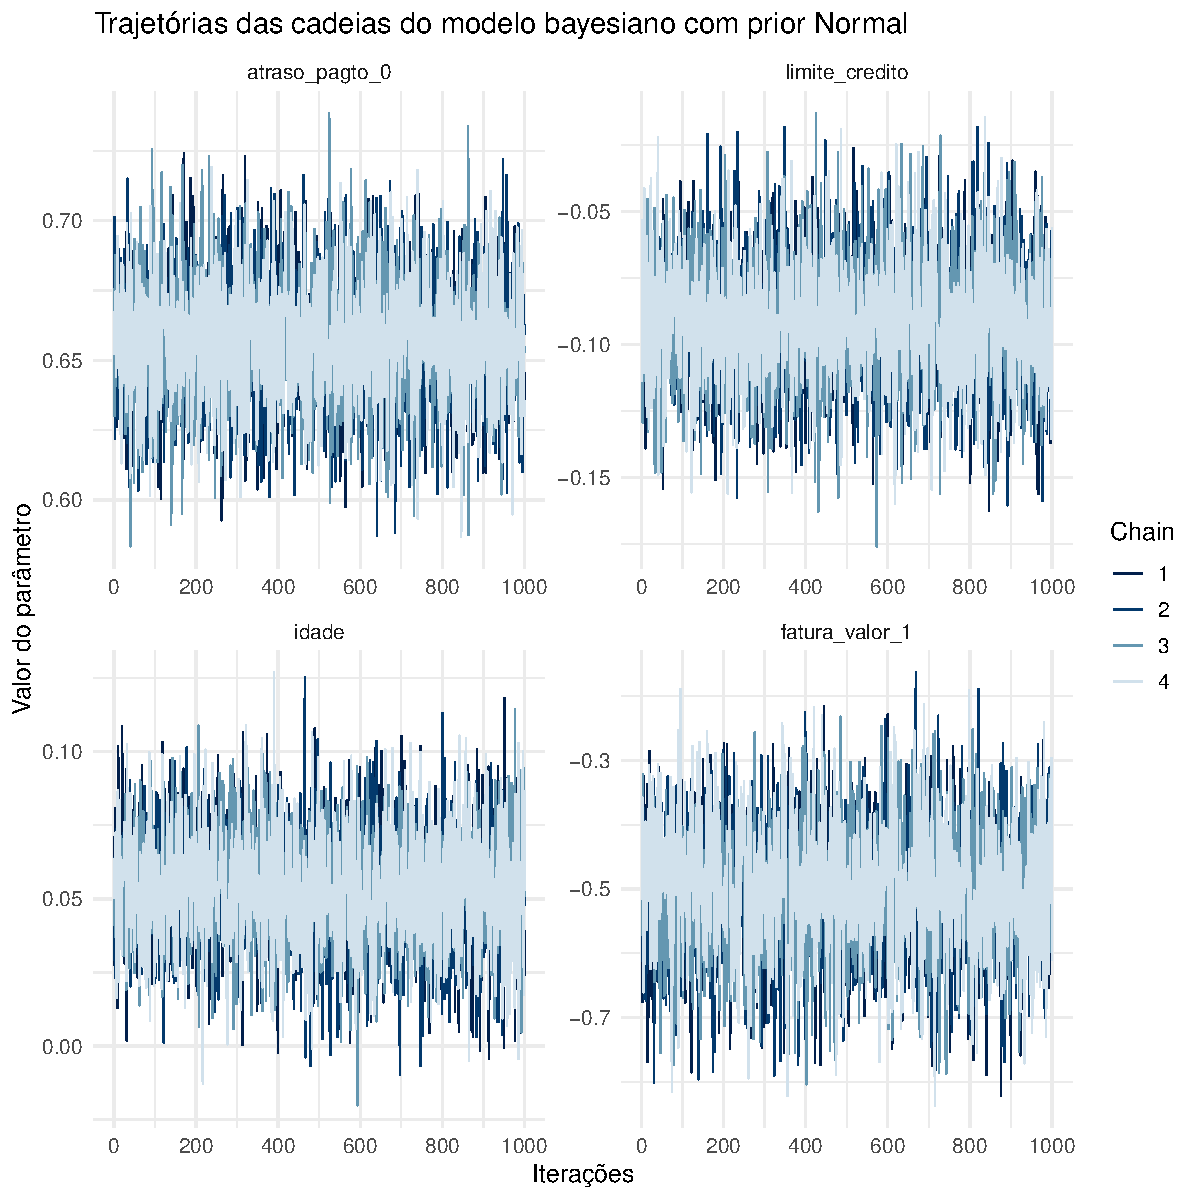
\includegraphics[width=1\linewidth,height=\textheight,keepaspectratio]{monografia_v2_files/figure-pdf/fig-trace-normal-1.pdf}

}

\caption{\label{fig-trace-normal}Gráficos de traço das cadeias de Markov
Monte Carlo (MCMC) para os coeficientes selecionados do modelo bayesiano
com priori Normal.}

\end{figure}%

A inspeção dos \emph{traceplots} (Figura~\ref{fig-trace-normal}) revelou
boa sobreposição entre as quatro cadeias, com oscilações estáveis ao
longo das iterações e ausência de tendências persistentes ou padrões de
separação, indicando mistura adequada e estacionariedade da amostragem.

\begin{figure}

\centering{

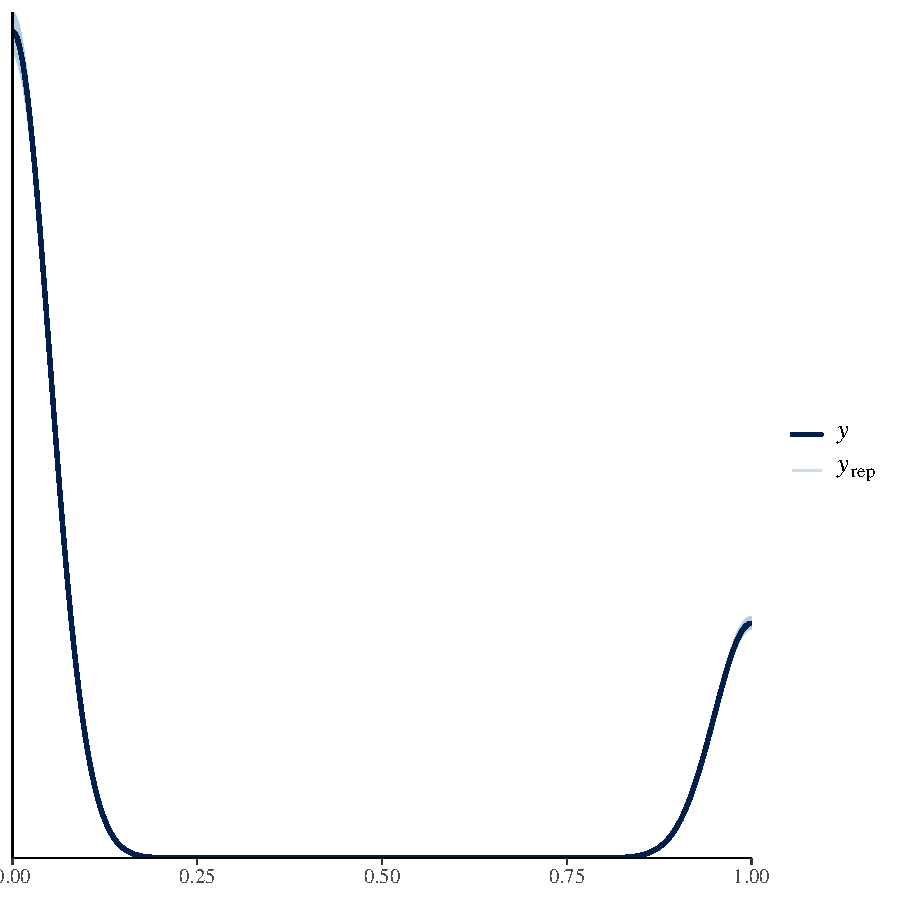
\includegraphics[width=0.65\linewidth,height=\textheight,keepaspectratio]{monografia_v2_files/figure-pdf/fig-pp-check-normal-1.pdf}

}

\caption{\label{fig-pp-check-normal}Verificação preditiva posterior para
o modelo bayesiano com priori Normal}

\end{figure}%

A PPC (Figura~\ref{fig-pp-check-normal}) apresentou sobreposição
satisfatória entre as distribuições observada e replicada para ambas as
categorias, indicando que o modelo reproduz adequadamente a distribuição
marginal da variável resposta, incluindo o desbalanceamento entre as
classes. Essa verificação não atesta a capacidade discriminativa nem a
qualidade das probabilidades individuais, que serão avaliadas pelas
métricas de classificação.

Em conjunto, os diagnósticos indicam convergência satisfatória e
ausência de problemas relevantes no procedimento de amostragem, tornando
as amostras posteriores adequadas para a análise dos parâmetros e do
desempenho preditivo do modelo.

\subparagraph{Priori Laplace}\label{priori-laplace-1}

\begin{table}

\caption{\label{tbl-diagnostics-laplace}Diagnósticos de convergência do
modelo bayesiano com prior Laplace.}

\centering{

\centering\begingroup\fontsize{9}{11}\selectfont

\begin{tabular}{lr}
\toprule
Diagnóstico & Resultado\\
\midrule
Rhat mínimo & 1.000\\
Rhat máximo & 1.003\\
ESS mínimo & 2363.451\\
ESS máximo & 5055.712\\
ESS do log-posterior & 855.478\\
\addlinespace
MCSE do log-posterior & 0.252\\
\bottomrule
\end{tabular}
\endgroup{}

}

\end{table}%

A avaliação da convergência do modelo bayesiano com priori Laplace foi
realizada por meio de diagnósticos numéricos e da verificação do
comportamento das cadeias de Markov. Conforme apresentado na
Tabela~\ref{tbl-diagnostics-laplace}, os valores do fator de redução
potencial de escala \((\hat{R})\) variaram entre 1,000 e 1,003,
indicando concordância entre as cadeias e ausência de evidências de
problemas de convergência. Os tamanhos efetivos da amostra (ESS) dos
coeficientes variaram entre 2.363 e 5.056, demonstrando que, apesar da
autocorrelação inerente às amostras obtidas por métodos de Monte Carlo
via Cadeias de Markov, foi possível obter uma quantidade satisfatória de
amostras efetivamente independentes para a estimação dos parâmetros.

O parâmetro associado ao log-posterior apresentou ESS de 855,478 e erro
padrão de Monte Carlo (MCSE) de 0,252. Embora esses indicadores sejam
menos favoráveis em comparação aos observados para os coeficientes, não
constituem, isoladamente, evidências de problemas de convergência,
devendo ser interpretados em conjunto com os demais diagnósticos.

Os diagnósticos específicos do algoritmo HMC não identificaram
transições divergentes nem saturação da profundidade máxima da árvore de
amostragem, e o E-BFMI não indicou comportamento patológico, resultados
análogos aos observados para o modelo com priori Normal.

\begin{figure}

\centering{

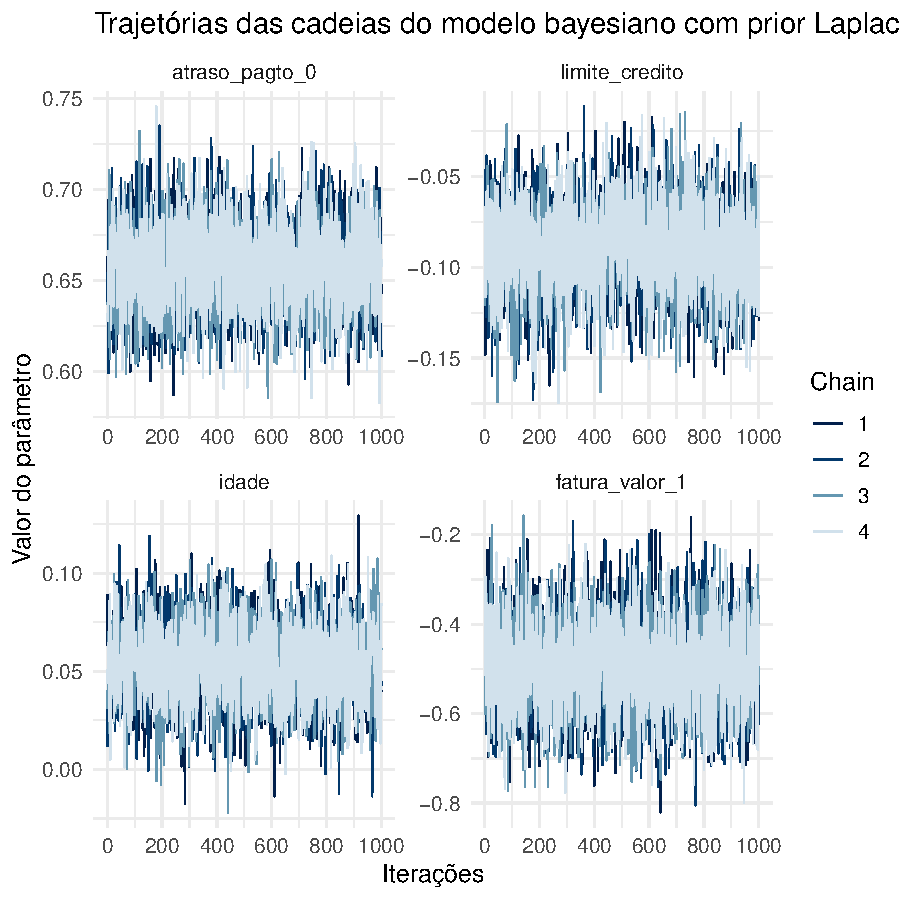
\includegraphics[width=0.75\linewidth,height=\textheight,keepaspectratio]{monografia_v2_files/figure-pdf/fig-trace-laplace-1.pdf}

}

\caption{\label{fig-trace-laplace}Gráficos de traço das cadeias de
Markov Monte Carlo (MCMC) para os coeficientes selecionados do modelo
bayesiano com priori Laplace}

\end{figure}%

A inspeção dos \emph{traceplots} (Figura~\ref{fig-trace-laplace})
evidenciou comportamento semelhante ao observado para o modelo com
priori Normal: as quatro cadeias apresentaram boa sobreposição e
oscilações estáveis ao longo das iterações, sem tendências persistentes
nem padrões de separação, resultado consistente com os diagnósticos
numéricos da Tabela~\ref{tbl-diagnostics-laplace}.

\begin{figure}

\centering{

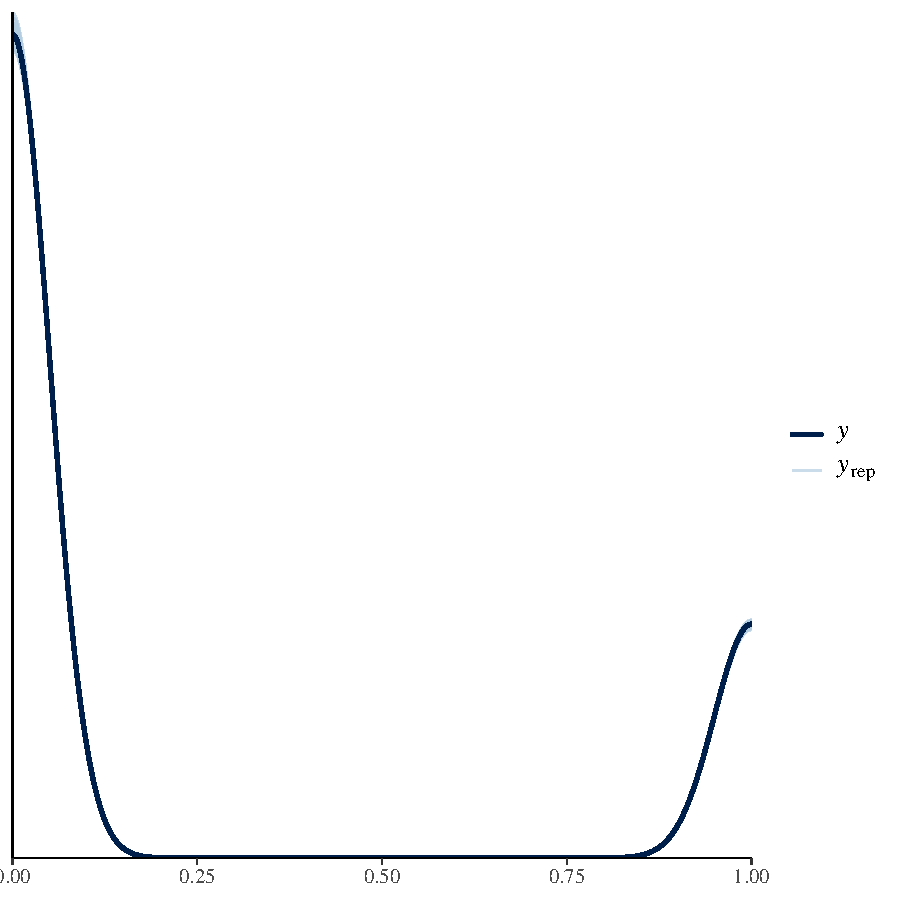
\includegraphics[width=0.65\linewidth,height=\textheight,keepaspectratio]{monografia_v2_files/figure-pdf/fig-pp-check-laplace-1.pdf}

}

\caption{\label{fig-pp-check-laplace}Verificação preditiva posterior
para o modelo bayesiano com priori Laplace}

\end{figure}%

A verificação preditiva posterior (Figura~\ref{fig-pp-check-laplace})
apresentou resultados análogos aos do modelo com priori Normal: boa
sobreposição entre a distribuição observada e as replicações
posteriores, indicando que o modelo reproduz adequadamente a
distribuição marginal da variável resposta.

\paragraph{Comparação entre as especificações
bayesianas}\label{comparauxe7uxe3o-entre-as-especificauxe7uxf5es-bayesianas}

{

\begin{longtable}[]{@{}lrr@{}}

\caption{\label{tbl-waic-comparacao}Comparação dos modelos bayesianos
com base na diferença de ELPD.}

\tabularnewline

\toprule\noalign{}
Modelo & Diferença de ELPD & Erro-padrão da diferença \\
\midrule\noalign{}
\endhead
\bottomrule\noalign{}
\endlastfoot
fit\_laplace & 0.00 & 0.00 \\
fit\_normal & -0.74 & 0.32 \\

\end{longtable}

}

Após a avaliação individual dos modelos bayesianos com priors Normal e
Laplace, realizou-se uma comparação complementar de seu desempenho
preditivo por meio do WAIC. Para essa finalidade, utilizou-se a
diferença de densidade preditiva esperada (ELPD) entre os modelos,
conforme apresentado na Tabela~\ref{tbl-waic-comparacao}.

A comparação tomou o modelo com prior Laplace como referência. Esse
modelo apresentou WAIC de 20.864,79, ligeiramente inferior ao valor de
20.865,83 obtido pelo modelo com prior Normal. Na comparação baseada na
ELPD, o modelo Normal apresentou diferença de −0,74, com erro-padrão de
0,32. Embora os resultados indiquem uma pequena vantagem relativa do
modelo Laplace, a magnitude reduzida da diferença não sugere uma
superioridade preditiva expressiva. Além disso, os valores de
complexidade efetiva \((p_{\text{WAIC}})\) foram próximos entre as
especificações, reforçando a semelhança entre os modelos segundo esse
critério.

\paragraph{Análise das distribuições a
posteriori}\label{anuxe1lise-das-distribuiuxe7uxf5es-a-posteriori}

{

\begin{longtable}[]{@{}
  >{\raggedright\arraybackslash}p{(\linewidth - 12\tabcolsep) * \real{0.1957}}
  >{\raggedleft\arraybackslash}p{(\linewidth - 12\tabcolsep) * \real{0.1232}}
  >{\raggedleft\arraybackslash}p{(\linewidth - 12\tabcolsep) * \real{0.1304}}
  >{\raggedleft\arraybackslash}p{(\linewidth - 12\tabcolsep) * \real{0.1304}}
  >{\raggedleft\arraybackslash}p{(\linewidth - 12\tabcolsep) * \real{0.1377}}
  >{\raggedleft\arraybackslash}p{(\linewidth - 12\tabcolsep) * \real{0.1377}}
  >{\raggedleft\arraybackslash}p{(\linewidth - 12\tabcolsep) * \real{0.1449}}@{}}

\caption{\label{tbl-resumo-posterior}Medianas e intervalos de
credibilidade de 95\% dos coeficientes dos modelos bayesianos com
prioris Normal e Laplace.}

\tabularnewline

\toprule\noalign{}
\begin{minipage}[b]{\linewidth}\raggedright
Variável
\end{minipage} & \begin{minipage}[b]{\linewidth}\raggedleft
Mediana (Normal)
\end{minipage} & \begin{minipage}[b]{\linewidth}\raggedleft
Mediana (Laplace)
\end{minipage} & \begin{minipage}[b]{\linewidth}\raggedleft
ICr 2,5\% (Normal)
\end{minipage} & \begin{minipage}[b]{\linewidth}\raggedleft
ICr 97,5\% (Normal)
\end{minipage} & \begin{minipage}[b]{\linewidth}\raggedleft
ICr 2,5\% (Laplace)
\end{minipage} & \begin{minipage}[b]{\linewidth}\raggedleft
ICr 97,5\% (Laplace)
\end{minipage} \\
\midrule\noalign{}
\endhead
\bottomrule\noalign{}
\endlastfoot
(Intercept) & -1.484 & -1.483 & -1.523 & -1.445 & -1.522 & -1.444 \\
atraso\_pagto\_0 & 0.657 & 0.657 & 0.614 & 0.701 & 0.614 & 0.702 \\
atraso\_pagto\_2 & 0.094 & 0.093 & 0.039 & 0.151 & 0.039 & 0.150 \\
atraso\_pagto\_3 & 0.083 & 0.083 & 0.020 & 0.144 & 0.022 & 0.142 \\
atraso\_pagto\_4 & 0.053 & 0.051 & -0.013 & 0.118 & -0.015 & 0.115 \\
atraso\_pagto\_5 & 0.031 & 0.033 & -0.038 & 0.099 & -0.032 & 0.100 \\
atraso\_pagto\_6 & 0.001 & 0.003 & -0.056 & 0.059 & -0.055 & 0.057 \\
escolaridade\_Desconhecido1 & -0.183 & -0.179 & -0.257 & -0.118 & -0.253
& -0.118 \\
escolaridade\_Desconhecido2 & 0.001 & 0.000 & -0.038 & 0.035 & -0.039 &
0.035 \\
escolaridade\_EnsinoMedio & -0.046 & -0.044 & -0.085 & -0.006 & -0.084 &
-0.005 \\
escolaridade\_Outros & -0.066 & -0.064 & -0.125 & -0.017 & -0.126 &
-0.013 \\
escolaridade\_Universidade & -0.038 & -0.037 & -0.077 & 0.002 & -0.078 &
0.005 \\
estado\_civil\_Outros & -0.011 & -0.011 & -0.046 & 0.021 & -0.045 &
0.021 \\
estado\_civil\_Solteiro & -0.089 & -0.089 & -0.127 & -0.051 & -0.127 &
-0.049 \\
fatura\_valor\_1 & -0.503 & -0.487 & -0.708 & -0.311 & -0.684 &
-0.295 \\
fatura\_valor\_2 & 0.277 & 0.255 & 0.037 & 0.522 & 0.031 & 0.497 \\
fatura\_valor\_3 & 0.048 & 0.048 & -0.156 & 0.263 & -0.146 & 0.244 \\
fatura\_valor\_4 & -0.021 & -0.021 & -0.223 & 0.174 & -0.207 & 0.172 \\
fatura\_valor\_5 & 0.109 & 0.098 & -0.107 & 0.322 & -0.097 & 0.303 \\
fatura\_valor\_6 & -0.005 & 0.002 & -0.166 & 0.163 & -0.155 & 0.164 \\
idade & 0.053 & 0.053 & 0.014 & 0.092 & 0.015 & 0.091 \\
limite\_credito & -0.091 & -0.090 & -0.137 & -0.045 & -0.138 & -0.043 \\
pagto\_valor\_1 & -0.229 & -0.225 & -0.322 & -0.148 & -0.311 & -0.146 \\
pagto\_valor\_2 & -0.184 & -0.183 & -0.288 & -0.093 & -0.282 & -0.092 \\
pagto\_valor\_3 & -0.035 & -0.036 & -0.105 & 0.032 & -0.105 & 0.026 \\
pagto\_valor\_4 & -0.093 & -0.091 & -0.163 & -0.031 & -0.162 & -0.028 \\
pagto\_valor\_5 & -0.062 & -0.061 & -0.128 & -0.001 & -0.131 & -0.002 \\
pagto\_valor\_6 & -0.048 & -0.048 & -0.105 & 0.005 & -0.108 & 0.004 \\
sexo\_Feminino & -0.067 & -0.067 & -0.101 & -0.032 & -0.101 & -0.034 \\

\end{longtable}

}

A comparação das distribuições posteriores evidencia resultados bastante
semelhantes entre os modelos especificados com prioris Normal e Laplace.
As medianas dos coeficientes apresentam diferenças pequenas, assim como
os respectivos intervalos de credibilidade de 95\%, conforme apresentado
na Tabela~\ref{tbl-resumo-posterior}. Esse comportamento sugere que,
para a amostra e as especificações consideradas, as estimativas
posteriores são pouco sensíveis à escolha entre essas duas distribuições
a priori.

Cabe destacar que os preditores foram padronizados antes do ajuste dos
modelos, incluindo as variáveis indicadoras binárias geradas a partir
das variáveis categóricas. Dessa forma, os coeficientes representam
variações no logaritmo das chances (\emph{log-odds}) de inadimplência
associadas ao aumento de um desvio-padrão no respectivo preditor
transformado, mantendo-se os demais constantes. Consequentemente, a
interpretação dos coeficientes das variáveis indicadoras, como
\texttt{sexo\_Feminino}, deve considerar essa transformação, não
correspondendo diretamente à comparação entre as categorias na escala
original.

Entre os coeficientes estimados, destacam-se aqueles associados às
variáveis \texttt{atraso\_pagto\_0}, \texttt{atraso\_pagto\_2},
\texttt{atraso\_pagto\_3}, \texttt{fatura\_valor\_1},
\texttt{fatura\_valor\_2} e \texttt{idade}, cujos intervalos de
credibilidade de 95\% não incluem zero em ambas as especificações.
Também se observam associações negativas para \texttt{limite\_credito},
\texttt{pagto\_valor\_1}, \texttt{pagto\_valor\_2} e
\texttt{sexo\_Feminino}, cujos intervalos também permanecem abaixo de
zero nas duas especificações. A concordância entre os modelos quanto à
direção desses efeitos reforça a proximidade das estimativas obtidas sob
as diferentes distribuições a priori.

Por outro lado, variáveis como \texttt{atraso\_pagto\_4},
\texttt{atraso\_pagto\_5}, \texttt{atraso\_pagto\_6} e
\texttt{fatura\_valor\_3} apresentam intervalos de credibilidade que
incluem zero, indicando maior incerteza quanto à direção de seus
efeitos. Esse resultado evidencia que nem todos os coeficientes
apresentam o mesmo grau de concentração nas distribuições posteriores.

De modo geral, não se observam diferenças expressivas no comportamento
dos coeficientes entre os modelos Normal e Laplace. Embora as
distribuições a priori possuam formatos distintos, suas variâncias foram
igualadas para tornar a comparação mais controlada, permitindo avaliar
os efeitos associados às diferenças em suas formas. Para os dados e as
especificações analisados, essas diferenças não produziram alterações
substanciais nas estimativas posteriores.

\begin{figure}

\centering{

\pandocbounded{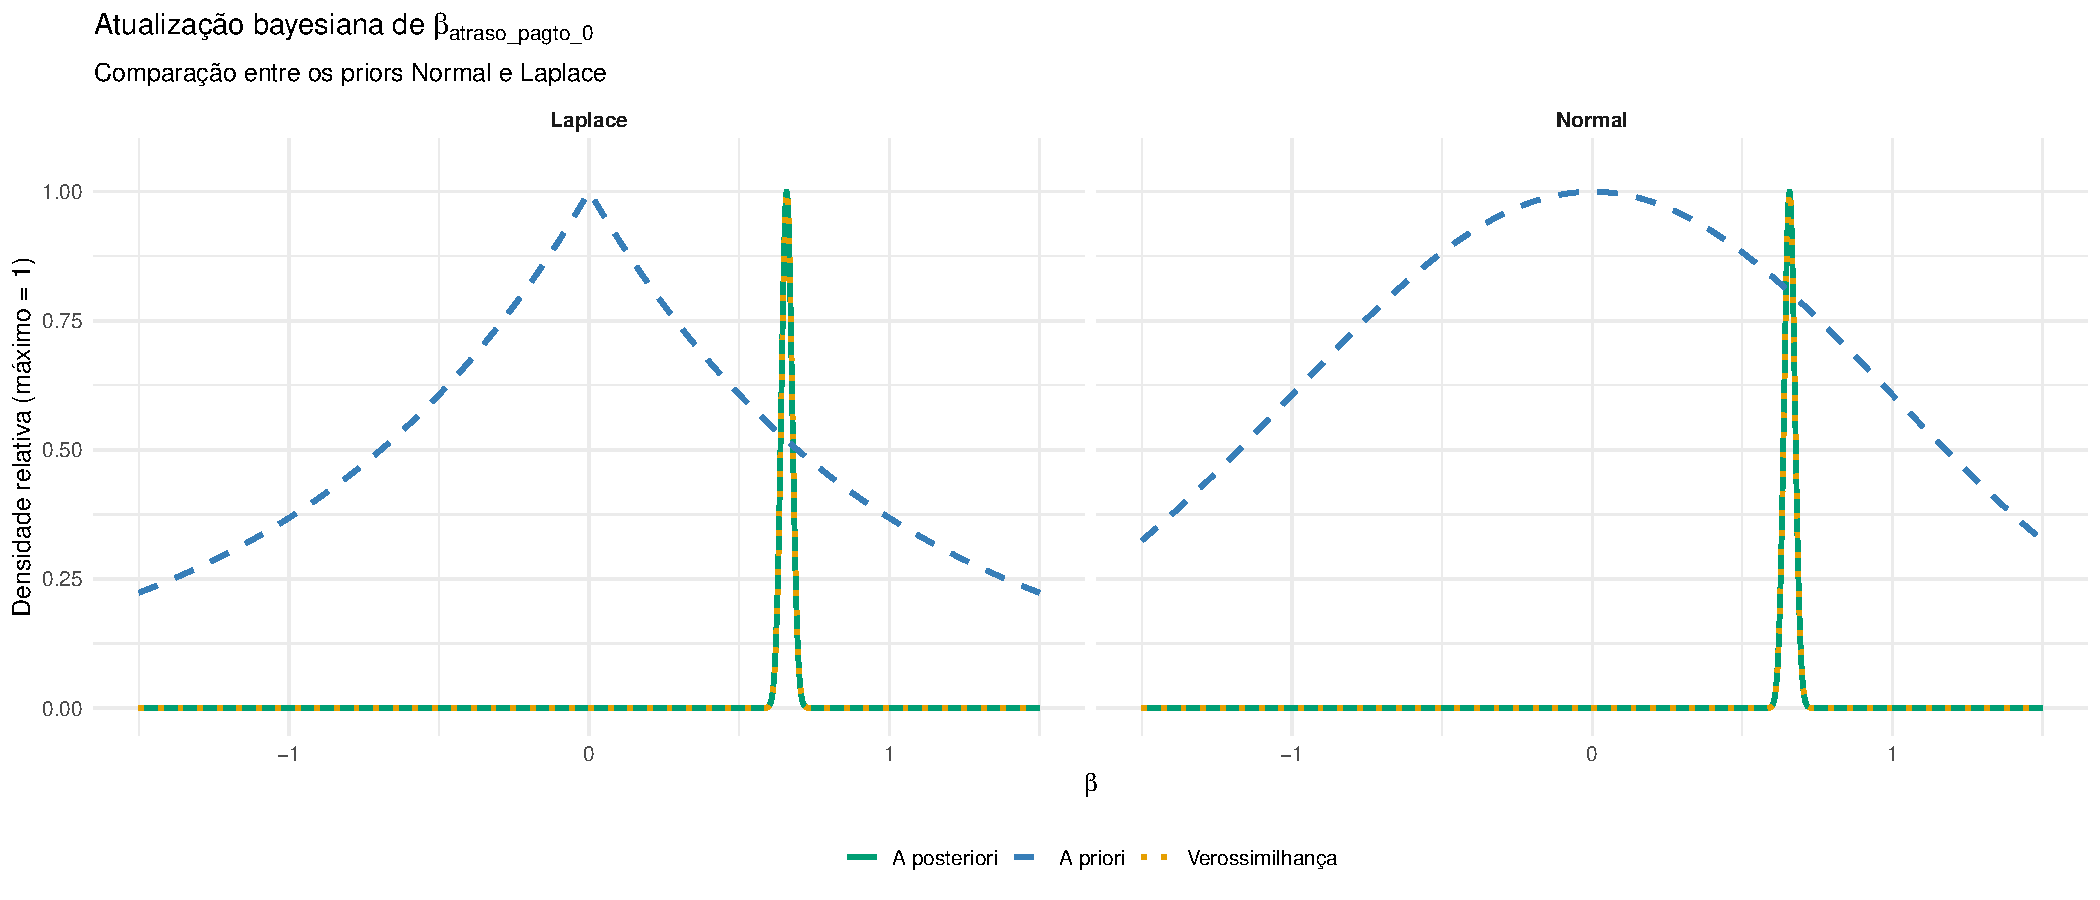
\includegraphics[keepaspectratio]{monografia_v2_files/figure-pdf/fig-atualizacao-bayesiana-pgto-1.pdf}}

}

\caption{\label{fig-atualizacao-bayesiana-pgto}Atualização bayesiana do
coeficiente de atraso\_pagto\_0: comparação entre os priors Normal e
Laplace.}

\end{figure}%

A Figura~\ref{fig-atualizacao-bayesiana-pgto} apresenta uma
representação da atualização bayesiana do coeficiente associado à
variável \texttt{atraso\_pagto\_0}, considerando as especificações com
priors Normal e Laplace. Em ambos os painéis, são apresentadas as
distribuições a priori, as funções de verossimilhança condicionais e as
distribuições a posteriori, permitindo visualizar a contribuição da
informação inicial e dos dados para a estimação do parâmetro.

Observa-se que as distribuições a priori possuem formatos distintos,
decorrentes das propriedades das distribuições Normal e Laplace.
Entretanto, a incorporação da informação amostral conduz a distribuições
a posteriori bastante semelhantes, concentradas em torno de valores
positivos do coeficiente.

Além disso, nota-se visualmente que a função de verossimilhança possui
uma dispersão extremamente restrita em comparação às distribuições a
priori, concentrando seu máximo próximo a \(\beta \approx 0.7\). Essa
alta precisão amostral faz com que a distribuição a posteriori seja
quase integralmente moldada pelos dados, sobrepondo-se à verossimilhança
e atenuando de forma expressiva a influência inicial das especificações
Normal e Laplace.

A concentração das distribuições a posteriori em uma região
relativamente estreita indica que, para esse preditor, a informação
fornecida pelos dados exerce papel importante na estimação do
coeficiente. Assim, apesar das diferenças entre as distribuições a
priori, ambas as especificações conduzem a resultados semelhantes após a
atualização.

Ressalta-se que a verossimilhança apresentada corresponde a uma
avaliação condicional, na qual os demais coeficientes foram mantidos
fixos em suas medianas posteriores. Além disso, as curvas foram
reescaladas para que seus valores máximos fossem iguais a um, de modo a
facilitar a comparação visual de seus formatos. Portanto, a figura
possui finalidade ilustrativa e não representa as distribuições
marginais completas dos parâmetros.

\subparagraph{Interpretação dos coeficientes e das razões de
chances}\label{interpretauxe7uxe3o-dos-coeficientes-e-das-razuxf5es-de-chances}

Na regressão logística, os coeficientes representam a variação no
logaritmo das chances (\emph{log-odds}) de ocorrência do evento de
interesse, neste caso, a inadimplência ((PD30 = 1)), associada ao
aumento de uma unidade no preditor, mantendo-se os demais constantes.
Como as variáveis explicativas foram padronizadas antes do ajuste dos
modelos, inclusive as variáveis indicadoras binárias, essa interpretação
deve considerar a escala padronizada dos preditores. Assim, para as
variáveis numéricas, o aumento de uma unidade corresponde a um
desvio-padrão na escala original.

Coeficientes positivos indicam associação com o aumento das chances de
inadimplência, enquanto coeficientes negativos indicam associação com
sua redução. A magnitude dos coeficientes expressa a intensidade dessas
associações na escala do logaritmo das chances.

Conforme apresentado na Tabela~\ref{tbl-resumo-posterior}, os modelos
com prioris Normal e Laplace apresentam estimativas bastante próximas,
sugerindo que a escolha entre essas duas distribuições a priori não
produziu alterações expressivas nas conclusões sobre os efeitos dos
preditores.

Entre os coeficientes positivos, destaca-se \texttt{atraso\_pagto\_0},
com mediana posterior de 0,657 em ambas as especificações. Esse preditor
apresenta a maior estimativa positiva entre as variáveis explicativas,
com intervalo de credibilidade de 95\% inteiramente acima de zero.
Também apresentam associações positivas \texttt{atraso\_pagto\_2},
\texttt{atraso\_pagto\_3}, \texttt{fatura\_valor\_2} e \texttt{idade},
cujos intervalos de credibilidade também não incluem zero.

Por outro lado, \texttt{fatura\_valor\_1} apresenta a maior estimativa
negativa, com medianas posteriores de -0,503 no modelo Normal e -0,487
no modelo Laplace. Outros efeitos negativos são observados para
\texttt{pagto\_valor\_1}, \texttt{pagto\_valor\_2} e
\texttt{limite\_credito}. Também se destacam
\texttt{escolaridade\_Desconhecido1},
\texttt{escolaridade\_EnsinoMedio}, \texttt{escolaridade\_Outros},
\texttt{estado\_civil\_Solteiro} e \texttt{sexo\_Feminino}, cujos
intervalos de credibilidade de 95\% permanecem abaixo de zero nas duas
especificações.

Para facilitar a interpretação dos efeitos estimados na regressão
logística, os coeficientes podem ser exponenciados, obtendo-se as razões
de chances (\emph{Odds Ratios}, OR). Essa transformação permite
expressar os efeitos em termos multiplicativos sobre as chances de
inadimplência:

\(OR_j = \exp(\beta_j).\)

Valores de OR superiores a 1 indicam aumento nas chances de
inadimplência, enquanto valores inferiores a 1 indicam redução. Um OR
igual a 1 corresponde à ausência de associação na escala das chances.

Considerando as medianas posteriores, o preditor
\texttt{atraso\_pagto\_0} apresenta OR de aproximadamente 1,929 em ambas
as especificações. Isso indica que um aumento de uma unidade na escala
padronizada desse preditor está associado a chances de inadimplência
aproximadamente 92,9\% maiores, mantendo-se os demais preditores
constantes. Entre os demais efeitos positivos, destacam-se
\texttt{atraso\_pagto\_2}, com OR próximo de 1,099 no modelo Normal e
1,098 no Laplace; \texttt{atraso\_pagto\_3}, com OR próximo de 1,087;
\texttt{fatura\_valor\_2}, com OR de aproximadamente 1,319 no modelo
Normal e 1,290 no Laplace; e \texttt{idade}, com OR próximo de 1,054.

Em relação aos efeitos negativos, \texttt{fatura\_valor\_1} apresenta OR
de aproximadamente 0,605 no modelo Normal e 0,614 no Laplace. Esses
valores correspondem a reduções de cerca de 39,5\% e 38,6\% nas chances
de inadimplência, respectivamente, para um aumento de uma unidade na
escala padronizada do preditor. Também se destacam
\texttt{pagto\_valor\_1}, com OR próximo de 0,795 no modelo Normal e
0,798 no Laplace; \texttt{pagto\_valor\_2}, com OR próximo de 0,832 e
0,833, respectivamente; e \texttt{limite\_credito}, com OR próximo de
0,913 e 0,914.

A comparação entre os modelos evidencia que os ORs obtidos são bastante
semelhantes. As pequenas diferenças observadas nas estimativas não
alteram a direção dos efeitos nem a identificação dos principais
preditores associados à inadimplência.

Ressalta-se que os ORs apresentados foram calculados a partir das
medianas posteriores dos coeficientes e se referem a variações de uma
unidade na escala padronizada dos preditores. Portanto, não devem ser
interpretados diretamente como alterações associadas a uma unidade
monetária, a um ano de idade ou à mudança entre categorias originais das
variáveis indicadoras. No caso destas últimas, a interpretação também
deve considerar a padronização: o coeficiente não representa diretamente
a comparação entre as categorias originais, mas a variação associada a
uma unidade na escala transformada da variável.

\subparagraph{Intervalos de credibilidade e incerteza das
estimativas}\label{intervalos-de-credibilidade-e-incerteza-das-estimativas}

Os intervalos de credibilidade de 95\% permitem avaliar a incerteza
associada às estimativas dos coeficientes, indicando uma faixa de
valores que contém 95\% da probabilidade posterior do parâmetro,
condicionada aos dados observados e à distribuição a priori adotada.
Diferentemente dos intervalos de confiança frequentistas, sua
interpretação está diretamente relacionada à distribuição posterior do
parâmetro.

A análise dos intervalos de credibilidade
(Tabela~\ref{tbl-resumo-posterior}) mostra que 16 dos 27 preditores
apresentam intervalos inteiramente fora de zero em ambas as
especificações, confirmando as direções de efeito identificadas na
subseção anterior. Os coeficientes mais bem determinados, como
\texttt{atraso\_pagto\_0}, apresentam intervalos relativamente
estreitos; variáveis como \texttt{fatura\_valor\_2} a
\texttt{fatura\_valor\_5} exibem maior dispersão posterior, indicando
maior incerteza sobre a magnitude de seus efeitos. A proximidade entre
os limites dos intervalos dos modelos Normal e Laplace indica que a
incerteza das estimativas foi semelhante sob as duas especificações de
prioris.

\paragraph{Avaliação do desempenho
preditivo}\label{avaliauxe7uxe3o-do-desempenho-preditivo}

\begin{table}

\caption{\label{tbl-results-all}Métricas de desempenho dos modelos de
regressão logística bayesiano e frequentista para previsão de PD30 no
conjunto de teste.}

\centering{

\centering\begingroup\fontsize{8}{10}\selectfont

\begin{tabular}{lrrrrrr}
\toprule
Métrica & Completo & Sem multicol. & L1 (LASSO) & L2 (Ridge) & Bayesiano (Laplace) & Bayesiano (Normal)\\
\midrule
Acurácia & 0.8105 & 0.8117 & 0.8108 & 0.8069 & 0.8105 & 0.8105\\
Acurácia balanceada & 0.6129 & 0.6135 & 0.6129 & 0.5990 & 0.6127 & 0.6129\\
ROC AUC & 0.7163 & 0.7141 & 0.7161 & 0.7153 & 0.7164 & 0.7165\\
Log-loss & 0.4702 & 0.4698 & 0.4699 & 0.4695 & 0.4699 & 0.4699\\
Sensibilidade & 0.2586 & 0.2580 & 0.2580 & 0.2260 & 0.2580 & 0.2586\\
\addlinespace
Especificidade & 0.9673 & 0.9690 & 0.9678 & 0.9719 & 0.9675 & 0.9673\\
Precisão & 0.6919 & 0.7028 & 0.6948 & 0.6957 & 0.6926 & 0.6919\\
F1-score & 0.3765 & 0.3774 & 0.3763 & 0.3412 & 0.3759 & 0.3765\\
MCC & 0.3405 & 0.3449 & 0.3413 & 0.3181 & 0.3403 & 0.3405\\
\bottomrule
\end{tabular}
\endgroup{}

}

\end{table}%

A avaliação do desempenho preditivo dos modelos foi realizada com base
em métricas calculadas sobre o conjunto de teste, permitindo comparar a
capacidade de generalização das abordagens frequentista e bayesiana.
Foram consideradas métricas relacionadas à classificação, à
discriminação entre as classes e à qualidade das probabilidades
estimadas, de modo a proporcionar uma avaliação mais abrangente do
desempenho dos modelos (Tabela~\ref{tbl-results-all}).

De maneira geral, os resultados evidenciam elevada proximidade entre os
modelos avaliados. A acurácia variou entre 0,8069 e 0,8117, indicando
que aproximadamente 81\% das observações foram classificadas
corretamente. Entre as especificações, o modelo frequentista sem
multicolinearidade apresentou o maior valor (0,8117), enquanto o modelo
Ridge apresentou o menor (0,8069). Os modelos bayesianos, por sua vez,
alcançaram acurácia de 0,8105 em ambas as especificações, demonstrando
desempenho bastante semelhante ao das alternativas frequentistas.

Entretanto, a interpretação da acurácia deve considerar o
desbalanceamento da variável resposta. Aproximadamente 78\% das
observações pertencem à classe 0, enquanto cerca de 22\% correspondem à
classe 1. Nesse cenário, a acurácia convencional pode superestimar a
qualidade da classificação, uma vez que o desempenho sobre a classe
majoritária exerce maior influência sobre seu valor. Essa limitação
também pode ser observada nos resultados da acurácia balanceada, que
variaram entre 0,5990 e 0,6135. A diferença entre as duas medidas indica
que, apesar da proporção relativamente elevada de classificações
corretas, os modelos apresentam desempenho desigual na identificação das
duas classes.

A análise da sensibilidade e da especificidade reforça essa constatação.
Os valores de sensibilidade, entre 0,2260 e 0,2586, revelam uma
capacidade limitada de identificar corretamente os clientes
inadimplentes. Em contrapartida, a especificidade variou entre 0,9673 e
0,9719, indicando que os modelos identificaram corretamente a grande
maioria dos clientes não inadimplentes. Esse comportamento evidencia uma
tendência dos classificadores a favorecer a atribuição da classe
negativa, resultando em um número expressivo de falsos negativos e em
uma proporção reduzida de inadimplentes corretamente identificados.

A precisão apresentou valores entre 0,6919 e 0,7028, indicando que
aproximadamente 69\% a 70\% das observações classificadas como
inadimplentes pertencem efetivamente a essa categoria. O F1-score, por
sua vez, variou entre 0,3412 e 0,3774. Por combinar precisão e
sensibilidade por meio da média harmônica, essa métrica também evidencia
as limitações dos modelos na identificação da classe positiva,
especialmente em razão dos baixos valores de sensibilidade.

O MCC apresentou valores entre 0,3181 e 0,3449. Por considerar
simultaneamente os verdadeiros e falsos positivos e negativos, essa
métrica oferece uma perspectiva mais abrangente do desempenho
classificatório, especialmente diante do desbalanceamento observado. Os
valores obtidos indicam uma associação positiva, porém relativamente
limitada, entre as classificações realizadas pelos modelos e as classes
efetivamente observadas.

Em relação à qualidade das probabilidades estimadas, o log-loss
apresentou resultados praticamente idênticos entre as seis
especificações, variando de 0,4695 a 0,4702. Essa proximidade sugere que
as diferentes estratégias de estimação e regularização produziram
probabilidades preditas com qualidade semelhante, sem diferenças
expressivas nessa dimensão do desempenho.

De forma geral, os resultados apontam para uma elevada semelhança entre
as especificações frequentistas e bayesianas quanto ao desempenho
preditivo. As diferenças observadas nas métricas são pequenas, sugerindo
que a incorporação de distribuições a priori, nas configurações
avaliadas, não proporcionou ganhos expressivos em relação às
alternativas frequentistas. Ainda assim, a avaliação evidencia uma
limitação comum aos modelos: a baixa sensibilidade na identificação dos
clientes inadimplentes, apesar da elevada especificidade para a classe
de não inadimplência.

A capacidade discriminatória dos modelos foi analisada adicionalmente
por meio da área sob a curva ROC (ROC AUC), métrica que avalia a
capacidade de distinguir observações pertencentes às diferentes classes
ao longo de diversos pontos de corte. Diferentemente das métricas
baseadas em classificações binárias, essa medida não depende da adoção
de um limiar específico para transformar as probabilidades estimadas em
classes.

Os resultados apresentaram valores próximos entre as especificações
frequentistas e bayesianas. Enquanto os modelos frequentistas
registraram valores de ROC AUC entre 0,7141 e 0,7163, os modelos
bayesianos alcançaram 0,7164 e 0,7165, respectivamente para as prioris
Laplace e Normal. Essa proximidade indica que as diferentes abordagens
produziram capacidades discriminatórias semelhantes, sem evidências de
vantagem expressiva de uma delas.

Embora os modelos bayesianos tenham apresentado valores ligeiramente
superiores, a magnitude dessa diferença é pequena e não permite concluir
que a abordagem bayesiana proporcione uma melhoria relevante na
discriminação entre clientes inadimplentes e não inadimplentes. De
maneira semelhante, as diferenças entre as especificações frequentistas
também foram reduzidas, indicando que as estratégias de regularização e
tratamento da multicolinearidade tiveram efeitos limitados sobre essa
dimensão do desempenho.

Assim, os resultados sugerem que, para o conjunto de dados e as
especificações consideradas, a escolha entre inferência frequentista e
bayesiana não alterou substancialmente a capacidade de ordenação dos
clientes segundo seu risco de inadimplência.

\paragraph{Análise dos erros de
classificação}\label{sec-erros-classificacao}

A Figura~\ref{fig-confusion-matrices} apresenta as matrizes de confusão
dos modelos frequentista (sem multicolinearidade) e bayesiano (priori
Normal), avaliados no conjunto de teste com ponto de corte de 0,5. Os
resultados mostram padrões praticamente idênticos: o frequentista
registrou 1.231 falsos negativos e 181 falsos positivos, enquanto o
bayesiano apresentou 1.230 e 191, respectivamente. Aproximadamente 74\%
dos clientes efetivamente inadimplentes não foram identificados por
nenhum dos modelos, refletindo a baixa sensibilidade
(\textasciitilde25,8\%) já reportada na Tabela~\ref{tbl-results-all} e o
impacto do desbalanceamento da variável resposta.

A predominância de falsos negativos em relação aos falsos positivos
indica que os classificadores tendem a subestimar o risco de
inadimplência --- clientes que efetivamente inadimplirão são
classificados como não inadimplentes, o que pode resultar em concessão
indevida de crédito. A adoção do modelo bayesiano não modificou
substancialmente esse padrão. A definição de um ponto de corte adequado,
considerando os custos relativos de cada tipo de erro e os objetivos
institucionais, é retomada na Discussão.

\begin{verbatim}
  Real Predito Freq                       Modelo
1    0       0 5660 Frequentista (sem multicol.)
2    1       0 1231 Frequentista (sem multicol.)
3    0       1  181 Frequentista (sem multicol.)
4    1       1  428 Frequentista (sem multicol.)
5    0       0 5650           Bayesiano (Normal)
6    1       0 1230           Bayesiano (Normal)
7    0       1  191           Bayesiano (Normal)
8    1       1  429           Bayesiano (Normal)
\end{verbatim}

\begin{figure}

\centering{

\pandocbounded{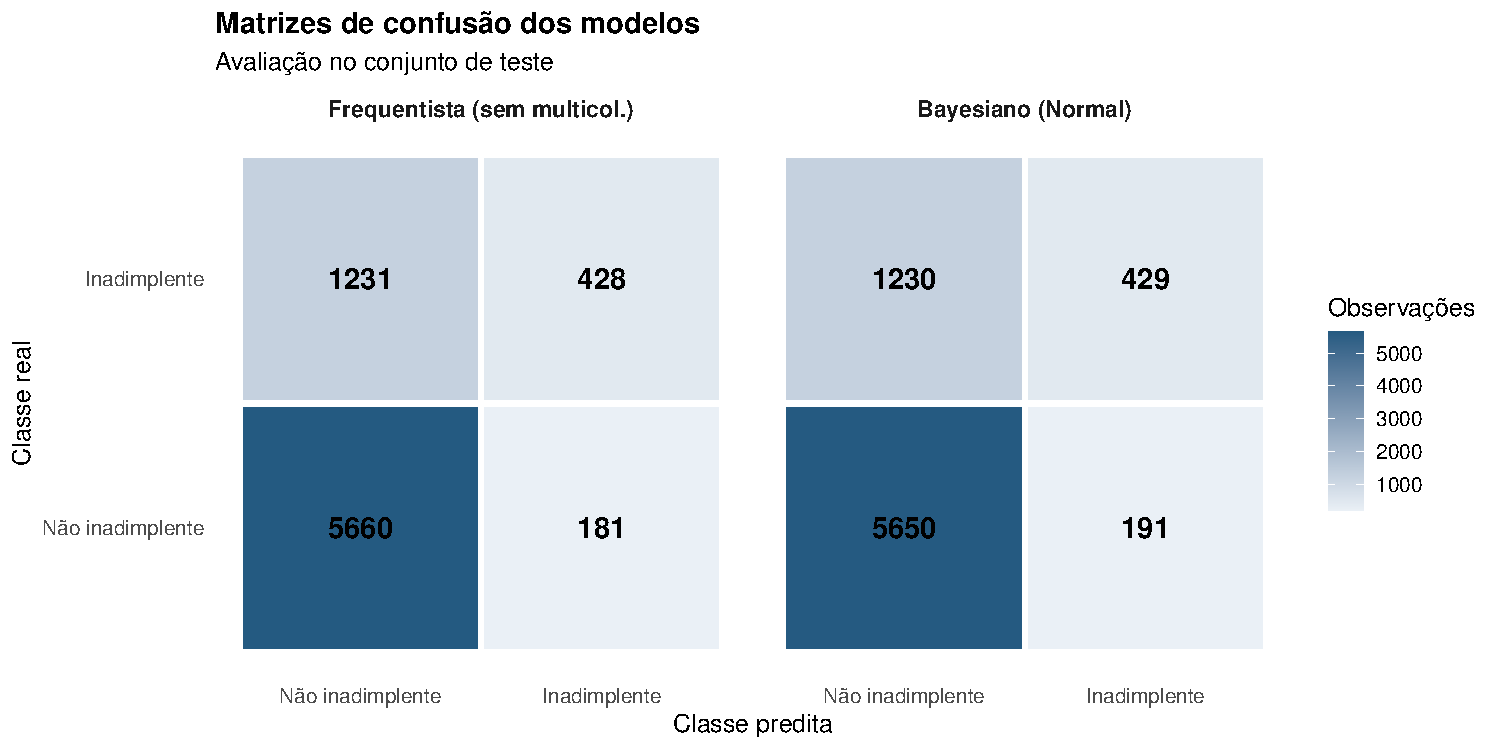
\includegraphics[keepaspectratio]{monografia_v2_files/figure-pdf/fig-confusion-matrices-1.pdf}}

}

\caption{\label{fig-confusion-matrices}Matrizes de confusão dos modelos
frequentista e bayesiano no conjunto de teste.}

\end{figure}%

{

\begin{longtable}[]{@{}
  >{\raggedright\arraybackslash}p{(\linewidth - 8\tabcolsep) * \real{0.3919}}
  >{\raggedleft\arraybackslash}p{(\linewidth - 8\tabcolsep) * \real{0.1486}}
  >{\raggedleft\arraybackslash}p{(\linewidth - 8\tabcolsep) * \real{0.1622}}
  >{\raggedleft\arraybackslash}p{(\linewidth - 8\tabcolsep) * \real{0.1622}}
  >{\raggedleft\arraybackslash}p{(\linewidth - 8\tabcolsep) * \real{0.1351}}@{}}

\caption{\label{tbl-youden}Melhores limites de corte com base no índice
de Youden}

\tabularnewline

\toprule\noalign{}
\begin{minipage}[b]{\linewidth}\raggedright
Modelo
\end{minipage} & \begin{minipage}[b]{\linewidth}\raggedleft
.threshold
\end{minipage} & \begin{minipage}[b]{\linewidth}\raggedleft
sensitivity
\end{minipage} & \begin{minipage}[b]{\linewidth}\raggedleft
specificity
\end{minipage} & \begin{minipage}[b]{\linewidth}\raggedleft
youden
\end{minipage} \\
\midrule\noalign{}
\endhead
\bottomrule\noalign{}
\endlastfoot
Bayesiano (Normal) & 0.2548669 & 0.5623870 & 0.8127033 & 0.3750903 \\
Frequentista (Sem Multicol.) & 0.2625011 & 0.5364678 & 0.8375278 &
0.3739956 \\

\end{longtable}

}

\begin{figure}[H]

{\centering 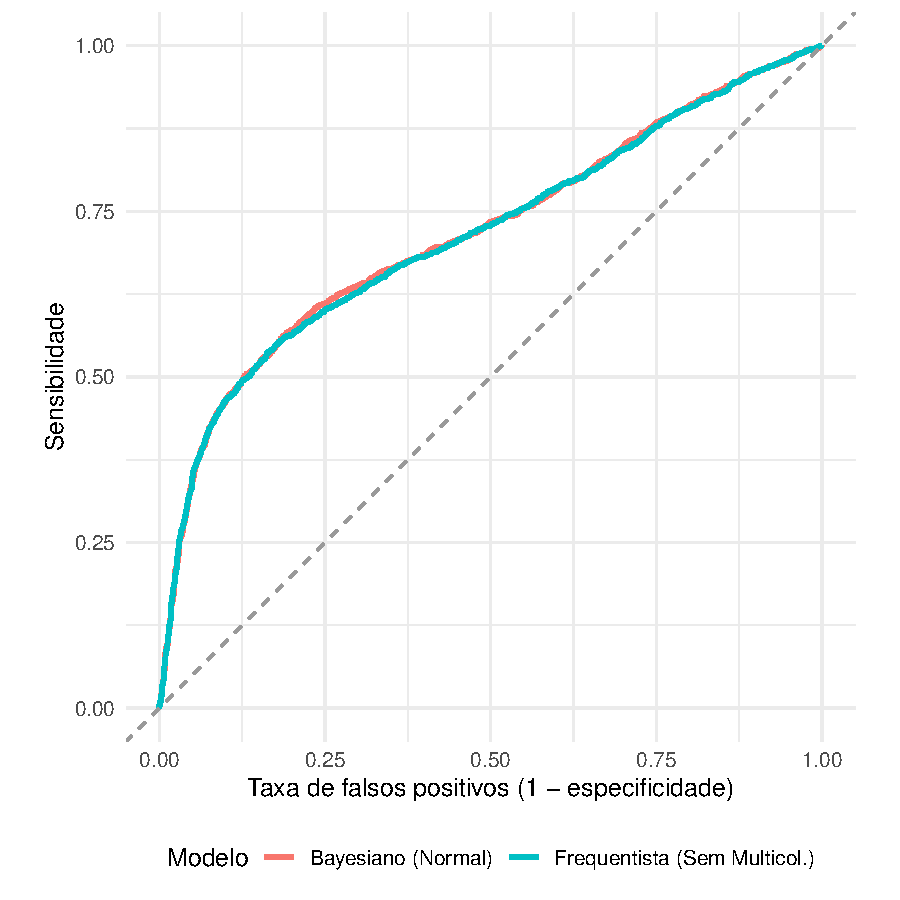
\includegraphics[width=0.65\linewidth,height=\textheight,keepaspectratio]{monografia_v2_files/figure-pdf/roc-comparacao-1.pdf}

}

\caption{Curvas ROC dos modelos frequentista (Sem Multicol.) e bayesiano
(Normal) no conjunto de teste.}

\end{figure}%

\paragraph{Análise das curvas ROC}\label{anuxe1lise-das-curvas-roc}

A (\textbf{roc-comparacao?}) apresenta as curvas ROC dos modelos
frequentista e bayesiano com prior Normal, construídas a partir das
probabilidades estimadas no conjunto de teste. A curva ROC permite
avaliar a capacidade discriminatória dos modelos para diferentes pontos
de corte, relacionando a sensibilidade à taxa de falsos positivos (1 −
especificidade).

Observa-se que as duas curvas apresentam trajetórias bastante próximas e
praticamente sobrepostas ao longo de sua extensão, indicando
comportamento discriminatório semelhante. Esse resultado é consistente
com os valores de AUC, de aproximadamente 0,714 para o modelo
frequentista e 0,716 para o modelo bayesiano. Embora ambos apresentem
desempenho superior ao de um classificador aleatório, cuja AUC
corresponde a 0,5, os valores obtidos indicam capacidade discriminatória
moderada.

Portanto, a comparação não evidencia vantagem preditiva expressiva de
uma abordagem sobre a outra. O modelo bayesiano com prior Normal
apresentou uma AUC ligeiramente superior, mas a diferença é pequena e,
isoladamente, não permite afirmar que exista superioridade
estatisticamente significativa. Os resultados sugerem, assim, que as
abordagens frequentista e bayesiana alcançaram desempenho
discriminatório semelhante para o problema de identificação de clientes
inadimplentes.

\paragraph{Análise do ponto de corte pelo índice de
Youden}\label{anuxe1lise-do-ponto-de-corte-pelo-uxedndice-de-youden}

Como análise complementar, investigou-se a possibilidade de adoção de
pontos de corte diferentes do valor convencional de 0,5, considerando o
índice de Youden como critério de seleção. Esse índice permite
identificar o limiar que maximiza conjuntamente a sensibilidade e a
especificidade, atribuindo igual importância à identificação correta das
duas classes.

Os resultados indicaram pontos de corte de 0,255 para o modelo bayesiano
e 0,263 para o frequentista, com índices de Youden de 0,375 e 0,374,
respectivamente. Embora os valores sejam bastante próximos, observa-se
que o modelo bayesiano apresentou sensibilidade ligeiramente superior
(0,562 contra 0,536), enquanto o frequentista alcançou especificidade um
pouco maior (0,838 contra 0,813).

Em comparação com a classificação realizada pelo limiar convencional de
0,5, a adoção dos pontos de corte identificados pelo índice de Youden
favorece o equilíbrio entre a identificação de clientes inadimplentes e
a identificação de clientes não inadimplentes. Esse comportamento é
particularmente relevante diante do desbalanceamento da variável
resposta, uma vez que a utilização do limiar convencional pode resultar
em menor identificação da classe minoritária.

Apesar dessas diferenças, os índices de Youden praticamente equivalentes
reforçam a proximidade entre os desempenhos das abordagens frequentista
e bayesiana. Cabe destacar que os limiares apresentados foram
identificados a partir do conjunto de teste e, portanto, são utilizados
exclusivamente para fins ilustrativos. Considerando que o objetivo deste
estudo consiste em comparar as abordagens de inferência frequentista e
bayesiana, e não em otimizar os modelos para aplicação prática, essa
análise permite demonstrar como a alteração do ponto de corte influencia
o equilíbrio entre sensibilidade e especificidade e, consequentemente,
as proporções de falsos positivos e falsos negativos. Dessa forma,
busca-se evidenciar se as duas abordagens apresentam comportamentos
distintos diante de mudanças no critério de classificação, mantendo o
foco na comparação de seus resultados preditivos.

\section{Discussão}\label{discussuxe3o}

Os resultados obtidos neste estudo evidenciam que, para o conjunto de
dados e as especificações avaliadas, as abordagens frequentista e
bayesiana produziram desempenho preditivo essencialmente equivalente. Os
valores de ROC AUC variaram entre 0,714 e 0,717, enquanto o log-loss
permaneceu próximo de 0,470 em todos os modelos. Essa proximidade sugere
que, em cenários com amostras de grande dimensão e alta informatividade
dos dados, a escolha entre as duas abordagens é pouco determinante para
o desempenho classificatório, resultado consistente com a teoria
assintótica, que prevê convergência das inferências bayesianas e
frequentistas à medida que o tamanho da amostra cresce.

\subsection{Sensibilidade às distribuições a priori e o papel do tamanho
amostral}\label{sensibilidade-uxe0s-distribuiuxe7uxf5es-a-priori-e-o-papel-do-tamanho-amostral}

A comparação entre as especificações bayesianas com prioris Normal e
Laplace revelou estimativas posteriores bastante próximas. As medianas
dos coeficientes apresentaram diferenças em geral inferiores a 0,02
unidades, e a comparação pelo WAIC produziu uma diferença de ELPD de
−0,52 com erro-padrão de 0,28, magnitude inferior a dois erros-padrão,
indicando que as especificações são essencialmente equivalentes do ponto
de vista da capacidade preditiva.

Embora as duas distribuições apresentem formatos distintos, a Normal com
caudas mais leves e a Laplace com maior concentração de probabilidade em
torno de zero e caudas mais pesadas, a equivalência das variâncias
adotadas (σ² = 1 em ambas) restringiu o contraste à forma das
distribuições, sem explorar diferenças no grau de informativeness. Mais
do que isso, o volume de dados disponível exerceu papel determinante
sobre esse resultado. Com n = 30.000 observações, a função de
verossimilhança apresenta dispersão extremamente restrita, e sua
concentração em torno dos valores estimados pelo modelo supera em
magnitude a influência de ambas as prioris. A figura de atualização
bayesiana do coeficiente \texttt{atraso\_pagto\_0} documenta esse
comportamento diretamente: independentemente da especificação adotada, a
posteriori foi praticamente moldada pela verossimilhança, convergindo
para valores semelhantes em ambos os modelos. Esse fenômeno é
fundamentado pelo teorema de Bernstein--von Mises, segundo o qual, sob
condições de regularidade, a distribuição posterior aproxima-se
assintoticamente de uma distribuição Normal centrada no estimador de
máxima verossimilhança, tornando-se, em primeira ordem, independente da
distribuição a priori Vaart (1998).

Essa equivalência observada entre as prioris, e entre as abordagens
frequentista e bayesiana em geral, não implica que a escolha da
distribuição a priori seja irrelevante em outros contextos. Em situações
com amostras de menor dimensão, comuns no início da operação de um
produto de crédito, em segmentos de nicho ou em carteiras com baixíssima
taxa de inadimplência, a verossimilhança fornece menos informação, e a
distribuição a priori passa a exercer influência mais pronunciada sobre
as estimativas. Nesse cenário, as diferenças de forma entre as prioris
Normal e Laplace poderiam se manifestar de forma mais expressiva: a
priori Laplace, por seu comportamento análogo à penalização L1, tenderia
a promover contração mais intensa sobre coeficientes de menor magnitude,
podendo conduzir estimativas próximas de zero, efeito que a priori
Normal, mais suave em sua regularização, não produz com a mesma
intensidade. Assim, a abordagem bayesiana com prioris bem especificadas
pode oferecer vantagens práticas precisamente nos cenários em que os
dados são escassos, seja por incorporar conhecimento prévio sobre os
parâmetros de forma explícita e controlada, seja por produzir
estimativas mais estáveis do que as obtidas por máxima verossimilhança
em amostras pequenas. Essa é, portanto, uma limitação importante deste
estudo: os resultados obtidos são específicos ao contexto de grande
dimensão amostral e não devem ser generalizados como evidência de
equivalência universal entre as abordagens.

\subsection{Multicolinearidade: tratamento e
implicações}\label{multicolinearidade-tratamento-e-implicauxe7uxf5es}

A multicolinearidade constituiu um aspecto central neste estudo, dada a
forte correlação entre as variáveis referentes aos valores das faturas
mensais (\texttt{fatura\_valor\_1} a \texttt{fatura\_valor\_6}) e, em
menor grau, entre as variáveis relacionadas ao histórico de atrasos de
pagamento. Conforme apresentado na Tabela~\ref{tbl-vif-modelos-pd30}, o
modelo frequentista completo evidenciou multicolinearidade elevada,
indicando possível instabilidade dos estimadores e dificuldade na
identificação dos efeitos individuais dos preditores. A remoção de
variáveis altamente correlacionadas reduziu substancialmente o VIF sem
produzir alterações relevantes no desempenho preditivo, resultado que
reforça a importância do diagnóstico e do tratamento da
multicolinearidade, especialmente em modelos voltados à interpretação
dos efeitos individuais dos preditores.

Na abordagem bayesiana, as distribuições a priori centradas em zero
introduzem um mecanismo de regularização que pode contribuir para
estabilizar as estimativas em situações de multicolinearidade.
Entretanto, conforme a Tabela~\ref{tbl-vif-bayes}, os valores de VIF
observados nas especificações bayesianas evidenciam que a estrutura de
dependência linear entre os preditores permanece presente. Isso ocorre
porque a regularização atua sobre as estimativas dos parâmetros, mas não
modifica a matriz de preditores nem elimina sua dependência linear.
Assim, embora a informação a priori possa influenciar a magnitude e a
variabilidade das estimativas posteriores, não resolve, por si só, o
problema de identificação individual dos efeitos associado à
multicolinearidade.

Em conjunto, os resultados sugerem que o tratamento explícito da
multicolinearidade, seja por remoção de preditores correlacionados, seja
por regularização, permanece uma etapa relevante quando o objetivo é a
interpretação inferencial dos coeficientes, independentemente da
abordagem de estimação adotada. A vantagem da regularização bayesiana
reside menos na eliminação da estrutura de dependência entre os
preditores do que na possibilidade de quantificar explicitamente a
incerteza remanescente sobre os coeficientes mesmo em presença de alta
correlação --- o que pode ser particularmente útil quando a remoção de
variáveis não é viável por razões substantivas ou quando se deseja
preservar a estrutura original do modelo.

\subsection{Diferenças inferenciais entre as
abordagens}\label{diferenuxe7as-inferenciais-entre-as-abordagens}

Além do desempenho preditivo, as abordagens frequentista e bayesiana
diferem de forma substantiva no que se refere à interpretação e à
quantificação da incerteza dos parâmetros. Na abordagem frequentista, a
incerteza é expressa por intervalos de confiança, cuja interpretação
está ligada ao procedimento de amostragem repetida: um intervalo de 95\%
indica que, em 95\% das amostras hipotéticas extraídas do mesmo processo
gerador, o intervalo construído dessa maneira conteria o verdadeiro
valor do parâmetro. Na abordagem bayesiana, os intervalos de
credibilidade de 95\% permitem uma interpretação diretamente
probabilística: dado o modelo e os dados observados, existe uma
probabilidade de 95\% de que o parâmetro pertença ao intervalo obtido.
Essa distinção é relevante em aplicações práticas, nas quais afirmações
probabilísticas sobre os parâmetros são frequentemente mais naturais e
informativas do que declarações sobre procedimentos amostrais.

Do ponto de vista da interpretação dos coeficientes, ambas as abordagens
produziram conclusões consistentes sobre a direção e a relevância dos
preditores. A variável \texttt{atraso\_pagto\_0} destacou-se em todos os
modelos como o preditor de maior impacto sobre o risco de inadimplência,
corroborando estudos prévios na área de credit scoring. As variáveis
\texttt{fatura\_valor\_1}, \texttt{pagto\_valor\_1},
\texttt{pagto\_valor\_2} e \texttt{limite\_credito} apresentaram
associações negativas com a inadimplência, enquanto variáveis
demográficas como \texttt{sexo\_Feminino} e
\texttt{estado\_civil\_Solteiro} também mostraram associações
estatisticamente significativas em ambas as abordagens.

\subsection{Desbalanceamento de classes e limitações
práticas}\label{desbalanceamento-de-classes-e-limitauxe7uxf5es-pruxe1ticas}

Um aspecto comum às duas abordagens foi a baixa sensibilidade na
identificação de clientes inadimplentes quando utilizado o ponto de
corte convencional de 0,5. A especificidade elevada (aproximadamente
97\%), associada à sensibilidade reduzida (cerca de 25\%), indica que os
modelos tendem a classificar incorretamente uma parcela expressiva dos
inadimplentes como não inadimplentes, o que pode comprometer sua
utilidade prática para fins de prevenção de perdas. Esse comportamento
está relacionado ao desbalanceamento da variável resposta, na qual
aproximadamente 22\% das observações correspondem a clientes
inadimplentes, embora também seja influenciado pela capacidade
discriminatória dos modelos e pelo limiar de classificação adotado.

A análise baseada no índice de Youden demonstrou que a utilização de
pontos de corte mais baixos (aproximadamente 0,26) poderia elevar a
sensibilidade para cerca de 55\%, em contrapartida à redução da
especificidade para aproximadamente 82\% a 84\%. A proximidade dos
resultados entre os modelos frequentista e bayesiano nessa análise
reforça a semelhança de comportamento das duas abordagens diante de
alterações no critério de classificação. Ressalta-se, entretanto, que o
ponto de corte identificado pelo índice de Youden maximiza o equilíbrio
entre sensibilidade e especificidade, não necessariamente o resultado
econômico da decisão de concessão de crédito.

Como discutido na análise dos erros de classificação
(Seção~\ref{sec-erros-classificacao}), falsos positivos e falsos
negativos têm consequências econômicas assimétricas: o primeiro tipo
está associado à recusa indevida de crédito a bons pagadores, enquanto o
segundo representa a concessão de crédito a clientes que virão a
inadimplir. A escolha do ponto de corte estabelece um compromisso entre
esses dois tipos de erro: reduzir o limiar eleva a sensibilidade mas
amplia os falsos positivos; aumentá-lo reduz os falsos positivos mas
aumenta os inadimplentes não identificados. A definição do limiar
adequado depende, portanto, dos objetivos institucionais e da
importância relativa atribuída ao custo de cada tipo de erro.

No presente estudo, essa discussão permite comparar o comportamento
classificatório das abordagens frequentista e bayesiana diante de
diferentes critérios de decisão. Os resultados indicam que ambas
apresentam respostas semelhantes às alterações no ponto de corte, sem
evidenciar uma superioridade sistemática de uma abordagem sobre a outra
nesse aspecto.

Cabe destacar que o ponto de corte identificado pelo índice de Youden
representa o limiar que maximiza a soma da sensibilidade e da
especificidade, não necessariamente aquele que proporciona o melhor
resultado econômico para a instituição financeira. A escolha do limiar
deve considerar os custos relativos dos falsos positivos e falsos
negativos, bem como os objetivos da política de concessão de crédito.

Além disso, caso a seleção do ponto de corte seja realizada com base nos
resultados do conjunto de teste, há uma limitação metodológica, uma vez
que esse conjunto deve ser reservado à avaliação final do desempenho do
modelo. Em um cenário de aplicação prática, o limiar seria definido
previamente, utilizando dados de treinamento, e posteriormente aplicado
às novas observações. Dessa forma, os resultados apresentados para o
ponto de corte baseado no índice de Youden devem ser interpretados como
uma análise complementar do comportamento classificatório dos modelos, e
não como uma definição definitiva do limiar a ser adotado em produção.

\section{Conclusão}\label{conclusuxe3o}

Este trabalho investigou a aplicação de modelos de regressão logística à
previsão de inadimplência em cartões de crédito, comparando as
abordagens de inferência frequentista e bayesiana em termos de
desempenho preditivo, interpretação dos parâmetros e quantificação da
incerteza.

Do ponto de vista preditivo, as seis especificações avaliadas, quatro
frequentistas e duas bayesianas, produziram resultados notavelmente
próximos. Os valores de ROC AUC variaram entre 0,714 e 0,717, e o
log-loss entre 0,469 e 0,470, indicando que a incorporação de
distribuições a priori, nas configurações avaliadas, não proporcionou
ganhos expressivos em relação às alternativas frequentistas. Esse
resultado é coerente com a teoria, que prevê convergência das
inferências à medida que o tamanho da amostra cresce, condição atendida
neste estudo com 30.000 observações.

No que tange à inferência, as abordagens se distinguem de forma
relevante. A abordagem bayesiana permitiu quantificar a incerteza dos
parâmetros por meio de distribuições a posteriori e intervalos de
credibilidade, cuja interpretação é mais intuitiva em contextos
aplicados do que a dos intervalos de confiança frequentistas. A
comparação entre as prioris Normal e Laplace revelou estimativas
posteriores praticamente equivalentes, sugerindo que, diante de uma
amostra altamente informativa, a forma da distribuição a priori tem
impacto limitado sobre as conclusões, embora suas diferenças possam ser
mais pronunciadas em contextos com amostras menores ou maior incerteza
paramétrica.

Quanto ao tratamento da multicolinearidade, a remoção de preditores
altamente correlacionados se mostrou uma estratégia eficaz para reduzir
a instabilidade das estimativas sem comprometer o desempenho preditivo.
As abordagens de regularização, Lasso (L1), Ridge (L2) e as prioris
bayesianas, apresentaram comportamentos análogos do ponto de vista da
penalização, sem diferenças expressivas nos resultados obtidos.

\textbf{Limitações e trabalhos futuros.} Este estudo apresenta algumas
limitações que devem ser consideradas na interpretação dos resultados. A
análise foi restrita a um único conjunto de dados, referente a clientes
de cartão de crédito em Taiwan no período de 2005, o que limita a
generalização das conclusões para outros mercados, populações e
períodos. Além disso, as prioris bayesianas foram especificadas de forma
relativamente não informativa, sem incorporação de conhecimento
especializado do domínio de crédito. A utilização de prioris
informativas baseadas em estudos anteriores ou em julgamentos de
especialistas poderia modificar as estimativas e revelar diferenças mais
expressivas entre as abordagens. Por fim, estratégias para lidar com o
desbalanceamento de classes, como reamostragem, ajuste de pesos ou
limiares de classificação baseados em custos assimétricos, poderiam ser
exploradas em trabalhos futuros para melhorar a identificação da classe
de inadimplentes.

Em síntese, os resultados obtidos sugerem que, para problemas de
classificação binária com amostras de grande dimensão, as abordagens
frequentista e bayesiana tendem a produzir resultados preditivos
equivalentes. A principal vantagem da abordagem bayesiana reside na
riqueza inferencial: a capacidade de expressar diretamente a incerteza
sobre os parâmetros e de incorporar informação prévia de forma explícita
e controlada. Assim, a escolha entre as duas abordagens deve considerar
não apenas o desempenho preditivo esperado, mas também os objetivos da
análise, se voltados primariamente à discriminação e previsão, ou à
compreensão dos mecanismos associados ao risco de inadimplência e à
quantificação da incerteza das estimativas.

\section*{Referências}\label{referuxeancias}
\addcontentsline{toc}{section}{Referências}

\protect\phantomsection\label{refs}
\begin{CSLReferences}{0}{1}
\bibitem[\citeproctext]{ref-carpenter2017stan}
CARPENTER, Bob \emph{et al.}
\href{https://doi.org/10.18637/jss.v076.i01}{Stan: A Probabilistic
Programming Language}. \textbf{Journal of Statistical Software}, v. 76,
n. 1, p. 1--32, 2017.

\bibitem[\citeproctext]{ref-goodrich2020rstanarm}
GOODRICH, Ben \emph{et al.}
\textbf{\href{https://mc-stan.org/rstanarm/}{rstanarm: Bayesian Applied
Regression Modeling via Stan}}. \emph{{[}S.l.: S.n.{]}}.

\bibitem[\citeproctext]{ref-kuhn2020tidymodels}
KUHN, Max; WICKHAM, Hadley.
\href{https://doi.org/10.21105/joss.02478}{Tidymodels: A Collection of
Packages for Modeling and Machine Learning Using Tidyverse Principles}.
\textbf{Journal of Open Source Software}, v. 5, n. 51, p. 2478, 2020.

\bibitem[\citeproctext]{ref-lichman2013uci}
LICHMAN, M. \textbf{UCI Machine Learning Repository}. University of
California, Irvine, School of Information; Computer Science;
\url{http://archive.ics.uci.edu/ml}, 2013.

\bibitem[\citeproctext]{ref-Tukey1977}
TUKEY, John W. \textbf{Exploratory Data Analysis}. Reading, MA:
Addison-Wesley, 1977.

\bibitem[\citeproctext]{ref-vandervaart1998}
VAART, A. W. van der. \textbf{Asymptotic Statistics}. Cambridge:
Cambridge University Press, 1998.

\bibitem[\citeproctext]{ref-uci-default-credit}
YEH, I.-C.; LIEN, C.-H. \textbf{The Default of Credit Card Clients
Dataset}.
\url{https://archive.ics.uci.edu/ml/datasets/default+of+credit+card+clients},
2009.

\end{CSLReferences}




\end{document}
